% !TEX encoding = UTF-8 Unicode
%% bare_conf_compsoc.tex
%% V1.4b
%% 2015/08/26
%% by Michael Shell
%% See:
%% http://www.michaelshell.org/
%% for current contact information.
%%
%% This is a skeleton file demonstrating the use of IEEEtran.cls
%% (requires IEEEtran.cls version 1.8b or later) with an IEEE Computer
%% Society conference paper.
%%
%% Support sites:
%% http://www.michaelshell.org/tex/ieeetran/
%% http://www.ctan.org/pkg/ieeetran
%% and
%% http://www.ieee.org/

%%*************************************************************************
%% Legal Notice:
%% This code is offered as-is without any warranty either expressed or
%% implied; without even the implied warranty of MERCHANTABILITY or
%% FITNESS FOR A PARTICULAR PURPOSE! 
%% User assumes all risk.
%% In no event shall the IEEE or any contributor to this code be liable for
%% any damages or losses, including, but not limited to, incidental,
%% consequential, or any other damages, resulting from the use or misuse
%% of any information contained here.
%%
%% All comments are the opinions of their respective authors and are not
%% necessarily endorsed by the IEEE.
%%
%% This work is distributed under the LaTeX Project Public License (LPPL)
%% ( http://www.latex-project.org/ ) version 1.3, and may be freely used,t
%% distributed and modified. A copy of the LPPL, version 1.3, is included
%% in the base LaTeX documentation of all distributions of LaTeX released
%% 2003/12/01 or later.
%% Retain all contribution notices and credits.
%% ** Modified files should be clearly indicated as such, including  **
%% ** renaming them and changing author support contact information. **
%%*************************************************************************


% *** Authors should verify (and, if needed, correct) their LaTeX system  ***
% *** with the testflow diagnostic prior to trusting their LaTeX platform ***
% *** with production work. The IEEE's font choices and paper sizes can   ***
% *** trigger bugs that do not appear when using other class files.       ***                          ***
% The testflow support page is at:
% http://www.michaelshell.org/tex/testflow/



\documentclass[conference,compsoc]{IEEEtran}
% Some/most Computer Society conferences require the compsoc mode option,
% but others may want the standard conference format.
%
% If IEEEtran.cls has not been installed into the LaTeX system files,
% manually specify the path to it like:
% \documentclass[conference,compsoc]{../sty/IEEEtran}





% Some very useful LaTeX packages include:
% (uncomment the ones you want to load)


% *** MISC UTILITY PACKAGES ***
%
%\usepackage{ifpdf}
% Heiko Oberdiek's ifpdf.sty is very useful if you need conditional
% compilation based on whether the output is pdf or dvi.
% usage:
% \ifpdf
%   % pdf code
% \else
%   % dvi code
% \fi
% The latest version of ifpdf.sty can be obtained from:
% http://www.ctan.org/pkg/ifpdf
% Also, note that IEEEtran.cls V1.7 and later provides a builtin
% \ifCLASSINFOpdf conditional that works the same way.
% When switching from latex to pdflatex and vice-versa, the compiler may
% have to be run twice to clear warning/error messages.


\usepackage[utf8]{inputenc}
\usepackage[portuguese]{babel}

\usepackage{url}
\usepackage{hyperref} 
\usepackage{graphicx}
\usepackage{fancyref}

% *** CITATION PACKAGES ***
%
\ifCLASSOPTIONcompsoc
  % IEEE Computer Society needs nocompress option
  % requires cite.sty v4.0 or later (November 2003)
  \usepackage[nocompress]{cite}
\else
  % normal IEEE
  \usepackage{cite}
\fi
% cite.sty was written by Donald Arseneau
% V1.6 and later of IEEEtran pre-defines the format of the cite.sty package
% \cite{} output to follow that of the IEEE. Loading the cite package will
% result in citation numbers being automatically sorted and properly
% "compressed/ranged". e.g., [1], [9], [2], [7], [5], [6] without using
% cite.sty will become [1], [2], [5]--[7], [9] using cite.sty. cite.sty's
% \cite will automatically add leading space, if needed. Use cite.sty's
% noadjust option (cite.sty V3.8 and later) if you want to turn this off
% such as if a citation ever needs to be enclosed in parenthesis.
% cite.sty is already installed on most LaTeX systems. Be sure and use
% version 5.0 (2009-03-20) and later if using hyperref.sty.
% The latest version can be obtained at:
% http://www.ctan.org/pkg/cite
% The documentation is contained in the cite.sty file itself.
%
% Note that some packages require special options to format as the Computer
% Society requires. In particular, Computer Society  papers do not use
% compressed citation ranges as is done in typical IEEE papers
% (e.g., [1]-[4]). Instead, they list every citation separately in order
% (e.g., [1], [2], [3], [4]). To get the latter we need to load the cite
% package with the nocompress option which is supported by cite.sty v4.0
% and later.





% *** GRAPHICS RELATED PACKAGES ***
%
\ifCLASSINFOpdf
  % \usepackage[pdftex]{graphicx}
  % declare the path(s) where your graphic files are
  % \graphicspath{{../pdf/}{../jpeg/}}
  % and their extensions so you won't have to specify these with
  % every instance of \includegraphics
  % \DeclareGraphicsExtensions{.pdf,.jpeg,.png}
\else
  % or other class option (dvipsone, dvipdf, if not using dvips). graphicx
  % will default to the driver specified in the system graphics.cfg if no
  % driver is specified.
  % \usepackage[dvips]{graphicx}
  % declare the path(s) where your graphic files are
  % \graphicspath{{../eps/}}
  % and their extensions so you won't have to specify these with
  % every instance of \includegraphics
  % \DeclareGraphicsExtensions{.eps}
\fi
% graphicx was written by David Carlisle and Sebastian Rahtz. It is
% required if you want graphics, photos, etc. graphicx.sty is already
% installed on most LaTeX systems. The latest version and documentation
% can be obtained at: 
% http://www.ctan.org/pkg/graphicx
% Another good source of documentation is "Using Imported Graphics in
% LaTeX2e" by Keith Reckdahl which can be found at:
% http://www.ctan.org/pkg/epslatex
%
% latex, and pdflatex in dvi mode, support graphics in encapsulated
% postscript (.eps) format. pdflatex in pdf mode supports graphics
% in .pdf, .jpeg, .png and .mps (metapost) formats. Users should ensure
% that all non-photo figures use a vector format (.eps, .pdf, .mps) and
% not a bitmapped formats (.jpeg, .png). The IEEE frowns on bitmapped formats
% which can result in "jaggedy"/blurry rendering of lines and letters as
% well as large increases in file sizes.
%
% You can find documentation about the pdfTeX application at:
% http://www.tug.org/applications/pdftex





% *** MATH PACKAGES ***
%
%\usepackage{amsmath}
% A popular package from the American Mathematical Society that provides
% many useful and powerful commands for dealing with mathematics.
%
% Note that the amsmath package sets \interdisplaylinepenalty to 10000
% thus preventing page breaks from occurring within multiline equations. Use:
%\interdisplaylinepenalty=2500
% after loading amsmath to restore such page breaks as IEEEtran.cls normally
% does. amsmath.sty is already installed on most LaTeX systems. The latest
% version and documentation can be obtained at:
% http://www.ctan.org/pkg/amsmath





% *** SPECIALIZED LIST PACKAGES ***
%
%\usepackage{algorithmic}
% algorithmic.sty was written by Peter Williams and Rogerio Brito.
% This package provides an algorithmic environment fo describing algorithms.
% You can use the algorithmic environment in-text or within a figure
% environment to provide for a floating algorithm. Do NOT use the algorithm
% floating environment provided by algorithm.sty (by the same authors) or
% algorithm2e.sty (by Christophe Fiorio) as the IEEE does not use dedicated
% algorithm float types and packages that provide these will not provide
% correct IEEE style captions. The latest version and documentation of
% algorithmic.sty can be obtained at:
% http://www.ctan.org/pkg/algorithms
% Also of interest may be the (relatively newer and more customizable)
% algorithmicx.sty package by Szasz Janos:
% http://www.ctan.org/pkg/algorithmicx




% *** ALIGNMENT PACKAGES ***
%
%\usepackage{array}
% Frank Mittelbach's and David Carlisle's array.sty patches and improves
% the standard LaTeX2e array and tabular environments to provide better
% appearance and additional user controls. As the default LaTeX2e table
% generation code is lacking to the point of almost being broken with
% respect to the quality of the end results, all users are strongly
% advised to use an enhanced (at the very least that provided by array.sty)
% set of table tools. array.sty is already installed on most systems. The
% latest version and documentation can be obtained at:
% http://www.ctan.org/pkg/array


% IEEEtran contains the IEEEeqnarray family of commands that can be used to
% generate multiline equations as well as matrices, tables, etc., of high
% quality.




% *** SUBFIGURE PACKAGES ***
%\ifCLASSOPTIONcompsoc
%  \usepackage[caption=false,font=footnotesize,labelfont=sf,textfont=sf]{subfig}
%\else
%  \usepackage[caption=false,font=footnotesize]{subfig}
%\fi
% subfig.sty, written by Steven Douglas Cochran, is the modern replacement
% for subfigure.sty, the latter of which is no longer maintained and is
% incompatible with some LaTeX packages including fixltx2e. However,
% subfig.sty requires and automatically loads Axel Sommerfeldt's caption.sty
% which will override IEEEtran.cls' handling of captions and this will result
% in non-IEEE style figure/table captions. To prevent this problem, be sure
% and invoke subfig.sty's "caption=false" package option (available since
% subfig.sty version 1.3, 2005/06/28) as this is will preserve IEEEtran.cls
% handling of captions.
% Note that the Computer Society format requires a sans serif font rather
% than the serif font used in traditional IEEE formatting and thus the need
% to invoke different subfig.sty package options depending on whether
% compsoc mode has been enabled.
%
% The latest version and documentation of subfig.sty can be obtained at:
% http://www.ctan.org/pkg/subfig




% *** FLOAT PACKAGES ***
%
%\usepackage{fixltx2e}
% fixltx2e, the successor to the earlier fix2col.sty, was written by
% Frank Mittelbach and David Carlisle. This package corrects a few problems
% in the LaTeX2e kernel, the most notable of which is that in current
% LaTeX2e releases, the ordering of single and double column floats is not
% guaranteed to be preserved. Thus, an unpatched LaTeX2e can allow a
% single column figure to be placed prior to an earlier double column
% figure.
% Be aware that LaTeX2e kernels dated 2015 and later have fixltx2e.sty's
% corrections already built into the system in which case a warning will
% be issued if an attempt is made to load fixltx2e.sty as it is no longer
% needed.
% The latest version and documentation can be found at:
% http://www.ctan.org/pkg/fixltx2e


%\usepackage{stfloats}
% stfloats.sty was written by Sigitas Tolusis. This package gives LaTeX2e
% the ability to do double column floats at the bottom of the page as well
% as the top. (e.g., "\begin{figure*}[!b]" is not normally possible in
% LaTeX2e). It also provides a command:
%\fnbelowfloat
% to enable the placement of footnotes below bottom floats (the standard
% LaTeX2e kernel puts them above bottom floats). This is an invasive package
% which rewrites many portions of the LaTeX2e float routines. It may not work
% with other packages that modify the LaTeX2e float routines. The latest
% version and documentation can be obtained at:
% http://www.ctan.org/pkg/stfloats
% Do not use the stfloats baselinefloat ability as the IEEE does not allow
% \baselineskip to stretch. Authors submitting work to the IEEE should note
% that the IEEE rarely uses double column equations and that authors should try
% to avoid such use. Do not be tempted to use the cuted.sty or midfloat.sty
% packages (also by Sigitas Tolusis) as the IEEE does not format its papers in
% such ways.
% Do not attempt to use stfloats with fixltx2e as they are incompatible.
% Instead, use Morten Hogholm'a dblfloatfix which combines the features
% of both fixltx2e and stfloats:
%
% \usepackage{dblfloatfix}
% The latest version can be found at:
% http://www.ctan.org/pkg/dblfloatfix




% *** PDF, URL AND HYPERLINK PACKAGES ***
%
%\usepackage{url}
% url.sty was written by Donald Arseneau. It provides better support for
% handling and breaking URLs. url.sty is already installed on most LaTeX
% systems. The latest version and documentation can be obtained at:
% http://www.ctan.org/pkg/url
% Basically, \url{my_url_here}.




% *** Do not adjust lengths that control margins, column widths, etc. ***
% *** Do not use packages that alter fonts (such as pslatex).         ***
% There should be no need to do such things with IEEEtran.cls V1.6 and later.
% (Unless specifically asked to do so by the journal or conference you plan
% to submit to, of course. )


% correct bad hyphenation here
\hyphenation{op-tical net-works semi-conduc-tor}


\begin{document}
%
% paper title
% Titles are generally capitalized except for words such as a, an, and, as,
% at, but, by, for, in, nor, of, on, or, the, to and up, which are usually
% not capitalized unless they are the first or last word of the title.
% Linebreaks \\ can be used within to get better formatting as desired.
% Do not put math or special symbols in the title.
\title{Introdução ao NAS Parallel Benchmarks (NPB)\\Testes de Referência Versões: Sequencial, Memória Partilhada/Memória Distribuída\\Ambiente de Operação no Cluster Search}


% author names and affiliations
% use a multiple column layout for up to three different
% affiliations
\author{\IEEEauthorblockN{Sérgio Caldas}
\IEEEauthorblockA{Universidade do Minho\\Escola de Engenharia\\Departamento de Informática\\
Email: a57779@alunos.uminho.pt}}

% conference papers do not typically use \thanks and this command
% is locked out in conference mode. If really needed, such as for
% the acknowledgment of grants, issue a \IEEEoverridecommandlockouts
% after \documentclass

% for over three affiliations, or if they all won't fit within the width
% of the page (and note that there is less available width in this regard for
% compsoc conferences compared to traditional conferences), use this
% alternative format:
% 
%\author{\IEEEauthorblockN{Michael Shell\IEEEauthorrefmark{1},
%Homer Simpson\IEEEauthorrefmark{2},
%James Kirk\IEEEauthorrefmark{3}, 
%Montgomery Scott\IEEEauthorrefmark{3} and
%Eldon Tyrell\IEEEauthorrefmark{4}}
%\IEEEauthorblockA{\IEEEauthorrefmark{1}School of Electrical and Computer Engineering\\
%Georgia Institute of Technology,
%Atlanta, Georgia 30332--0250\\ Email: see http://www.michaelshell.org/contact.html}
%\IEEEauthorblockA{\IEEEauthorrefmark{2}Twentieth Century Fox, Springfield, USA\\
%Email: homer@thesimpsons.com}
%\IEEEauthorblockA{\IEEEauthorrefmark{3}Starfleet Academy, San Francisco, California 96678-2391\\
%Telephone: (800) 555--1212, Fax: (888) 555--1212}
%\IEEEauthorblockA{\IEEEauthorrefmark{4}Tyrell Inc., 123 Replicant Street, Los Angeles, California 90210--4321}}




% use for special paper notices
%\IEEEspecialpapernotice{(Invited Paper)}




% make the title area
\maketitle

% As a general rule, do not put math, special symbols or citations
% in the abstract
\begin{abstract}
O \textit{NAS Parallel Benchmarck} é um ambiente de testes desenvolvido pela NASA, para medir a performance de super-computadores. Este ambiente de testes é constituído por 5 Kernels (IS, EP, CG, MG, FT) desenvolvidos em C/Fortran em três versões, versão sequêncial e versões paralelas (Open-MP e Open-MPI). Para além destes 5 Kernels, este \textit{benchmark} tem um conjunto de classes (S, W, A, B, C, D, E, F) cada uma com diferentes tamanhos de dados. No desenvolvimento deste trabalho tive de escolher 3 desses 5 Kernels e algumas classes, de forma a efectuar uma gama de testes para cada uma das versões, num ambiente de operação cluster, mais precisamente no cluster "\textit{Search}". 
\end{abstract}

% no keywords




% For peer review papers, you can put extra information on the cover
% page as needed:
% \ifCLASSOPTIONpeerreview
% \begin{center} \bfseries EDICS Category: 3-BBND \end{center}
% \fi
%
% For peerreview papers, this IEEEtran command inserts a page break and
% creates the second title. It will be ignored for other modes.
\IEEEpeerreviewmaketitle



\section{Introdução}
Este trabalho foi realizado no âmbito da disciplina de Engenharia de Sistemas da Computação (ESC), inserida no perfil de Computação Paralela e Distribuída (CPD) do 4º Ano do curso Mestrado Integrado em Engenharia Informática (MIEI) e tem como objectivo analisar a \textit{performance} de um ambiente de testes, neste caso o \textit{Cluster SeARCH}, na execução do \textit{NAS Parallel Benchmark}.


Este \textit{Benchmark} é constituído por 5 \textit{Kernels} e 3 simulações bem como um conjunto de 8 classes de dados, destes 5 \textit{Kernels} tive de escolher alguns de forma a efectuar um conjunto de testes, para posteriormente fazer uma analise/comparação detalhada desses mesmos testes, para além da escolha dos \textit{Kernels} ainda foi necessário escolher um conjunto de classes de dados para os testes.


Os testes consistiram na repetição destes nas diferentes classes de arquitecturas de nós existentes, usando as versões sequenciais e paralelas (memória distribuída - OpenMPI e memória partilhada - OpenMP), nos diferentes compiladores (gnu e intel), diferentes opções de compilação, diferentes tecnologias de comunicação e diferentes dimensões de dados (classes).


A análise e comparação dos resultados obtidos deverá ser feita tendo em consideração medições precisas de tempos de execução, da ocupação da memória, da comutação do tempo de E/S, bem como outras métricas das ferramentas de monitorização.


Para a realização destes testes foi desenvolvido um \textit{Script} que me permitiu fazer a execução dos testes em lotes com base no sistema PBS.

Depois do obtenção dos resultados dos testes, os dados foram tratados com \textit{Shell Scripts} utilizando ferramentas de processamento de linguagens, como o \textit{grep} e \textit{sort}. Posteriormente, depois de filtrados os dados, estes foram processados com \textit{Excel} para geração dos gráficos.

\section{Caracterização do Ambiente de Testes}
O ambiente de testes utilizado no decorrer deste trabalho foi o cluster \textit{SeARCH}, este cluster faz parte do Departamento de Informática da Universidade do Minho, sendo este utilizado por uma vasta comunidade de ciêntistas/investigadores". O \textit{SeARCH} é constituído por um conjunto de nós com diferentes arquiteturas. Os nós constituintes do \textit{SeARCH} são:
\begin{itemize}
\item Arquitectura \textit{Ivy Bridge}
\begin{itemize}
\item 6 Nós 662
\item 2 Nós 652
\item 20 Nós 641
\end{itemize}
\item Arquitectura \textit{Sandy Bridge}
\begin{itemize}
\item 6 Nós 541
\end{itemize}
\item Arquitetura \textit{Nehalem}
\begin{itemize}
\item 2 Nós 432
\item 4 Nós 421
\item 10 Nós 431
\end{itemize}
\item Arquitetura \textit{Penryn}
\begin{itemize}
\item 6 Nós 321
\end{itemize}
\item Arquitetura \textit{AMD Magny-Cours}
\begin{itemize}
\item 2 Nós 262
\end{itemize}
\end{itemize}
De notar que todos os detalhes de cada nó, bem como o significado do \textit{rank} (valores do tipo 641, 652, etc. apresentados em cima) podem ser consultados no site do cluster \textit{SeARCH}\cite{search}

\subsection{Nodos de Teste}
As máquinas de teste que escolhi para a execução dos \textit{Kernels} no \textit{Cluster Search}, foram as máquinas 431 e 641 com arquiteturas \textit{Nehalem} e \textit{Ivy Bridge} respectivamente. Na tabela \ref{t:431} encontra-se as especificação das características da máquina 431 e na tabela \ref{t:641} as da máquina 641.

\begin{table}[]
\centering
\begin{tabular}{ | l | c | }
\hline
System & Máquina 431\\ 
\hline 
\hline
\# CPUs & 2\\ 
\hline
CPU & Intel\textsuperscript{\textregistered} Xeon\textsuperscript{\textregistered} X5650\\
\hline 
Architecture & Nehalem\\ 
\hline 
\# Cores per CPU & 6\\ 
\hline 
\# Threads per CPU & 12\\ 
\hline 
Clock Freq. & 2.66 GHz\\ 
\hline 
\hline 
L1 Cache & 192 KB \newline 32 KB por core\\ 
\hline 
L2 Cache & 1536 KB \newline 256 KB por core\\ 
\hline 
L3 Cache & 12 MB\\ 
\hline 
\hline 
Inst. Set Ext. & SSE4.2 e AVX\\
 \hline 
\#Memory Channels & 3\\ 
\hline 
Memory BW & 32 GB/s\\
\hline
\end{tabular}
\caption{Caracterização da Máquina 431}
\label{t:431}
\end{table}

\begin{table}[]
\centering
\begin{tabular}{ | l | c | }
\hline
System & Máquina 641\\ 
\hline 
\hline
\# CPUs & 2\\ 
\hline
CPU & Intel\textsuperscript{\textregistered} Xeon\textsuperscript{\textregistered} E5-2650v2\\
\hline 
Architecture & Ivy Bridge\\ 
\hline 
\# Cores per CPU & 8\\ 
\hline 
\# Threads per CPU & 16\\ 
\hline 
Clock Freq. & 2.6 GHz\\ 
\hline 
\hline 
L1 Cache & 256 KB \newline 32 KB por core\\ 
\hline 
L2 Cache & 2048 KB \newline 256 KB por core\\ 
\hline 
L3 Cache & 20 MB\\ 
\hline 
\hline 
Inst. Set Ext. & AVX\\
 \hline 
\#Memory Channels & 4\\ 
\hline
Memory BW & 59.7 GB/s\\
\hline
\end{tabular}
\caption{Caracterização da Máquina 641}
\label{t:641}
\end{table}

\subsection{Compiladores Utilizados}
No \textit{Cluster Search} podemos encontrar uma gama de versões de compiladores da \textit{GNU}, bem como outros compiladores como é o caso do compilador da \textit{Intel}, neste trabalho os compiladores utilizados por mim foram:
\begin{itemize}
\item gnu/4.9.0 - utilizei este compilador, porque este é o compilador que está predefinido no \textit{Cluster Search}, como tal decidi optar por esta versão;
\item gnu/4.9.3 - este compilador foi usado nos meus testes, por ser o compilador mais recente instalado no \textit{Cluster Search};
\item intel/2013.1.117 - este compilador foi usado porque é o único compilador da \textit{Intel} instalado no \textit{Cluster Search} e para além disso utilizei-o para poder comparar os dois compiladores, isto é, comparar entre os compiladores da \textit{Intel} e da \textit{GNU}.
\end{itemize}

\section{Caracterização do \textit{Benchmark}}
O \textit{NAS Parallel Benchmark}\cite{nas_bench} consiste num conjunto de 5 \textit{Kernels} e 3 simulações desenvolvidos em C e Fortran, bem como um conjunto de 8 classes (cada uma com diferentes tamanhos de dados de \textit{input}). Este \textit{Benchmark} foi desenvolvido com o objetivo de fornecer uma medida das capacidade do hardware e software, para resolver intensivos problemas computacionais de dinâmica de fluídos importantes para a NASA.\\
Os \textit{Kernels} e as simulações que constituem o \textit{Benchmark} são os seguintes:
\begin{itemize}
\item \textit{\textbf{Kernels}}:
\begin{itemize}
\item IS\cite{nas_site} - Ordenação de inteiros, acesso aleatório à memória.
\item EP\cite{nas_bench_1} - Este \textit{Kernel} é embaraçosamente paralelo. Ele gera pares de desvio gausianas aleatórios de acordo com um esquema especifico. Sendo o objetivo estabelecer o ponto de referência para o máximo desempenho de uma determinada plataforma.
\item CG\cite{nas_bench_1} - Este \textit{Kernel} utiliza um método de Gradiente Conjugado para calcular uma aproximação para o menos valor próprio de uma matriz grande, esparsa e não estruturada. Este testa cálculos de grelha não estruturados e comunicações usando uma matriz com entradas geradas aleatoriamente.
\item MG\cite{nas_bench_1} - Este \textit{Kernel} calcula uma solução para a equação de \textit{Poisson} 3-D através de um método Multigrid ciclo-V.
\item FT\cite{nas_bench_1} - Este \textit{Kernel} faz a computação de uma Transformação de \textit{Fourier} 3-D rápida com base no método espectral.
\end{itemize}
\item \textbf{Simulações}:
\begin{itemize}
\item BT\cite{nas_bench_1} - É uma aplicação de simulação CFD \footnote{Computação de fluídos dinâmicos} que utiliza um algoritmo implícito para resolver equações de \textit{Navier-Stokes} de 3-Dimenções.
\item SP\cite{nas_bench_1} - É uma aplicação de simulação CFD similar a BT, a diferença finita de soluções é baseada na factorização aproximada \textit{Beam-Warming} que dissocia as dimensões x, y e z. 
\item LU\cite{nas_bench_1} - É uma aplicação de simulação CFD que usa o método SSOR \footnote{Symmetric Successive Over-Relaxation} para resolver um sistema \textit{seven-block-diagonal} resultante da discretização de diferenças finitas das equações de \textit{Navier-Stokes} em 3-D.
\end{itemize}
\end{itemize}

As classes de dados\cite{nas_site} presentes no \textit{Benchmark} são:
\begin{itemize}
\item S - pequena, utilizada para testes rápidos;
\item W - tamanho de estação de trabalho;
\item A, B, C - Utilizada em testes de problemas \textit{standard}. Aumenta aproximadamente 4X o tamanho de uma classe para a próxima.
\item D, E, F - Utilizada em testes de problemas de larga escala. Aumenta aproximadamente 16X o tamanho de uma classe para a próxima.
\end{itemize}
É possível consultar informação mais detalhada de cada uma das classes, consultando o site do \textit{NAS Parallel Benchmark}\cite{classes}.

\subsection{Escolha de \textit{Kernels} e Classes de Dados}
Depois de uma análise do \textit{benchmark}, os kernels por mim escolhidos foram os seguintes:
\begin{itemize}
\item CG \cite{nas_site} - Gradiente conjugado, Irregular acesso à memória e comunicação irregular;
\item EP \cite{nas_site} - Kernel embaraçosamente paralelo; 
\item IS  \cite{nas_site} - Ordenação de inteiros, acesso aleatório à memória.
\end{itemize}
No que toca a classes de dados para testes, as minhas escolhas foram:
\begin{itemize}
\item Classe A \cite{classes} - Tem um tamanho de 50 MB ;
\item Classe B \cite{classes} - Tem um tamanho de 200 MB;
\item Classe C \cite{classes} - Tem um tamanho de 0.8 GB.
\end{itemize}

\section{Testes Efectuados}
Como foi dito anteriormente, o objetivo deste trabalho era efectuar uma gama de testes para diferentes \textit{Kernel's} para diferentes Classes de dados, em baixo podem ser consultados quais os testes efetuados por mim, nas diferentes máquinas, para os diferentes \textit{Kernel's}, para as diferentes classes e com diferentes compiladores. Sendo que o X diz que o teste foi realizado e - que não foi realizado.

\subsection{Versão Sequencial}
Na tabela \ref{t:testes_seq_431} podemos consultar todos os testes efectuados para a versão sequencial na máquina 431 e na tabela \ref{t:testes_seq_641} todos os testes efetuados para a versão sequencial na maquina 641.
\begin{table}[h!]
\begin{center}
\begin{tabular}{|c|c|c|c|}
\hline
Máquina 431 & -O0 & -O2 & -O3 \\
\hline
gnu/4.9.0 & X & X & X \\
\hline
gnu/4.9.3 & X & X & X \\
\hline
intel/2013.1.117 & X & X & X \\
\hline
\end{tabular}
\end{center}
\caption{Testes efectuados para versão sequencial na Máquina 431}
\label{t:testes_seq_431}
\end{table}%

\begin{table}[h!]
\begin{center}
\begin{tabular}{|c|c|c|c|}
\hline
Máquina 641 & -O0 & -O2 & -O3 \\
\hline
gnu/4.9.0 & X & X & X \\
\hline
gnu/4.9.3 & X & X & X \\
\hline
intel/2013.1.117 & X & X & X \\
\hline
\end{tabular}
\end{center}
\caption{Testes efectuados para versão sequencial na Máquina 641}
\label{t:testes_seq_641}
\end{table}

\subsection{Versão OMP}
Na tabela \ref{t:testes_omp_431} podemos consultar todos os testes efectuados para a versão OMP na máquina 431 e na tabela \ref{t:testes_omp_641} todos os testes efetuados para a versão OMP na maquina 641.
\begin{table}[h!]
\begin{center}
\begin{tabular}{|c|c|c|c|}
\hline
Máquina 431 & -O0 & -O2 & -O3 \\
\hline
gnu/4.9.0 & - & X & X \\
\hline
gnu/4.9.3 & - & X & X \\
\hline
intel/2013.1.117 & - & X & X \\
\hline
\end{tabular}
\end{center}
\caption{Testes efectuados para versão OMP na Máquina 431}
\label{t:testes_omp_431}
\end{table}%

\begin{table}[h!]
\begin{center}
\begin{tabular}{|c|c|c|c|}
\hline
Máquina 641 & -O0 & -O2 & -O3 \\
\hline
gnu/4.9.0 & - & X & X \\
\hline
gnu/4.9.3 & - & X & X \\
\hline
intel/2013.1.117 & - & X & X \\
\hline
\end{tabular}
\end{center}
\caption{Testes efectuados para versão OMP na Máquina 641}
\label{t:testes_omp_641}
\end{table}

\subsection{Versão MPI}
Na tabela \ref{t:testes_mpi_431} podemos consultar todos os testes efectuados para a versão MPI na máquina 431 e na tabela \ref{t:testes_mpi_641} todos os testes efetuados para a versão MPI na maquina 641. De referir que nestes testes fixei as flags em -O3, sendo que 8, 16 e 32 refere-se ao número de processos para os quais fiz os testes.
\begin{table}[h!]
\begin{center}
\begin{tabular}{|c|c|c|c|}
\hline
Máquina 431 & 8 & 16 & 32 \\
\hline
gnu/openmpi.eth/1.8.4 & X & X & X \\
\hline
gnu/openmpi.mx/1.8.4 & - & - & - \\
\hline
intel/openmpi.eth/1.8.2 & - & - & - \\
\hline
intel/openmpi.mx/1.8.2 & - & - & - \\
\hline
\end{tabular}
\end{center}
\caption{Testes efectuados para versão MPI na Máquina 431}
\label{t:testes_mpi_431}
\end{table}%

\begin{table}[h!]
\begin{center}
\begin{tabular}{|c|c|c|c|}
\hline
Máquina 641 & 8 & 16 & 32 \\
\hline
gnu/openmpi.eth/1.8.4 & X & X & X \\
\hline
gnu/openmpi.mx/1.8.4 & - & - & - \\
\hline
intel/openmpi.eth/1.8.2 & X & X & X \\
\hline
intel/openmpi.mx/1.8.2 & - & - & - \\
\hline
\end{tabular}
\end{center}
\caption{Testes efectuados para versão MPI na Máquina 641}
\label{t:testes_mpi_641}
\end{table}%

\section{Análise de Resultados}
\subsection{Versão Sequencial}
Nos testes para a versão sequencial, fiz uma análise dos tempos e dos MOPS\footnote{Milhões de Operações Por Segundo} para diferentes compiladores, fixando as flags, isto é, cada gráfico apresenta os tempos para diferentes compiladores com a mesma flag de compilação.

Na figura \ref{fig:tempos_dif_comp_O0_431}, \ref{fig:tempos_dif_comp_O2_431} e \ref{fig:tempos_dif_comp_O3_431} encontram-se os gráficos com os tempos para diferentes compiladores, com a mesma flag de compilação para as Máquinas 431.

\begin{figure}[h!]
\centering
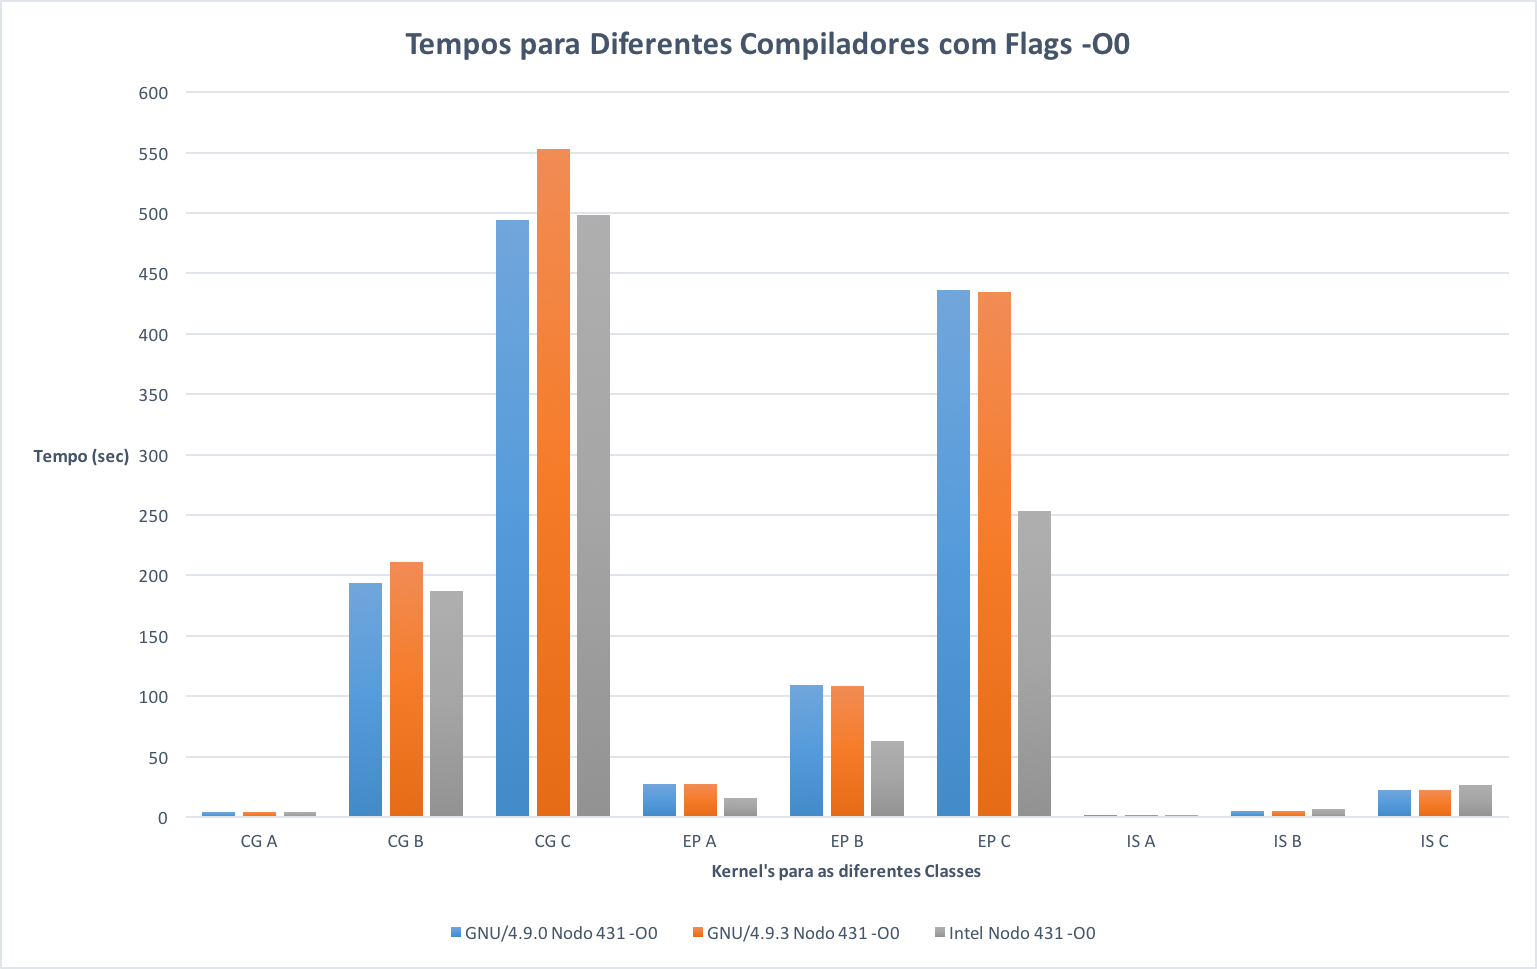
\includegraphics[scale=0.325]{SER/tempos_dif_comp_O0_nodo_431.png}
\caption{Tempos para Diferentes Compiladores com Flags -O0}
\label{fig:tempos_dif_comp_O0_431}
\end{figure}

\begin{figure}[h!]
\centering
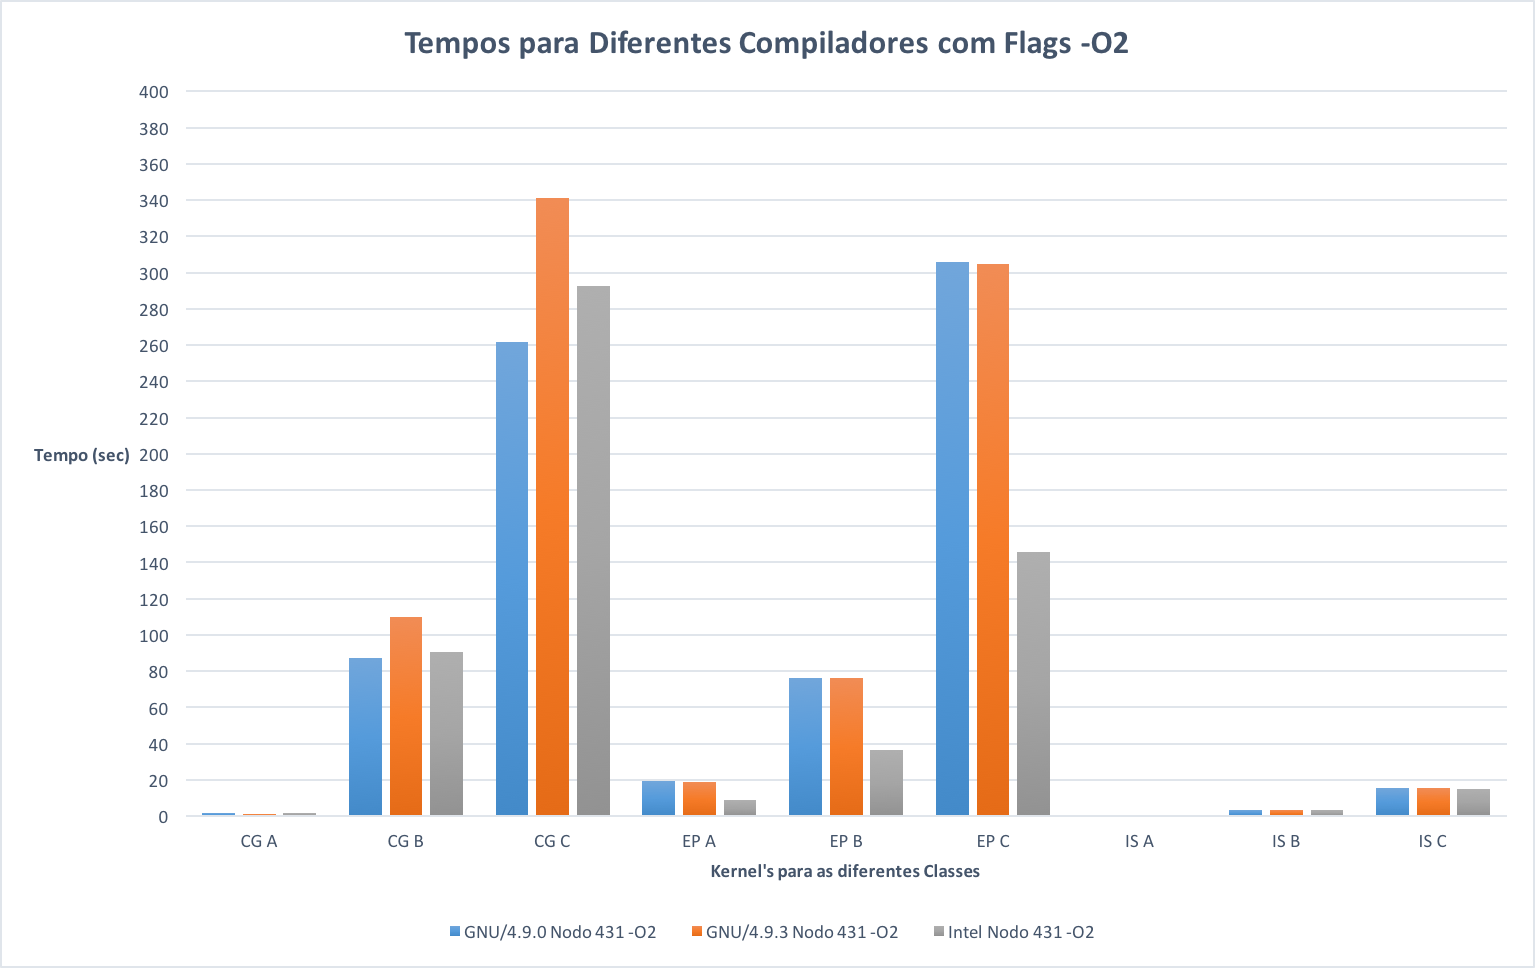
\includegraphics[scale=0.325]{SER/tempos_dif_comp_O2_nodo_431.png}
\caption{Tempos para Diferentes Compiladores com Flags -O2}
\label{fig:tempos_dif_comp_O2_431}
\end{figure}

\begin{figure}[h!]
\centering
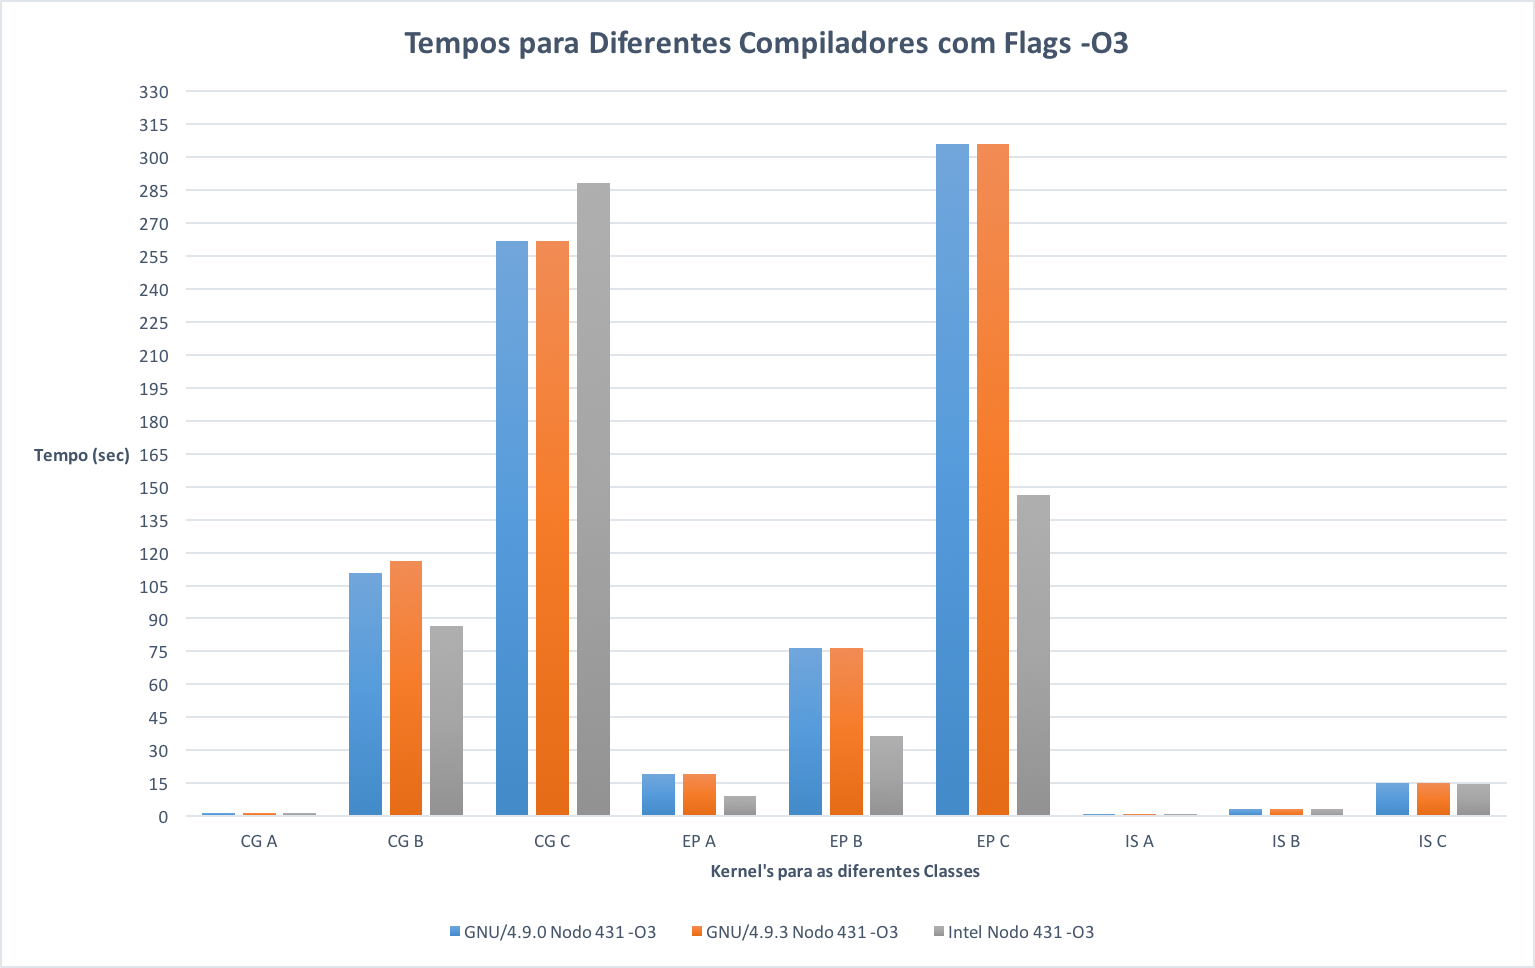
\includegraphics[scale=0.325]{SER/tempos_dif_comp_O3_nodo_431.png}
\caption{Tempos para Diferentes Compiladores com Flags -O3}
\label{fig:tempos_dif_comp_O3_431}
\end{figure}

Através da comparação dos 3 gráficos, á medida que se vai aumentando o nível de optimização, isto é, passado de -O0 para -O2 e por fim para -O3 podemos constatar que o comportamento dos compiladores é semelhante, mesmo com o aumento da Classe de dados. No caso do gráfico da figura \ref{fig:tempos_dif_comp_O3_431} para o \textit{Kernel} CG com a classe de dados B o compilador da \textit{Intel} mostra-se melhor do que os outros, neste caso o \textit{Kernel} apresenta um tempo inferior aos outros, mas se verificarmos no caso do \textit{Kernel} CG para a classe de dados C, ai o compilador da \textit{Intel} é pior que os outros dois, isto é o \textit{Kernel} compilado com o compilador da \textit{Intel} apresenta tempos de execução superiores aos outros dois. No caso do \textit{Kernel} EP (Embaraçosamente paralelo) podemos afirmar que o compilador da \textit{Intel} é melhor que os outros dois da \textit{GNU}, pois para qualquer classe de dados o \textit{Kernel} apresenta sempre tempos melhores que do que quando compilado com os compiladores da \textit{GNU}.

Nos gráficos das figuras \ref{fig:mops_dif_comp_O0_431}, \ref{fig:mops_dif_comp_O2_431} e \ref{fig:mops_dif_comp_O3_431} podemos consultar os gráficos que relacionam os MOPS para os diferentes \textit{Kernel's} para as diferentes classes de dados, para os diferentes compiladores, com a mesma flag de compilação.

Neste caso, mais uma vez, à medida que se aumenta o nível de compilação, o comportamento dos compiladores é semelhante, sendo que o \textit{Kernel} CG é o que apresenta maior numero de MOPS, no caso do gráfico da figura \ref{fig:mops_dif_comp_O3_431} este \textit{Kernel}, para a classe de dados A o compilador da \textit{Intel} é ligeiramente menos eficiente do que os outros dois da \textit{GNU}. Para a classe de dados B o compilador mais eficiente é o compilador da \textit{GNU} da versão 4.9.0, tendo este aproximadamente o mesmo valor que o \textit{Kernel} quando compilado com o compilador da \textit{intel}. Na classe de dados C para os dois compiladores da \textit{GNU} o \textit{Kernel} apresenta valores semelhantes sendo estes melhores que o \textit{Kernel} quando compilado com o compilador da \textit{Intel}. À semelhança do que acontece nos tempos, para o \textit{Kernel} EP o compilador da \textit{Intel}, mais uma vez é o mais eficiente, apresentando valores sempre superiores aos outros dois compiladores da \textit{GNU}, quer para a classe de dados A, B e C.

Os resultados para as máquinas 641 são praticamente semelhantes aos resultados das máquinas 431, isto é o comportamento á medida que se aumenta o nível de optimização é praticamente igual. Os seus gráficos podem ser consultados no anexo \ref{appendix:641_seq}

\begin{figure}[h!]
\centering
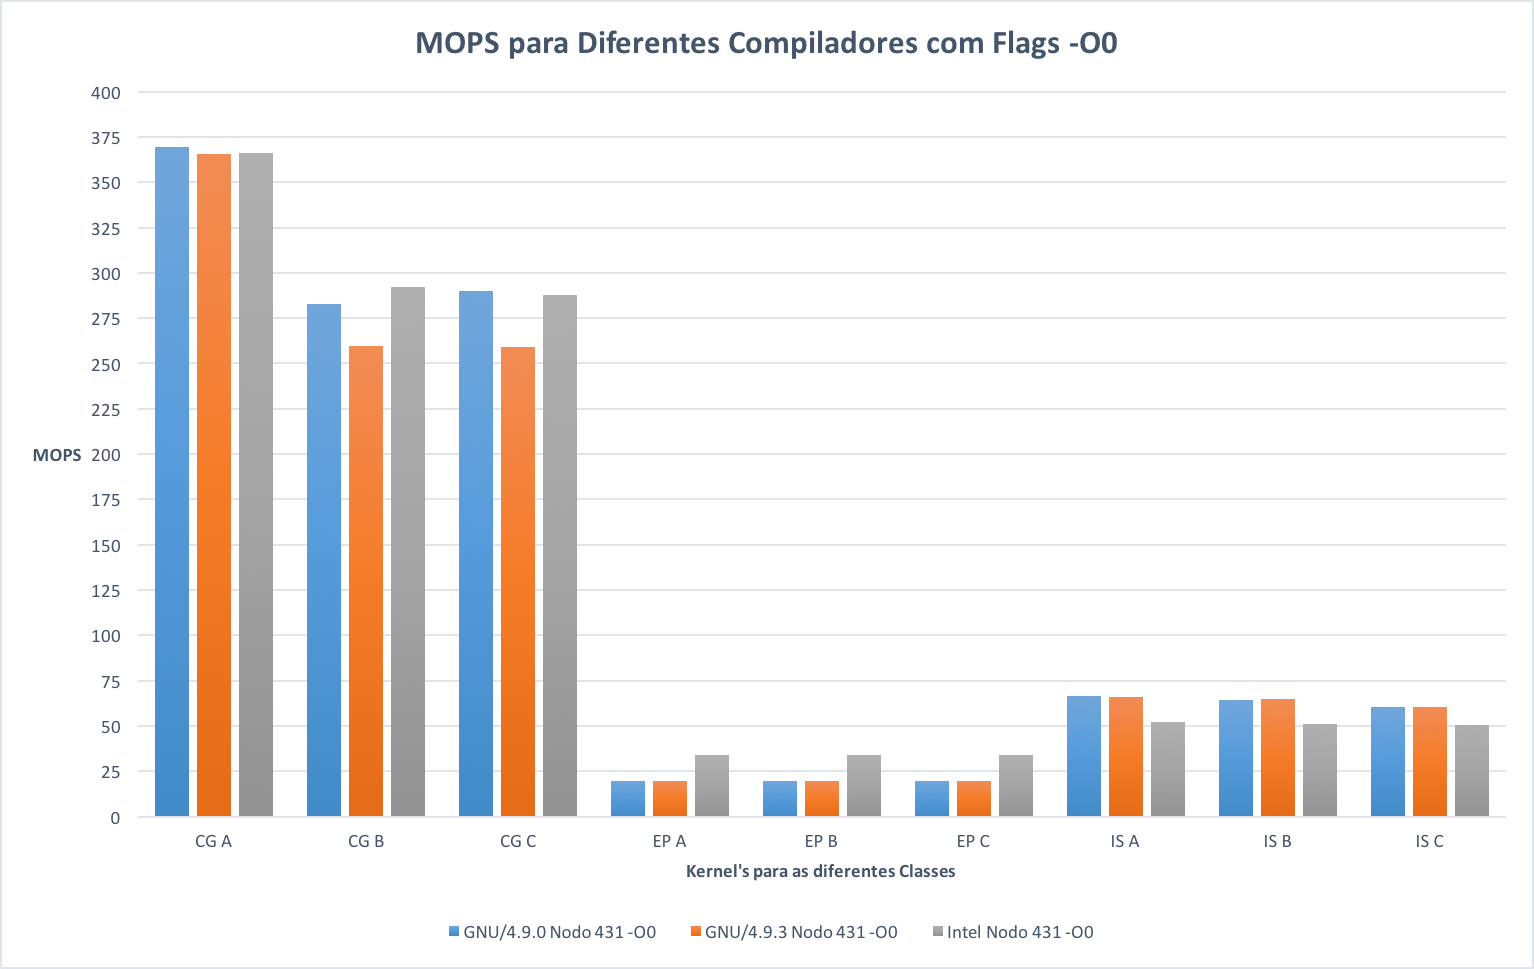
\includegraphics[scale=0.325]{SER/mops_dif_comp_O0_nodo_431.png}
\caption{MOPS para Diferentes Compiladores com Flags -O0}
\label{fig:mops_dif_comp_O0_431}
\end{figure}

\begin{figure}[h!]
\centering
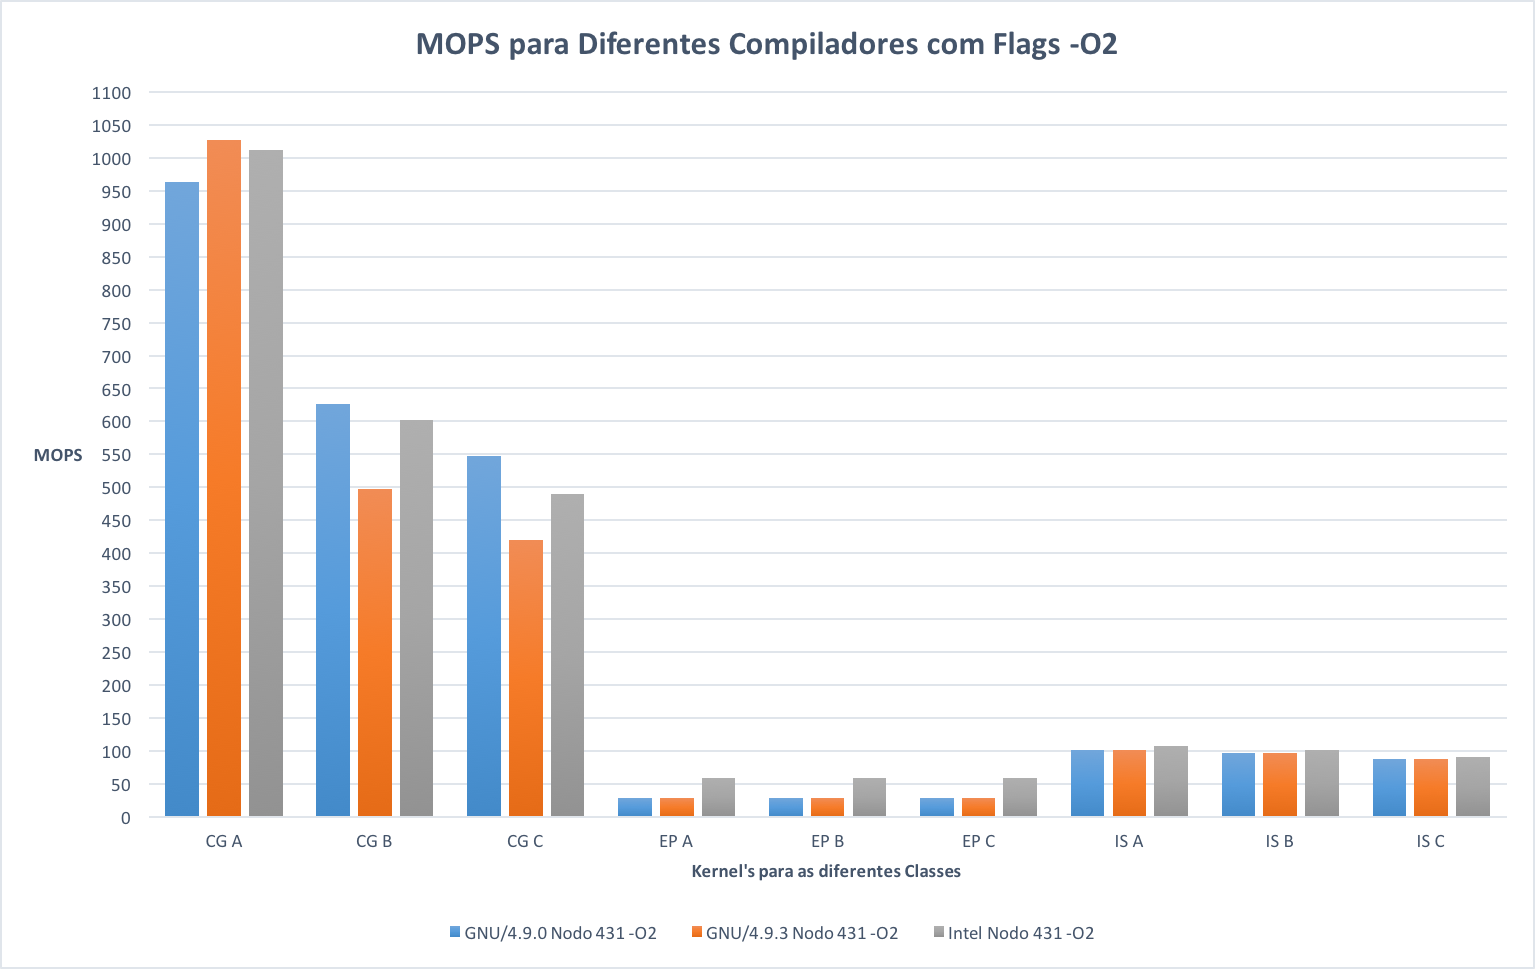
\includegraphics[scale=0.325]{SER/mops_dif_comp_O2_nodo_431.png}
\caption{MOPS para Diferentes Compiladores com Flags -O2}
\label{fig:mops_dif_comp_O2_431}
\end{figure}

\begin{figure}[h!]
\centering
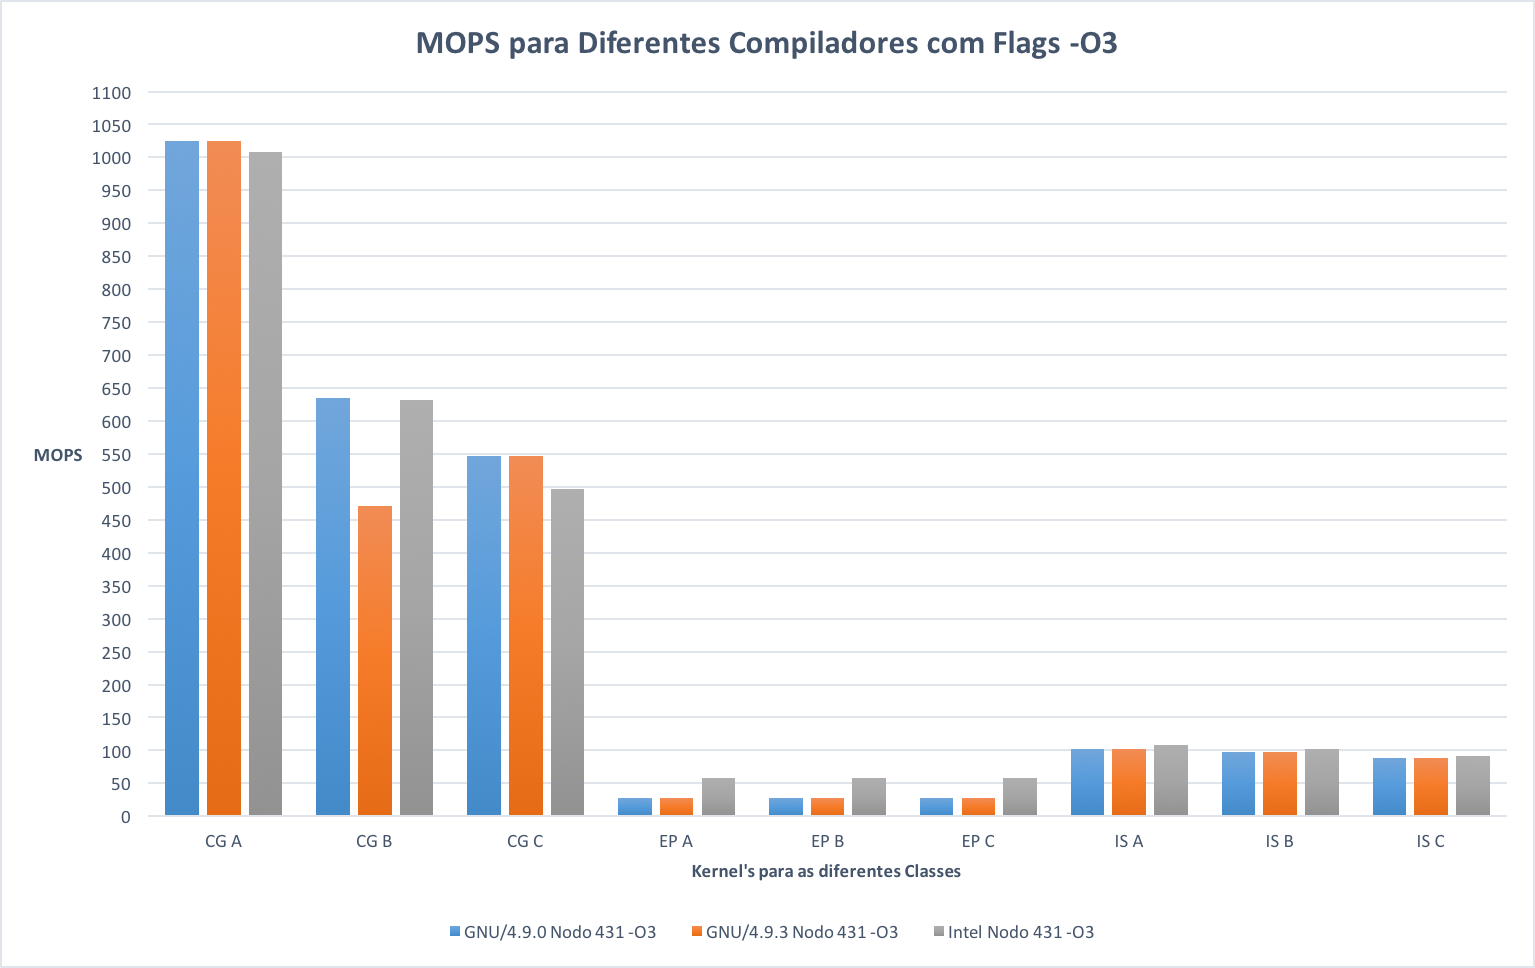
\includegraphics[scale=0.325]{SER/mops_dif_comp_O3_nodo_431.png}
\caption{MOPS para Diferentes Compiladores com Flags -O3}
\label{fig:mops_dif_comp_O3_431}
\end{figure}

\subsection{Versão OMP}
Um dos objetivos do trabalho era executar código em paralelo, neste caso com um paradigma de memória partilhada recorrendo a \textit{OpenMP}, sendo que os testes foram efetuados para 1, 2, 4, 8, 10, 12, 16, 24 e 32 \textit{Threads}. Na análise dos resultados destes testes, procurei comparar os tempos de execução, os MOPS e MOPS/Thread para os diferentes compiladores, fixando as flags de compilação para um \textit{Kernel}. De referir que devido a um grande número de gráficos que foram gerados para a versão OMP, apenas apresento uma parte dos resultados, para isso procurei apresentar os gráficos que achei que representam os melhores resultados que obtive. Como mostra a tabela \ref{t:testes_omp_431} e a tabela \ref{t:testes_omp_641} para esta versão apenas efetuei testes com as flags de compilação -O2 e -O3. De notar que os gráficos apresentados dizem respeito aos testes efetuados nas máquinas 431.

\begin{figure}[h!]
\centering
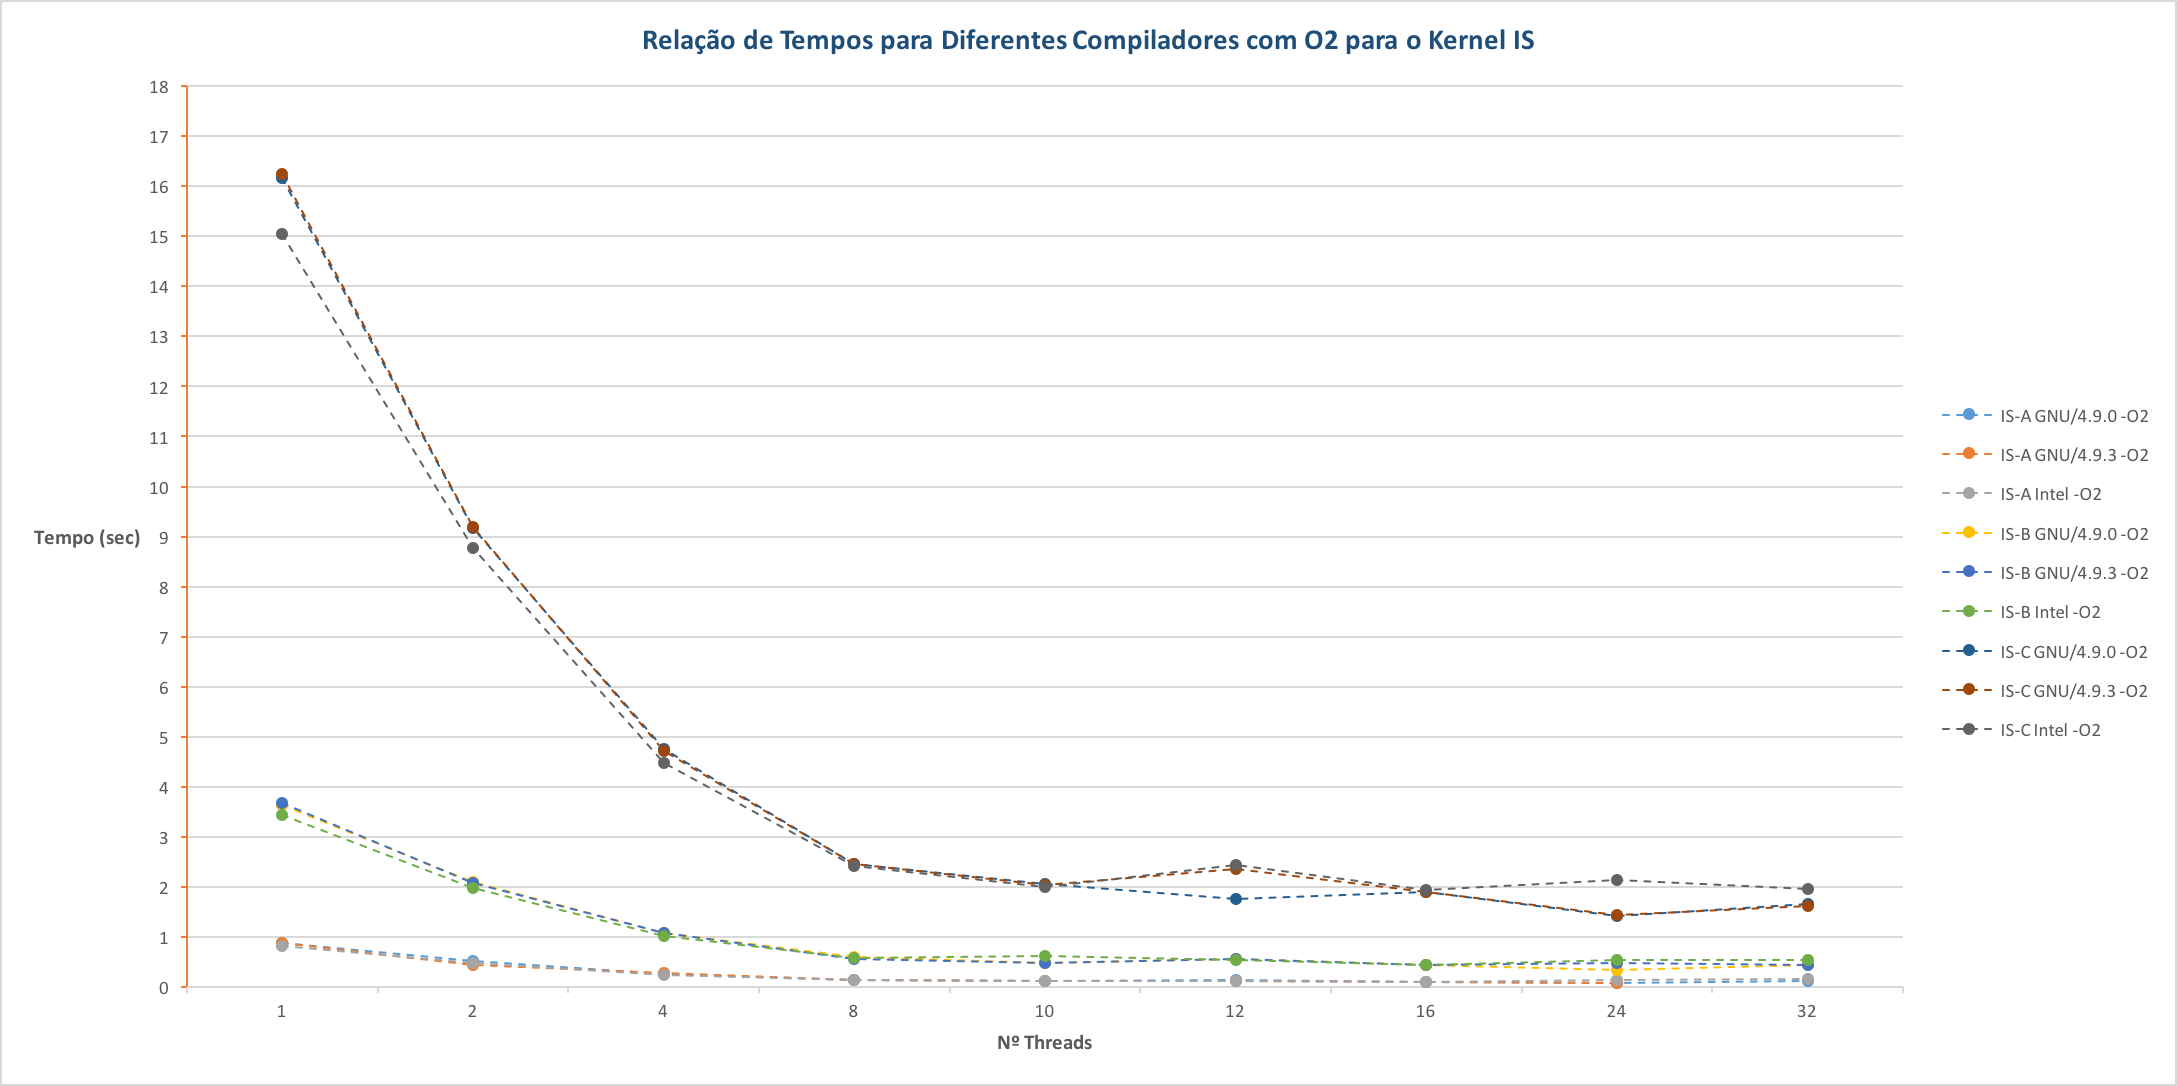
\includegraphics[scale=0.25]{OMP/tempos_dif_comp-O2_IS_nodo-431.png}
\caption{Tempos para Diferentes Compiladores com Flags -O2 para o \textit{Kernel} IS}
\label{fig:tempos_dif_comp_omp_O2_IS_431}
\end{figure}

\begin{figure}[h!]
\centering
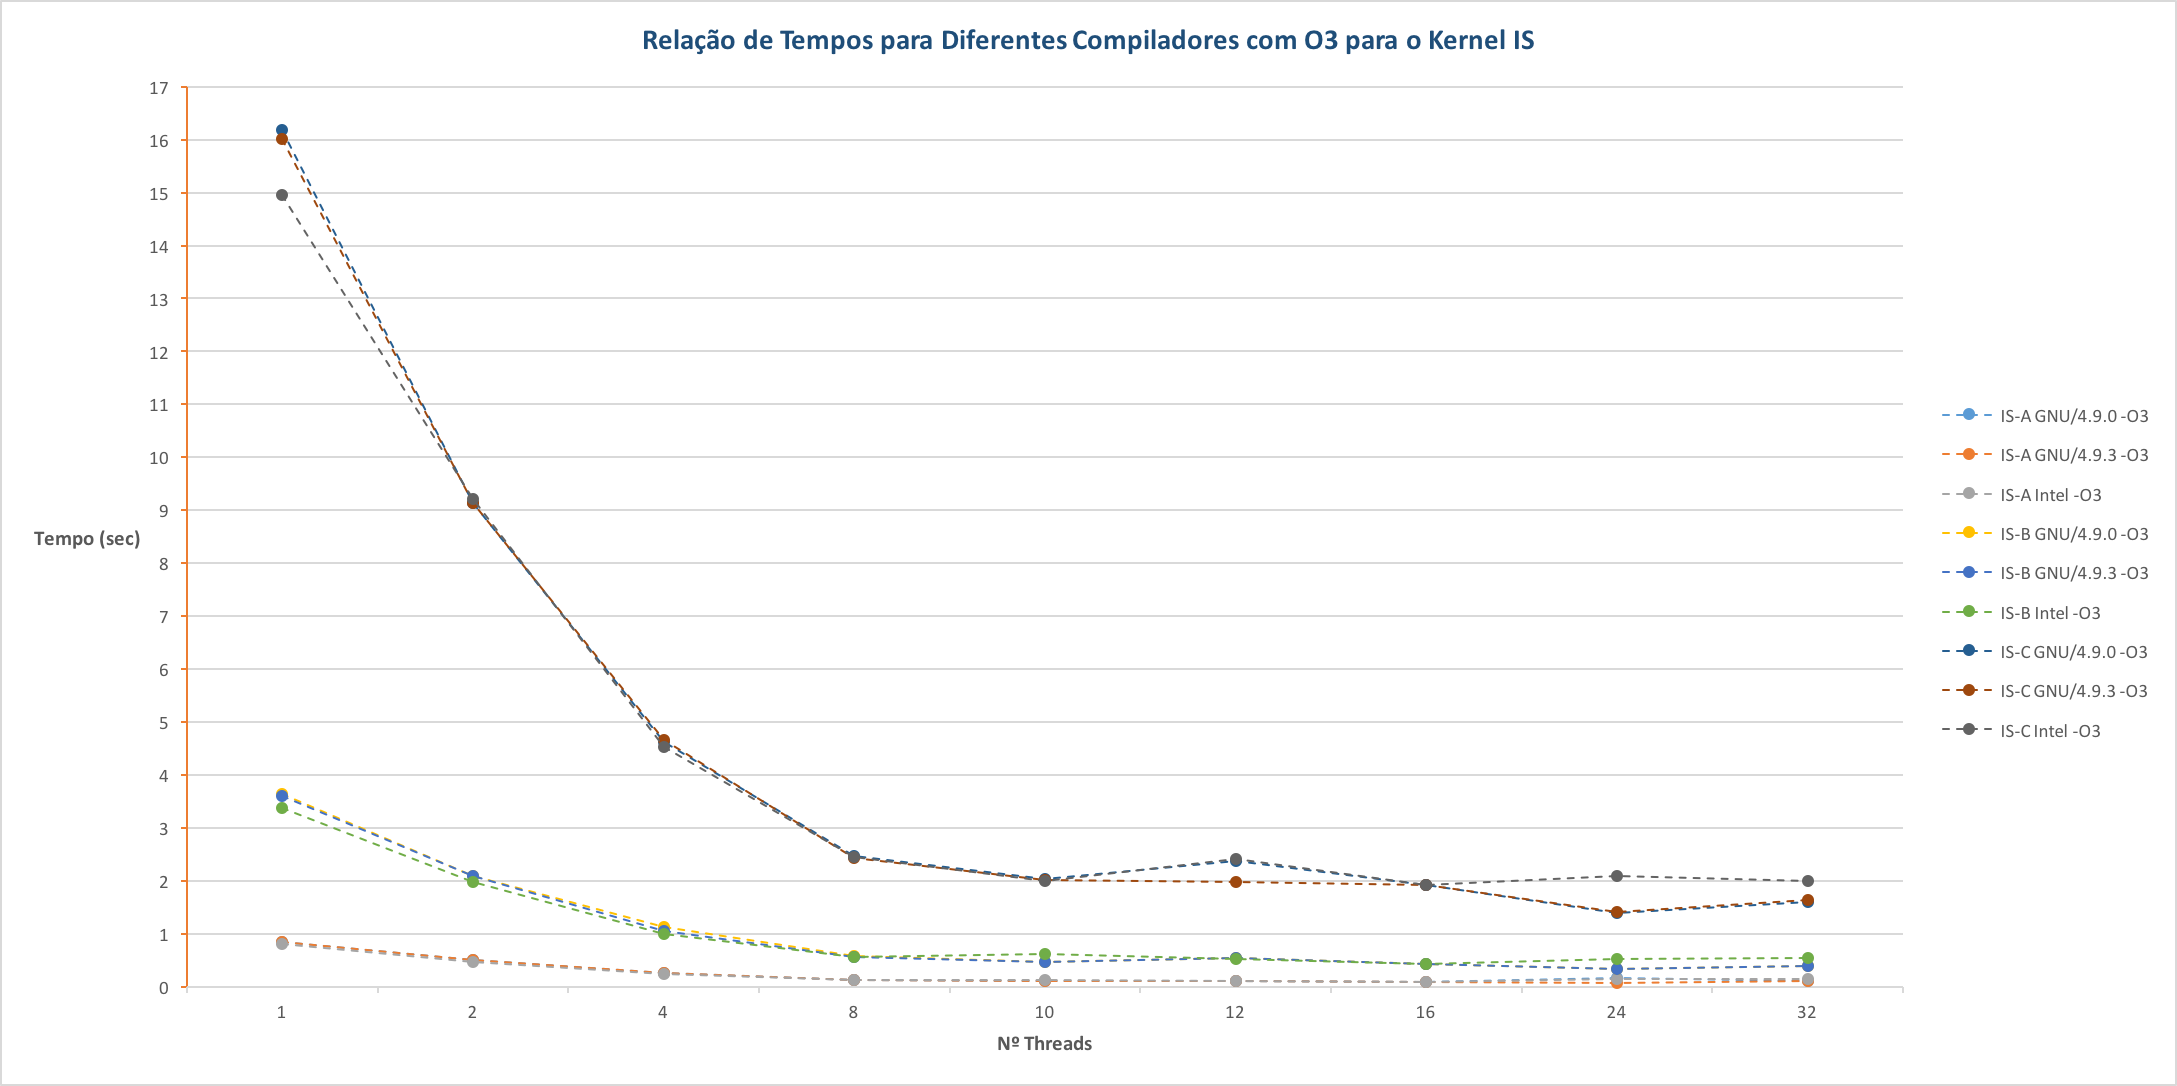
\includegraphics[scale=0.25]{OMP/tempos_dif_comp-O3_IS_nodo-431.png}
\caption{Tempos para Diferentes Compiladores com Flags -O3 para o \textit{Kernel} IS}
\label{fig:tempos_dif_comp_omp_O3_IS_431}
\end{figure}

Escolhi os gráficos do \textit{Kernel} IS, pois foi o \textit{Kernel} para o qual obtive um tempo de execução inferior. Como podemos verificar pela a análise do gráfico da figura \ref{fig:tempos_dif_comp_omp_O2_IS_431} e do gráfico da figura \ref{fig:tempos_dif_comp_omp_O3_IS_431} há pouca variação dos tempos quer na versão compilada com a flag -O2, quer com a flag -O3, tanto um gráfico como o outro são praticamente iguais. 

No gráfico da figura \ref{fig:tempos_dif_comp_omp_O2_IS_431} com flag -O2 o \textit{Kernel} IS atinge o seu menor tempo para o compilador gnu/4.9.0 com 24 \textit{Threads} tanto para a classe de dados A, B e C com tempos de 0.08 segundos, 0.33 segundos e 1.41 segundos respetivamente. Para o compilador gnu/4.9.3 com flag -O2 o \textit{Kernel} atinge o menor tempo para a classe A com 24 \textit{Threads} bem como para a classe C com tempos de 0.08 segundos e 1.44 segundos respetivamente, para a classe B o \textit{Kernel} atinge o menor tempo tanto com 16 \textit{Threads} como com 24 \textit{Threads} com valor de 0.44 segundos. Quanto ao compilador da \textit{Intel}, com flag -O2 o \textit{Kernel} atinge o seu menor tempo com 16 \textit{Threads}, quer para a classe A, B e C com tempos de 0.1 segundos, 0.43 segundos e 1.93 segundos respetivamente. Podemos assim concluir que para este \textit{Kernel} com flag -O2, independentemente da classe de dados o compilador da \textit{Intel} é o mais eficiente.

No gráfico da figura \ref{fig:tempos_dif_comp_omp_O3_IS_431}, com flag -O3, para o compilador gnu/4.9.0 o \textit{Kernel} IS atinge o seu menor tempo para a classe A com 16 \textit{Threads}, tendo um valor de 0.1 segundos e para as classes de dados B e C atinge o menor tempo com 24 \textit{Threads}, com tempos de 0.34 segundos e 1.4 segundos respetivamente. Para o compilador da gnu/4.9.3, com flag -O3 o \textit{Kernel} atinge o seu menor tempo com 24 \textit{Threads}, quer para a classe A, B e C, com tempos de 0.08 segundos, 0.35 segundos e 1.41 segundos respetivamente. No que toca ao compilador da \textit{Intel} com flag -O3 o \textit{Kernel} atinge o seu menor tempo com 16 \textit{Threads}, com tempos de 0.1 segundos, 0.43 segundos e 1.92 segundos respetivamente. À semelhança do que acontece com o caso anterior, isto é, quando o \textit{Kernel} é compilado com -O2, aqui o compilador da \textit{Intel} também mostra ser o mais eficiente, com flag -O3.

\begin{figure}[h!]
\centering
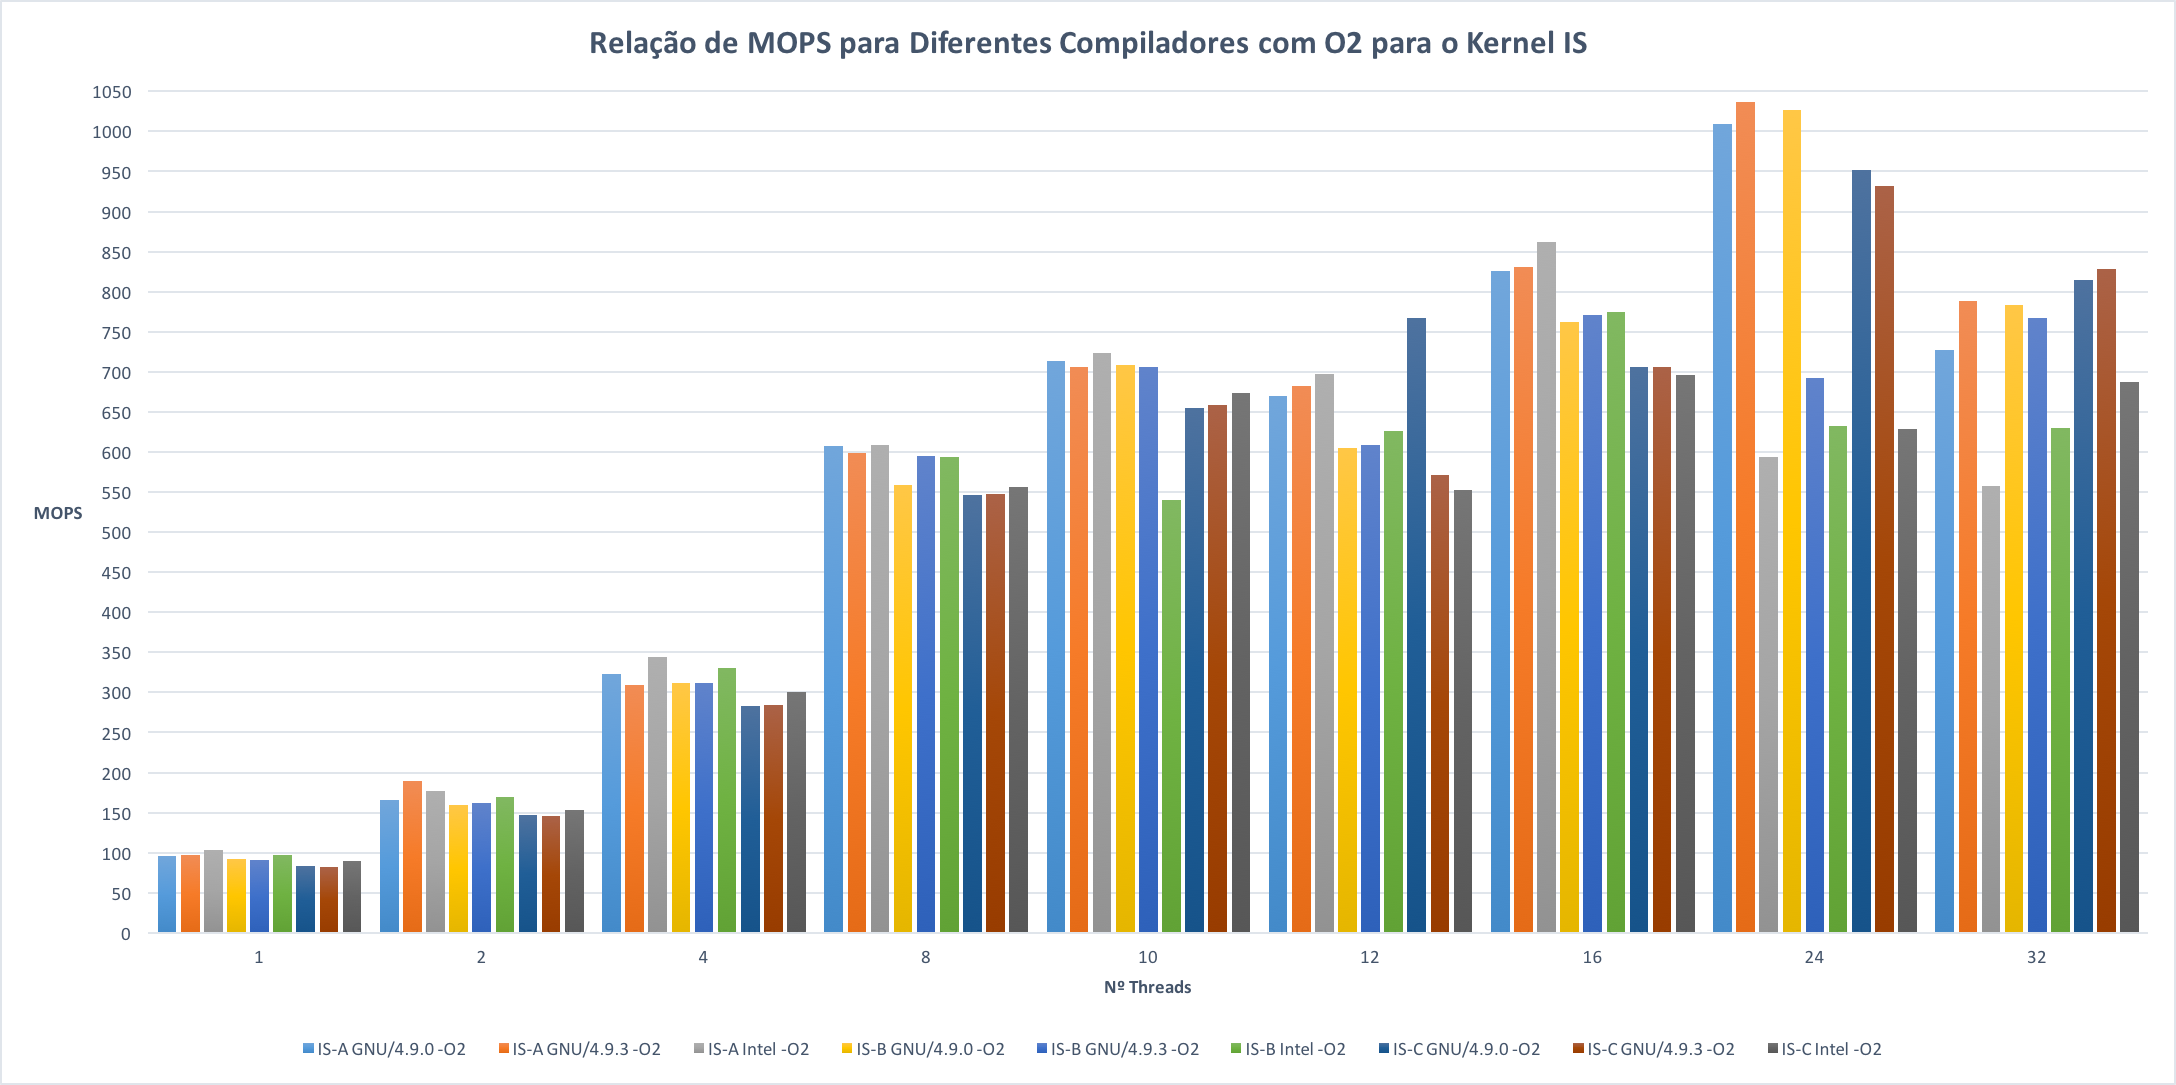
\includegraphics[scale=0.225]{OMP/mops_dif_comp-O2_IS_nodo-431.png}
\caption{MOPS para Diferentes Compiladores com Flags -O2 para o \textit{Kernel} IS}
\label{fig:mops_dif_comp_omp_O2_IS_431}
\end{figure}

\begin{figure}[h!]
\centering
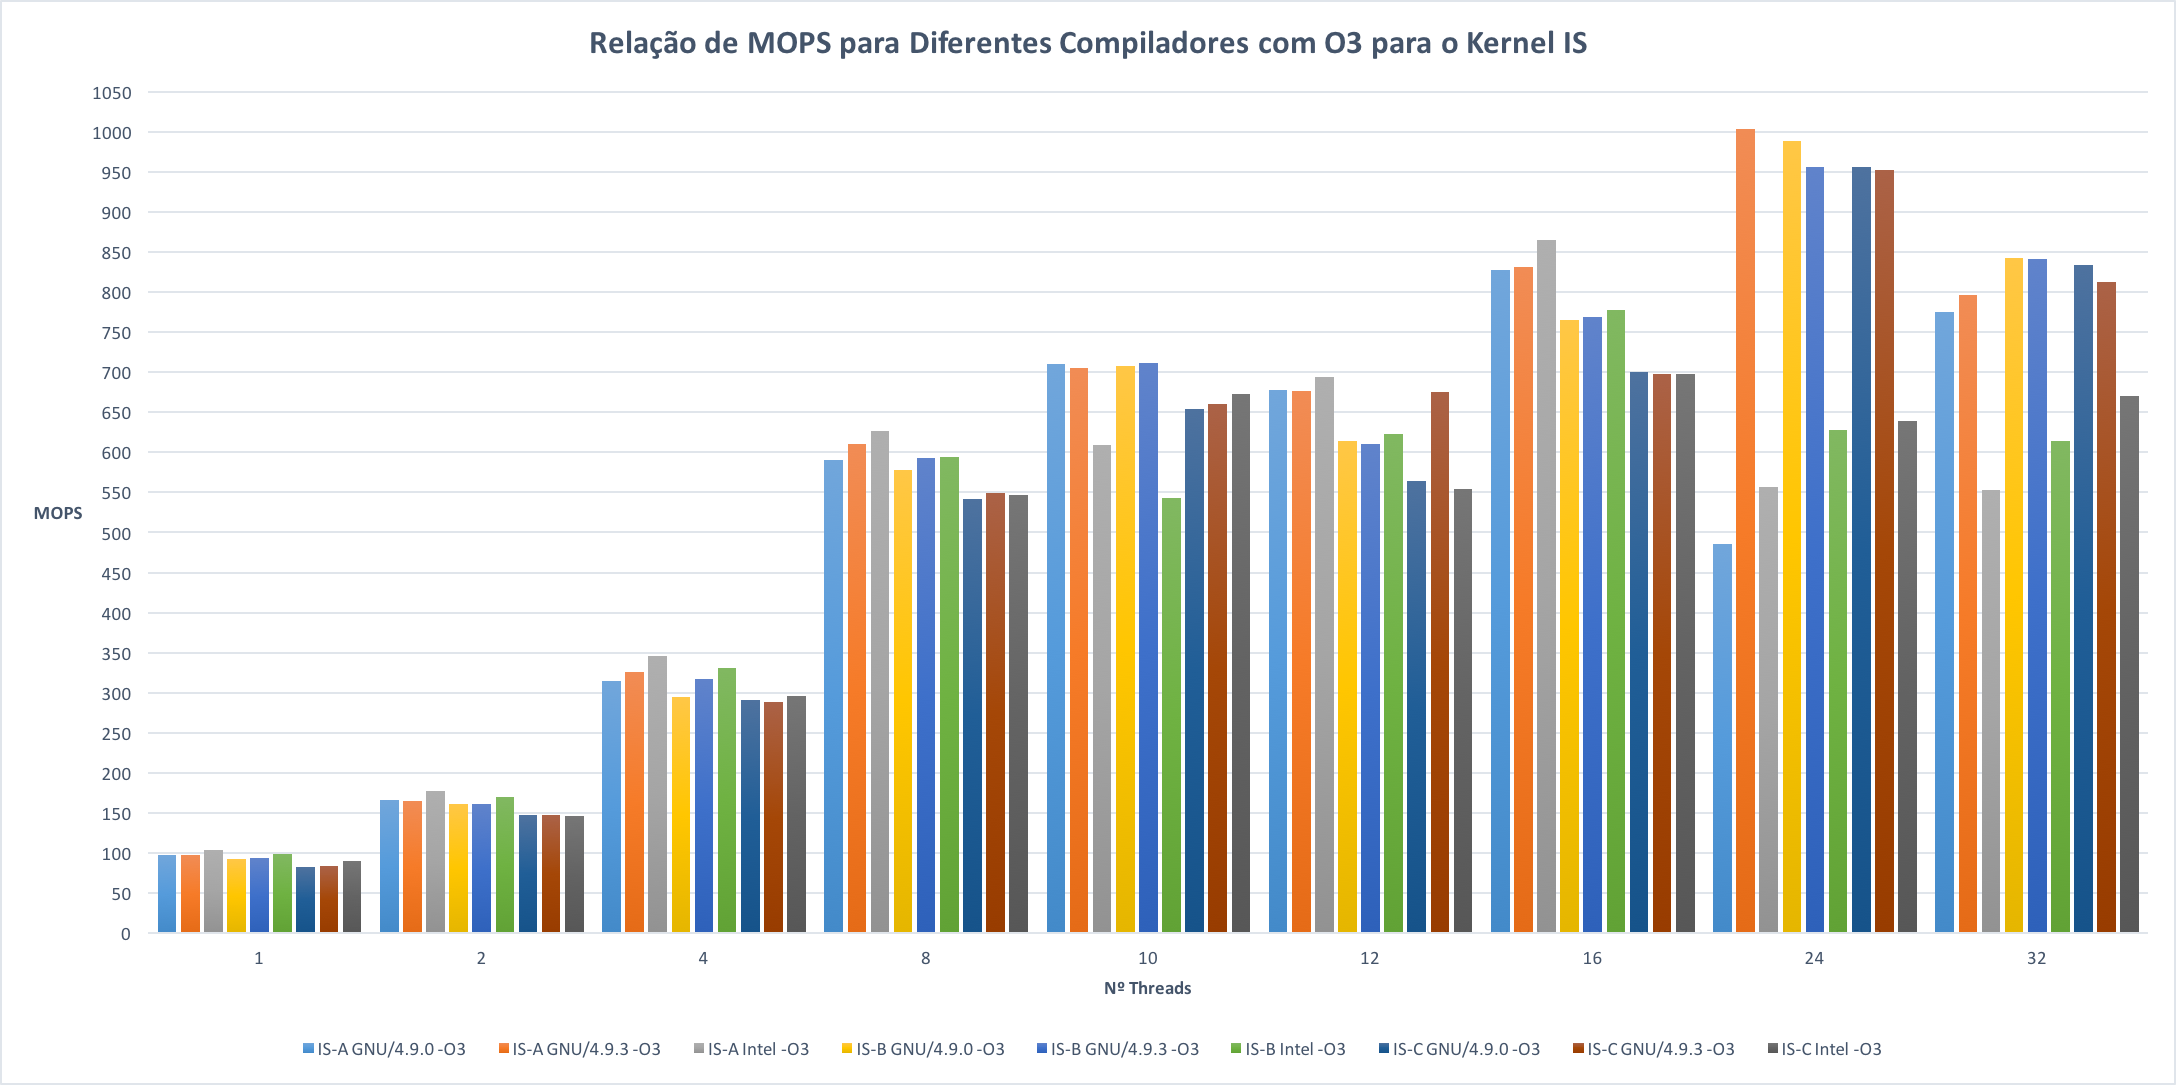
\includegraphics[scale=0.225]{OMP/mops_dif_comp-O3_IS_nodo-431.png}
\caption{MOPS para Diferentes Compiladores com Flags -O3 para o \textit{Kernel} IS}
\label{fig:mops_dif_comp_omp_O3_IS_431}
\end{figure}

Quanto aos MOPS como podemos verificar nos gráficos da figura \ref{fig:mops_dif_comp_omp_O2_IS_431} e no gráfico da figura \ref{fig:mops_dif_comp_omp_O3_IS_431}, estes tendem a aumentar até às 24 \textit{Threads}, tanto com flag -O2 como com flag -O3. Em oposição os MOPS/\textit{Thread} tendem a diminuir com o aumento do número de \textit{Threads} tanto com flag -O2 como com flag -O3, como mostra o gráfico da figura \ref{fig:mops-thread_dif_comp_omp_O2_IS_431} e o gráfico da figura \ref{fig:mops-thread_dif_comp_omp_O3_IS_431}, o que já era de esperar.

\begin{figure}[h!]
\centering
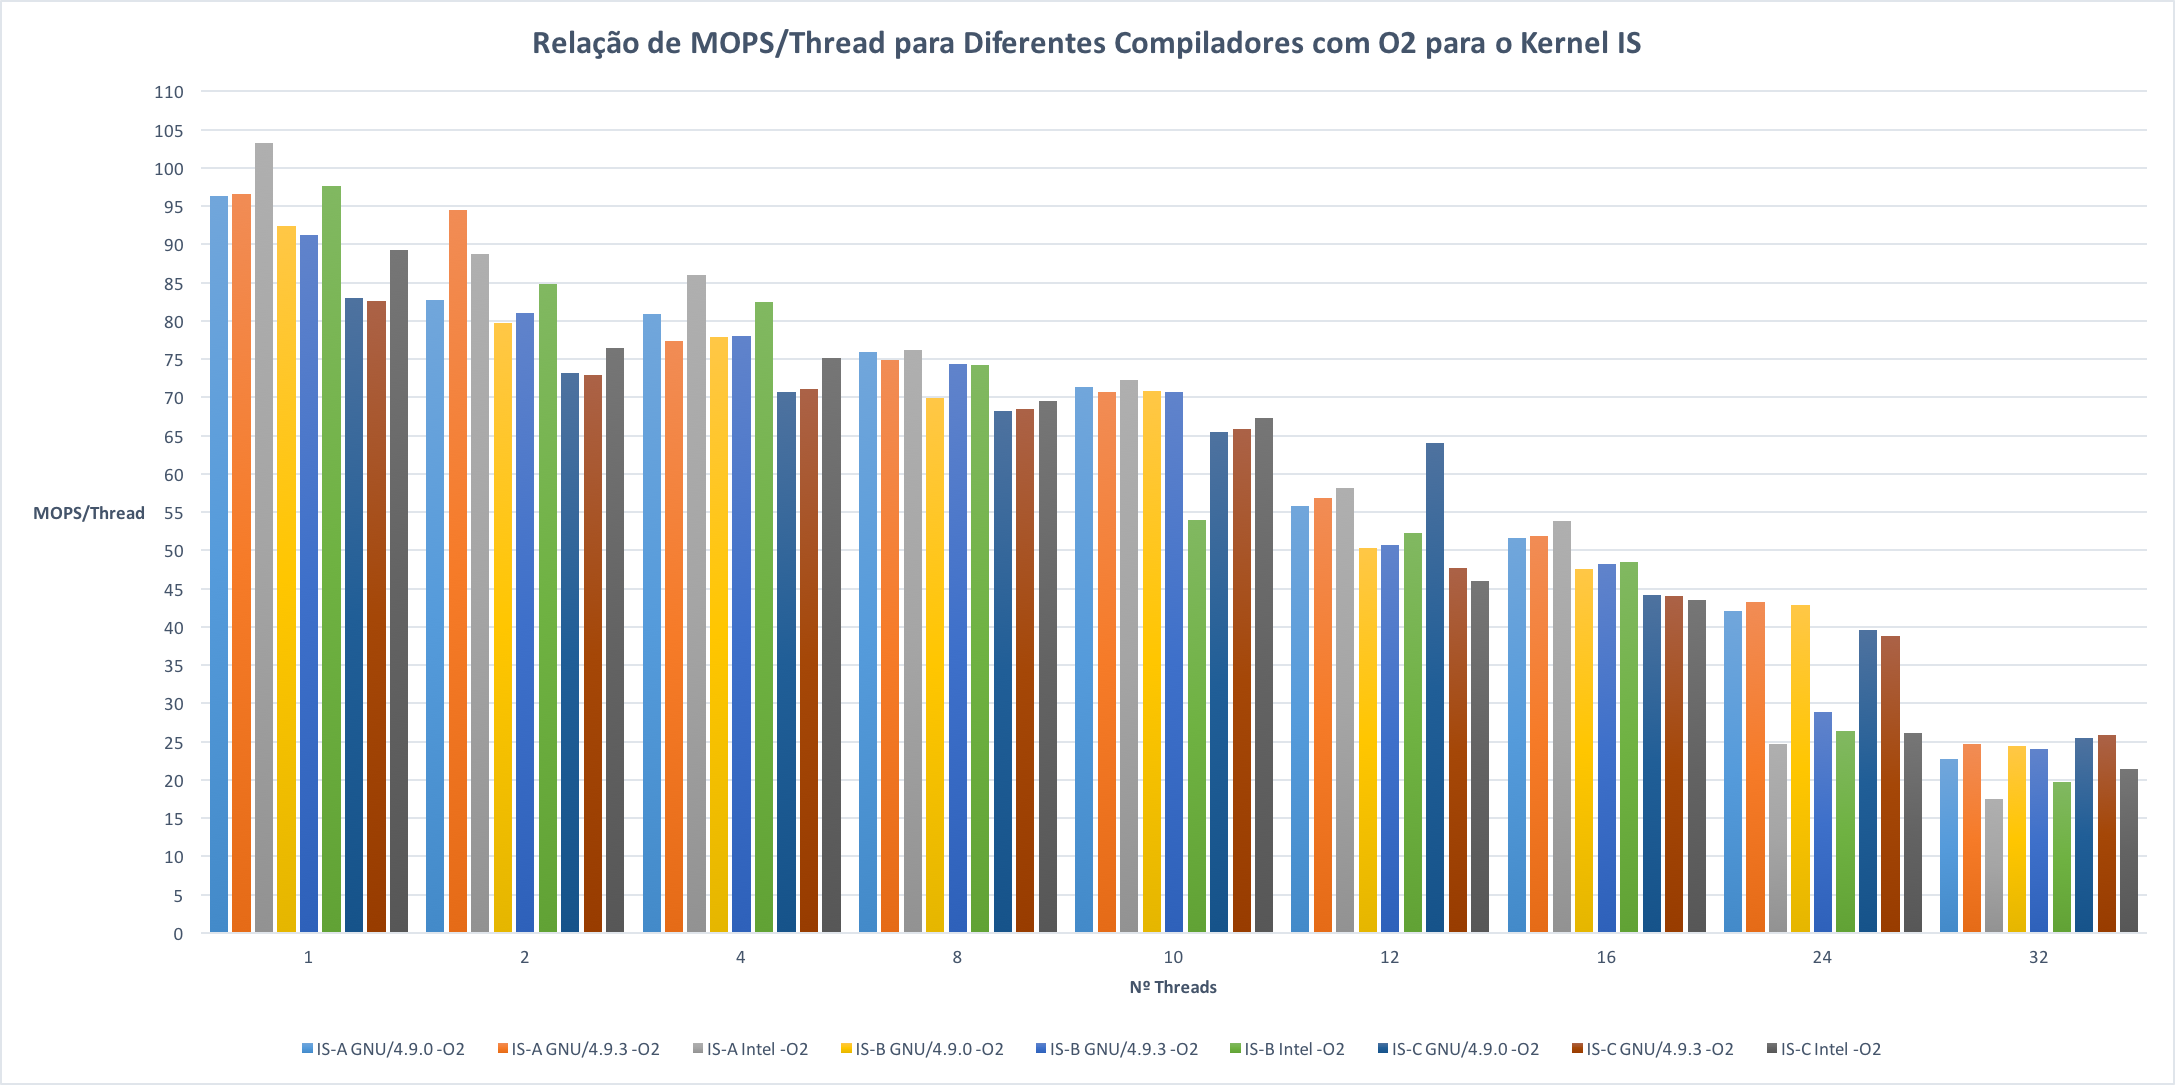
\includegraphics[scale=0.225]{OMP/mops-thread_dif_comp-O2_IS_nodo-431.png}
\caption{MOPS/\textit{Thread} para Diferentes Compiladores com Flags -O2 para o \textit{Kernel} IS}
\label{fig:mops-thread_dif_comp_omp_O2_IS_431}
\end{figure}

\begin{figure}[h!]
\centering
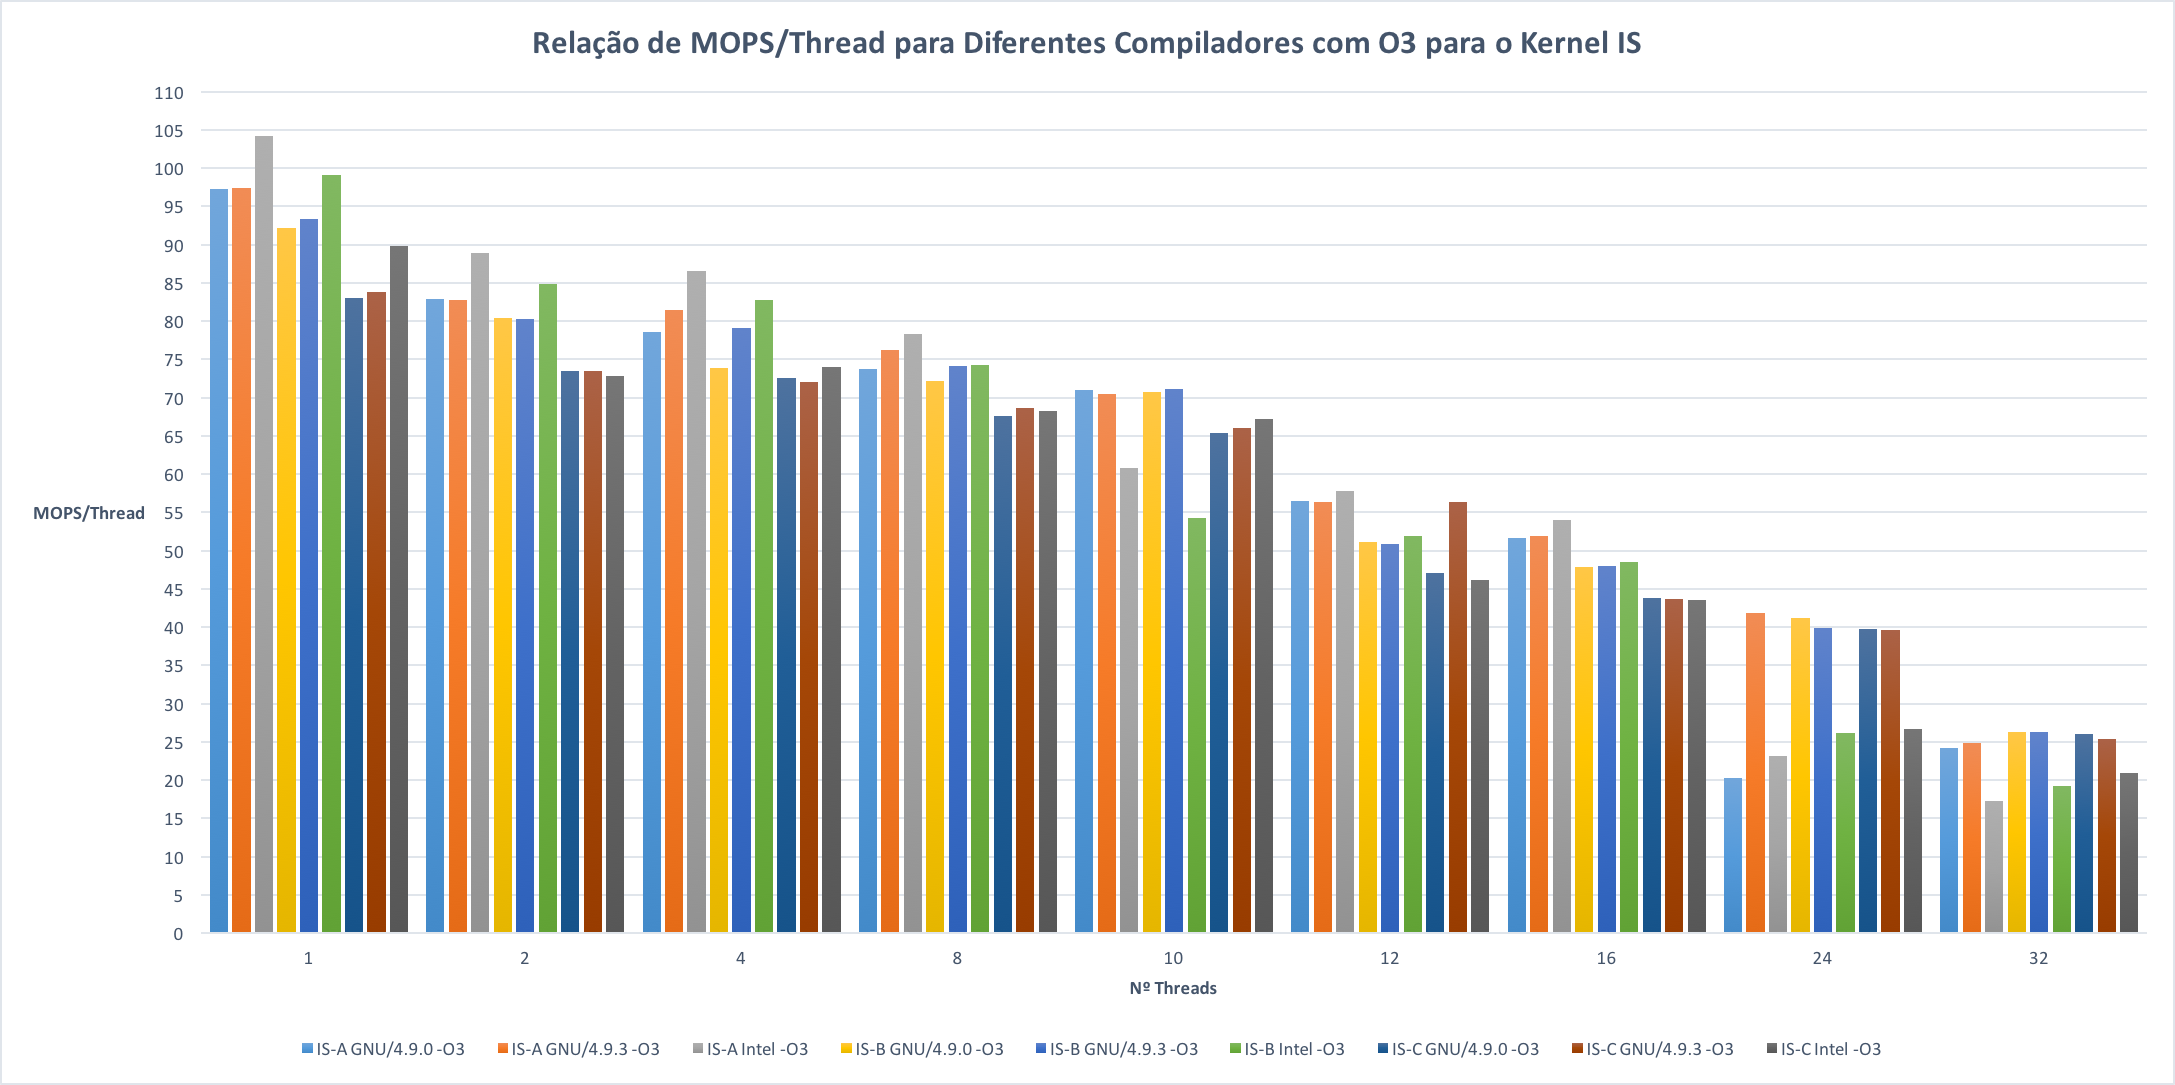
\includegraphics[scale=0.225]{OMP/mops-thread_dif_comp-O3_IS_nodo-431.png}
\caption{MOPS/\textit{Thread} para Diferentes Compiladores com Flags -O3 para o \textit{Kernel} IS}
\label{fig:mops-thread_dif_comp_omp_O3_IS_431}
\end{figure}

Os gráficos para o \textit{Kernel} IS nas máquinas 641 podem ser consultados no anexo \ref{appendix:641_omp}.

\subsection{Versão MPI}
Para alem da versão paralela OMP, era também objetivo deste trabalho efetuar testes com um paradigma de memória distribuída, neste caso MPI. Nesta versão efetuei testes para ethernet quer com compiladores da intel, quer com compiladores da gnu, testei com 8, 16 e 32 processos para cada classe de dados. De notar que os dados apresentados, dizem respeito a testes efetuados nas máquinas 641, apenas com \textit{Ethernet} uma vez que não consegui obter dados para a execução com \textit{Myrinet}.

\begin{figure}[h!]
\centering
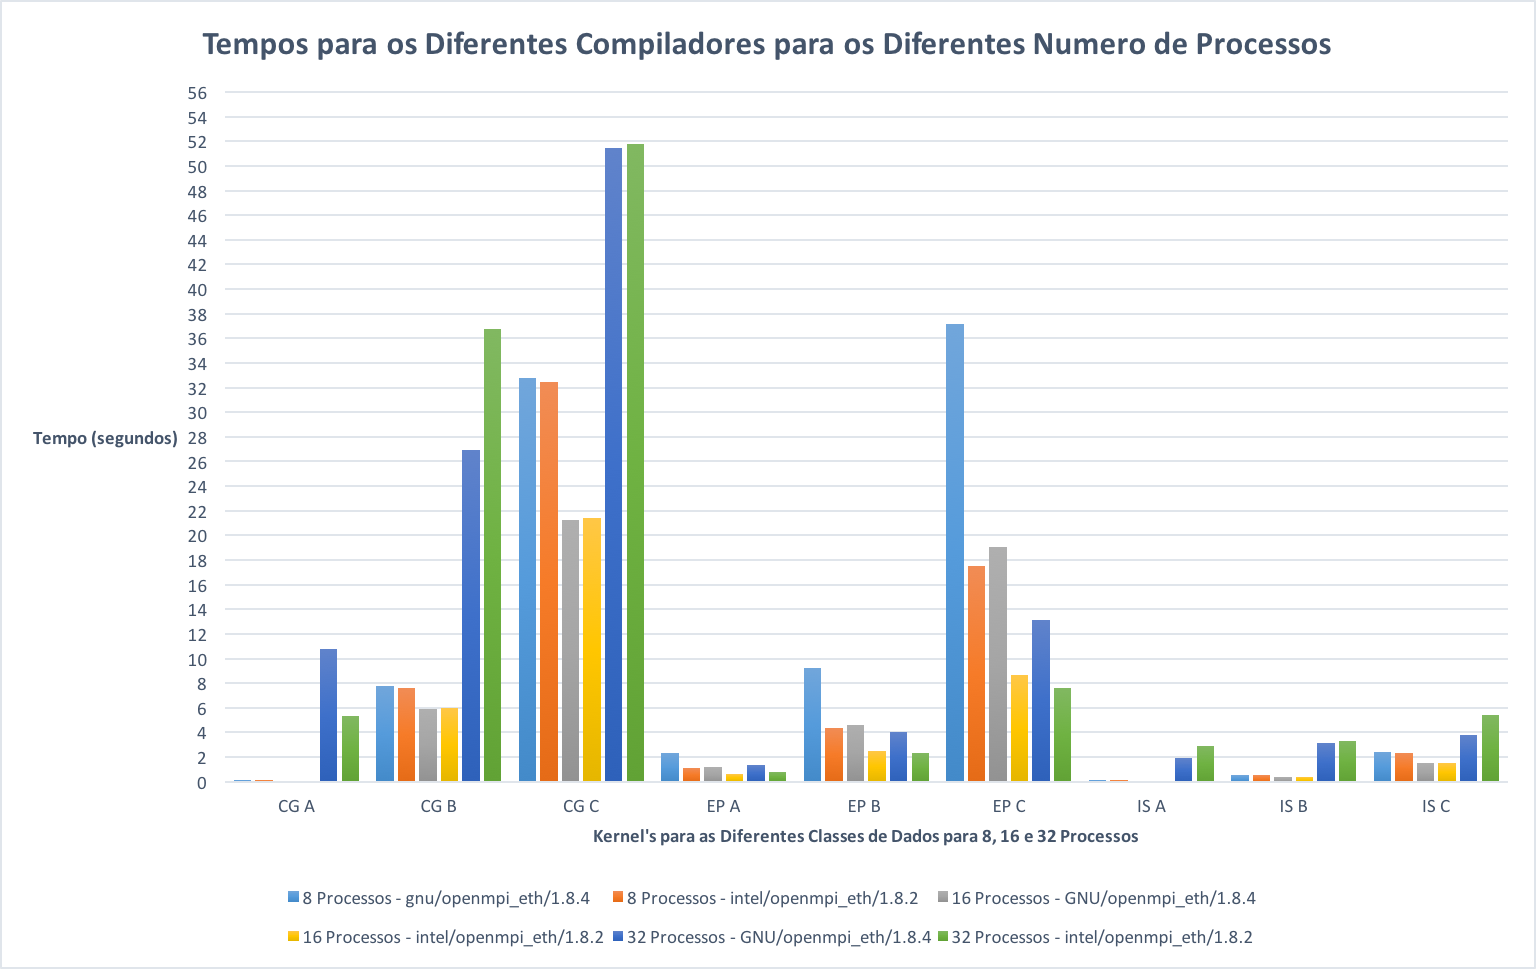
\includegraphics[scale=0.325]{MPI/tempos_dif_compiladores_dif_num_proc.png}
\caption{Tempos para os Diferentes Compiladores para os Diferentes Números de processos}
\label{fig:tempo_mpi_eth}
\end{figure}

No gráfico da figura \ref{fig:tempo_mpi_eth} podemos consultar os tempos de cada \textit{Kernel} para as diferentes classes da dados numa execução com 8 processos, 16 processos e 32 processos. Como podemos analisar o \textit{Kernel} CG atinge o seu menor tempo, independentemente da classe de dados, com 8 processos, quer para o compilador da \textit{GNU}, quer com o compilador da \textit{Intel}. 

No que diz respeito ao \textit{Kernel} EP (Embaraçosamente Paralelo), este atinge o seu menor tempo com 32 processos para as classes de dados B e C com o compilador da \textit{Intel} e para a classe A atinge o seu menor tempo com 16 processos mas também com o compilador da \textit{Intel}. Por isto para este Kernel podemos concluir que o compilador da \textit{Intel} é o mais eficiente.

Por fim o \textit{Kernel} IS atinge o seu melhor tempo com 16 processos, qualquer que seja a sua classe de dados, sendo que os tempos de execução entre dois os compiladores, são muito próximos um do outro.

\begin{figure}[h!]
\centering
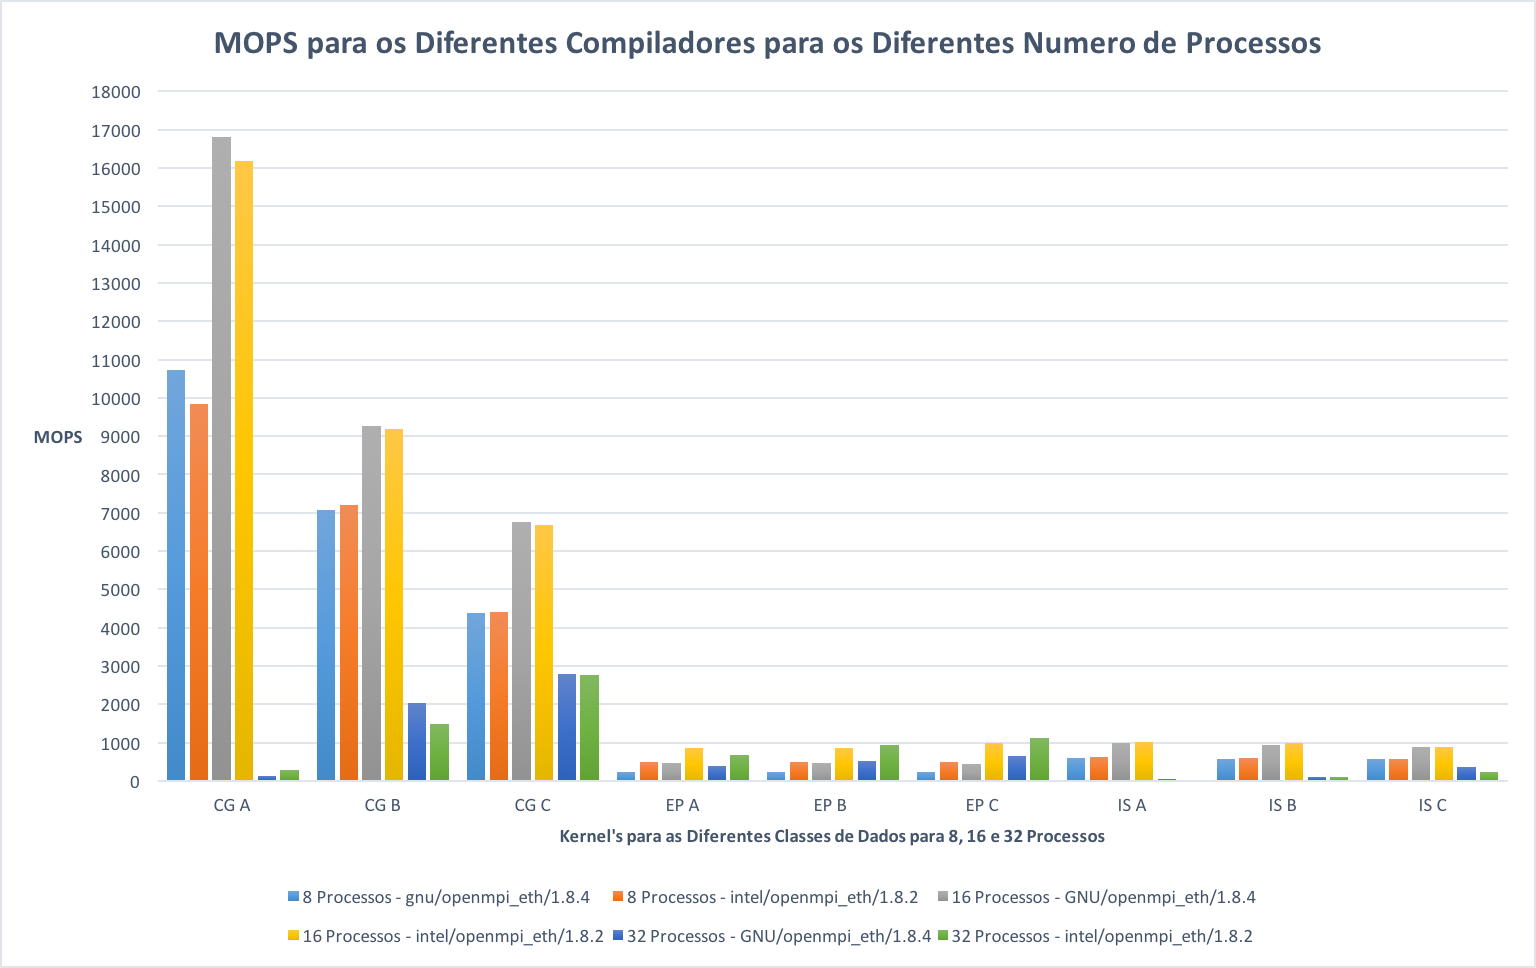
\includegraphics[scale=0.325]{MPI/mops_dif_compiladores_dif_num_proc.png}
\caption{MOPS para os Diferentes Compiladores para os Diferentes Números de processos}
\label{fig:mops_mpi_eth}
\end{figure}

Quanto aos MOPS, podemos analisar o gráfico da figura \ref{fig:mops_mpi_eth}, como podemos ver os MOPS para o \textit{Kernel} CG tendem a diminuir com 8 processos e com 16 processos, com o aumento da classe de dados sendo que com 32 processos, estes tendem a aumentar, ao aumentar a classe de dados. Pela a análise do gráfico podemos concluir que para o \textit{Kernel} CG é mais eficiente executá-lo com 16 processos, uma vez que para as diferentes classes de dados, é com 16 processos que os MOPS são maiores.

No \textit{Kernel} EP os MOPS apresentam aproximadamente os mesmos valores, quer para 8 e 16 processos, como pode ser comprovado pelo gráfico da figura \ref{fig:mops_mpi_eth}, contudo, para 32 processos os MOPS aumentão ligeiramente com o aumento das classes de dados. Neste \textit{Kernel} para as classes de dados B e C, o mais eficiente é executar o \textit{Kernel} com 32 processos com o compilador da \textit{Intel}, sendo que para a classe de dados A, o mais eficiente é excutar o \textit{Kernel} com 16 processos, com o compilador da \textit{GNU}.

Por fim no \textit{Kernel} IS os MOPS, mais uma vez tendem a ter aproximadamente os mesmos valores, havendo pouca variação, à medida que se aumenta a classe de dados, contudo é com 16 processos, que a execução deste \textit{Kernel} mostra ser mais eficiente, tanto com o compilador da \textit{GNU} como com o compilador da \textit{Intel}.

\begin{figure}[h!]
\centering
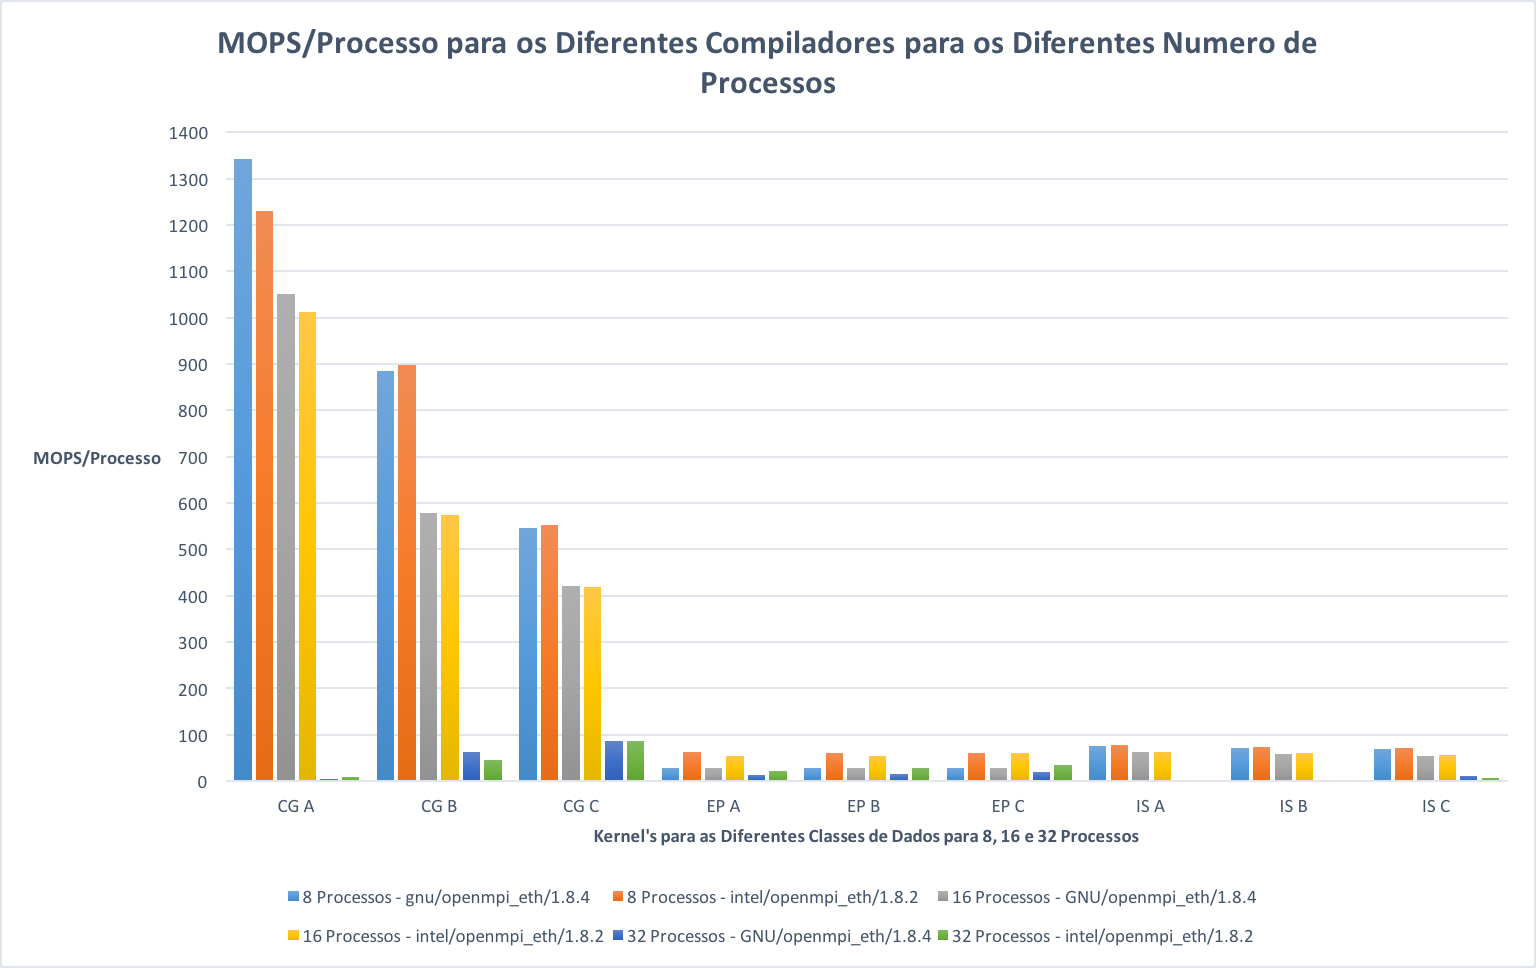
\includegraphics[scale=0.325]{MPI/mops-process_dif_compiladores_dif_num_proc.png}
\caption{MOPS para os Diferentes Compiladores para os Diferentes Números de processos}
\label{fig:mops-process_mpi_eth}
\end{figure}

O gráfico da figura \ref{fig:mops-process_mpi_eth} mostra a relação entre os diferentes \textit{Kernel's} para as diferentes classes de dados, para 8, 16 e 32 processos. Pela a análise do gráfico, podemos verificar que para o \textit{Kernel CG} á medida que se aumenta a classe de dados, de A até C os MOPS por processo diminuem, para 8 e 16 processos, sendo que para 32 processos, estes aumentam para os dois compiladores, o que já era de esperar uma vez que o comportamento dos MOPS é o mesmo.

No \textit{Kernel} EP o comportamento dos MOPS por processo é semelhante ao comportamento dos MOPS, isto é, tendem a ter os mesmo valores (aproximadamente), à medida que se aumenta a classe de dados. Para o \textit{Kernel} IS, os MOPS por processo tendem a ter os mesmos valores, à semelhança do que acontece com no gráfico da figura \ref{fig:mops_mpi_eth}.

\section{Ganhos}\label{sec:ganhos}

No que toca aos ganhos, decidi filtrar um bocado os dados uma vez que, caso não o fizesse o relatório iria ficar muito extenso. Com isto, decidi escolher o \textit{Kernel} IS com as classes de dados A, B e C, compilado com o compilador da \textit{Intel} com flag -O3.

\subsection{Sequencial vs OMP}

\begin{figure}[h!]
\centering
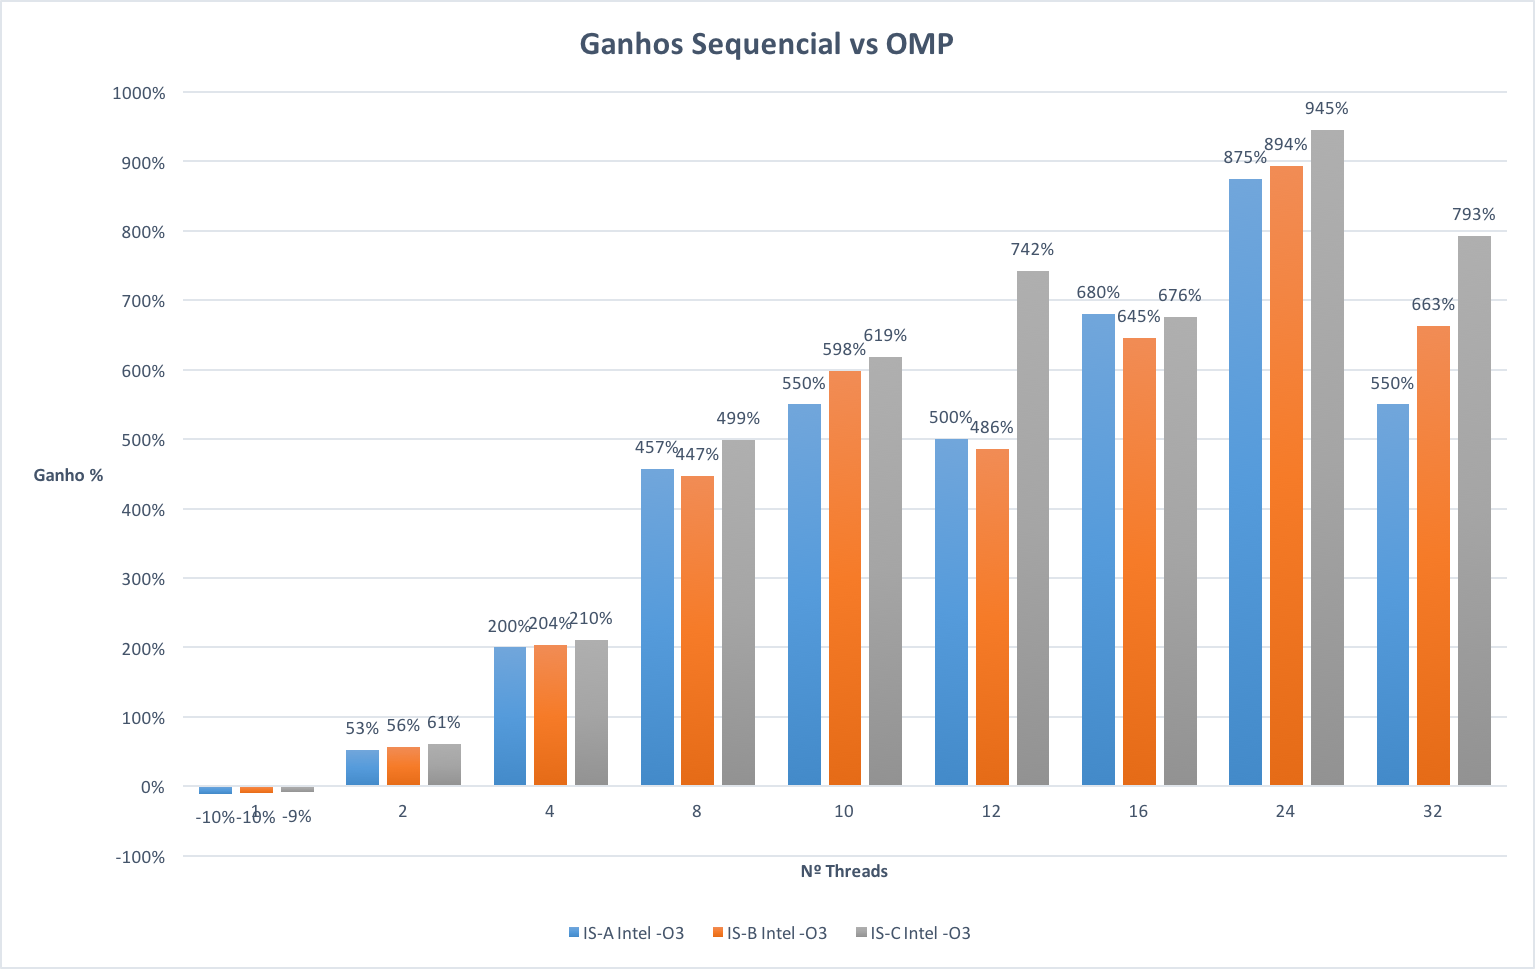
\includegraphics[scale=0.325]{ganhos_seq_vs_omp.png}
\caption{Percentagem de Ganhos Versão Sequencial vs Versão OMP}
\label{fig:ganhos_seq_vs_omp}
\end{figure}

Como podemos verificar no gráfico da figura \ref{fig:ganhos_seq_vs_omp}, os tempos da versão OMP começam mesmo por ter um ganho negativo, isto é, tem um tempo pior que a versão sequencial. Contudo, à medida que vai aumentado o numero de \textit{Threads} os ganhos também vão aumentando, atingindo o seu máximo para 24 \textit{Threads}. Para a classe de dados A, B e C com 24 \textit{Threads} os ganhos são de 875\%, 894\% e 945\% respetivamente, em relação à versão sequencial.
\subsection{Sequencial vs MPI}
Na relação de ganhos entre a versão sequencial e a versão MPI, eu fixei o compilador e as flags, sendo que apresento os ganhos para todas as classes de dados, e para o diferente numero de processos, para o qual efetuei os testes, como pode ser comprovado pela gráfico da figura \ref{fig:ganhos_seq_vs_mpi}.

\begin{figure}[h!]
\centering
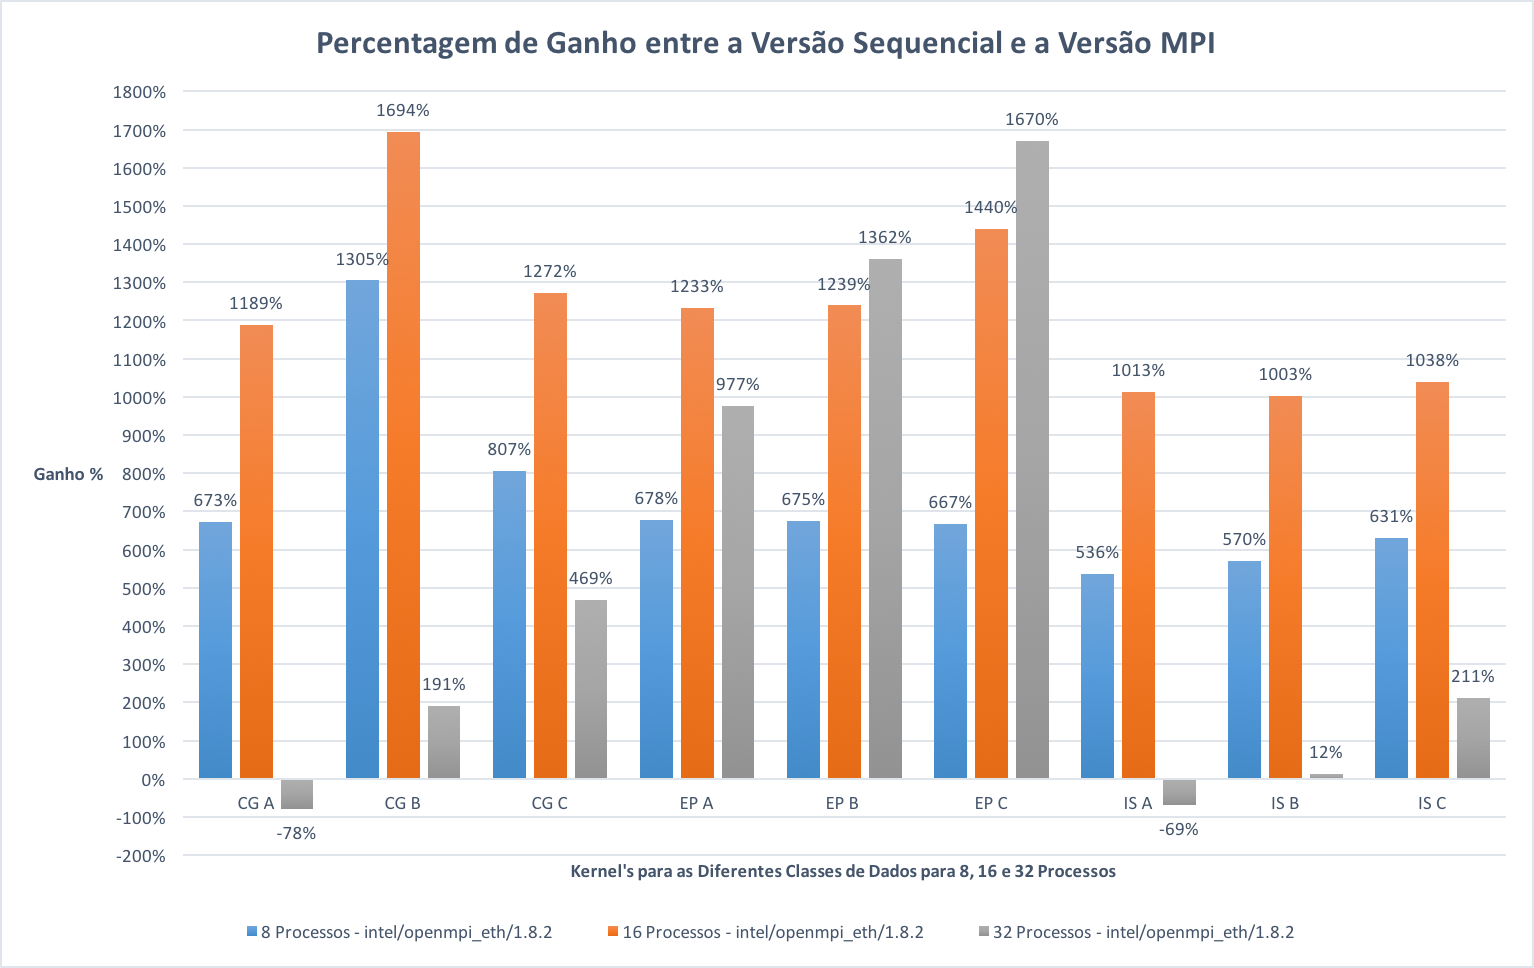
\includegraphics[scale=0.325]{ganhos_seq_vs_mpi.png}
\caption{Percentagem de Ganhos Versão Sequencial vs Versão MPI}
\label{fig:ganhos_seq_vs_mpi}
\end{figure}

Como pode ser analisado pelo gráfico no \textit{Kernel} CG, é com 16 processos que se atinge maior percentagem de ganhos da versão MPI em relação à versão sequencial, tanto para a classe de dados A, como B e como C, apresentando valores de 1189\%, 1695\% e 1272\%. Já no \textit{Kernel} EP a percentagem de ganho da versão MPI em relação à versão sequencial atinge o seu máximo com 32 processos para a classe B e C, com valores de 1392\% e 1670\% e para a classe de dados A atinge o seu máximo com 16 processos com um valor de 1233\%.

Por fim, no \textit{Kernel} IS a percentagem de ganho da versão MPI em relação à versão sequencial, atinge o seu máximo com 16 processos, independentemente da classe de dados, apresentando um valor de 1013\% para a classe de dados A, 1003\% para a classe de dados B e 1038\% para a classe de dados C.

De referir que no caso do \textit{Kernel} CG e do \textit{Kernel} IS, com 32 processos para a classe de dados A, a percentagem de ganho chega a ser negativa, isto é, o tempo de execução da versão MPI é pior que o tempo de execução da versão sequencial.

\section{Utilitários de Monitorização}
No desenvolvimento deste trabalho, aquando de cada teste utilizei uma ferramenta de monitorização, no meu caso \textit{dstat}, para examinar o estado do sistema de operação, neste caso o \textit{Cluster Search}. Estas ferramentas permite-nos visualizar a forma como o sistema é afetado em termos de utilização do \textit{cpu}, da memória e dos discos aquando do aumento gradual da carga de computação.

Como referi, utilizei o comando \textit{dstat} com as seguintes flags:
\begin{itemize}
\item c - ativa as estatísticas do \textit{cpu} (\textit{system}, \textit{user}, \textit{idle}, \textit{wait}, \textit{hardware interrupt} e \textit{software interrupt});
\item d - ativa as estatísticas do disco (\textit{read} e \textit{write});
\item m - ativa as estatísticas de memória (\textit{used}, \textit{buffers}, \textit{cache}, \textit{free}).
\end{itemize}

Nesta secção irei analizar estas estatísticas para um dado \textit{Kernel}, no meu caso para o \textit{Kernel} IS, para o compilador da \textit{Intel} com flag -O3 com a classe de dados C para cada uma das versões, isto é, para a versão sequencial, versão OMP, nas máquinas 431 e para a e versão MPI nas máquinas 641.

\subsection{Versão Sequencial}
Na versão sequencial apenas apresento os gráficos do \textit{dstat} respetivos ao melhor tempo de execusão.

\begin{figure}[h!]
\centering
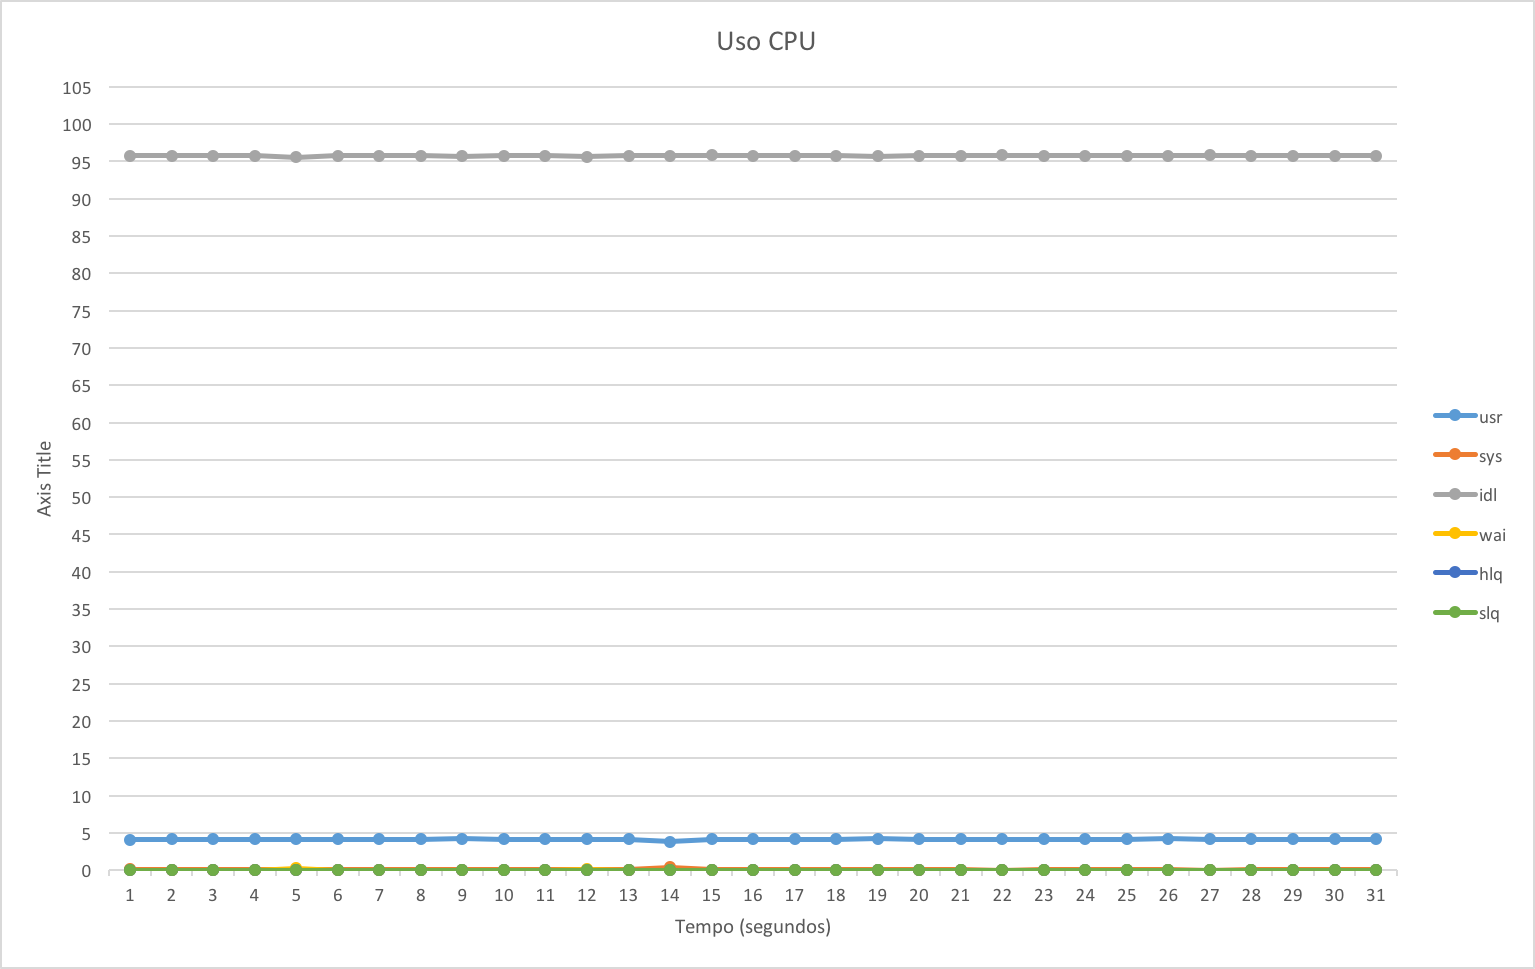
\includegraphics[scale=0.325]{dstat/SER/dstat_seq_cpu.png}
\caption{Percentagem de Uso do CPU}
\label{fig:dstat_seq_cpu}
\end{figure}

\begin{figure}[h!]
\centering
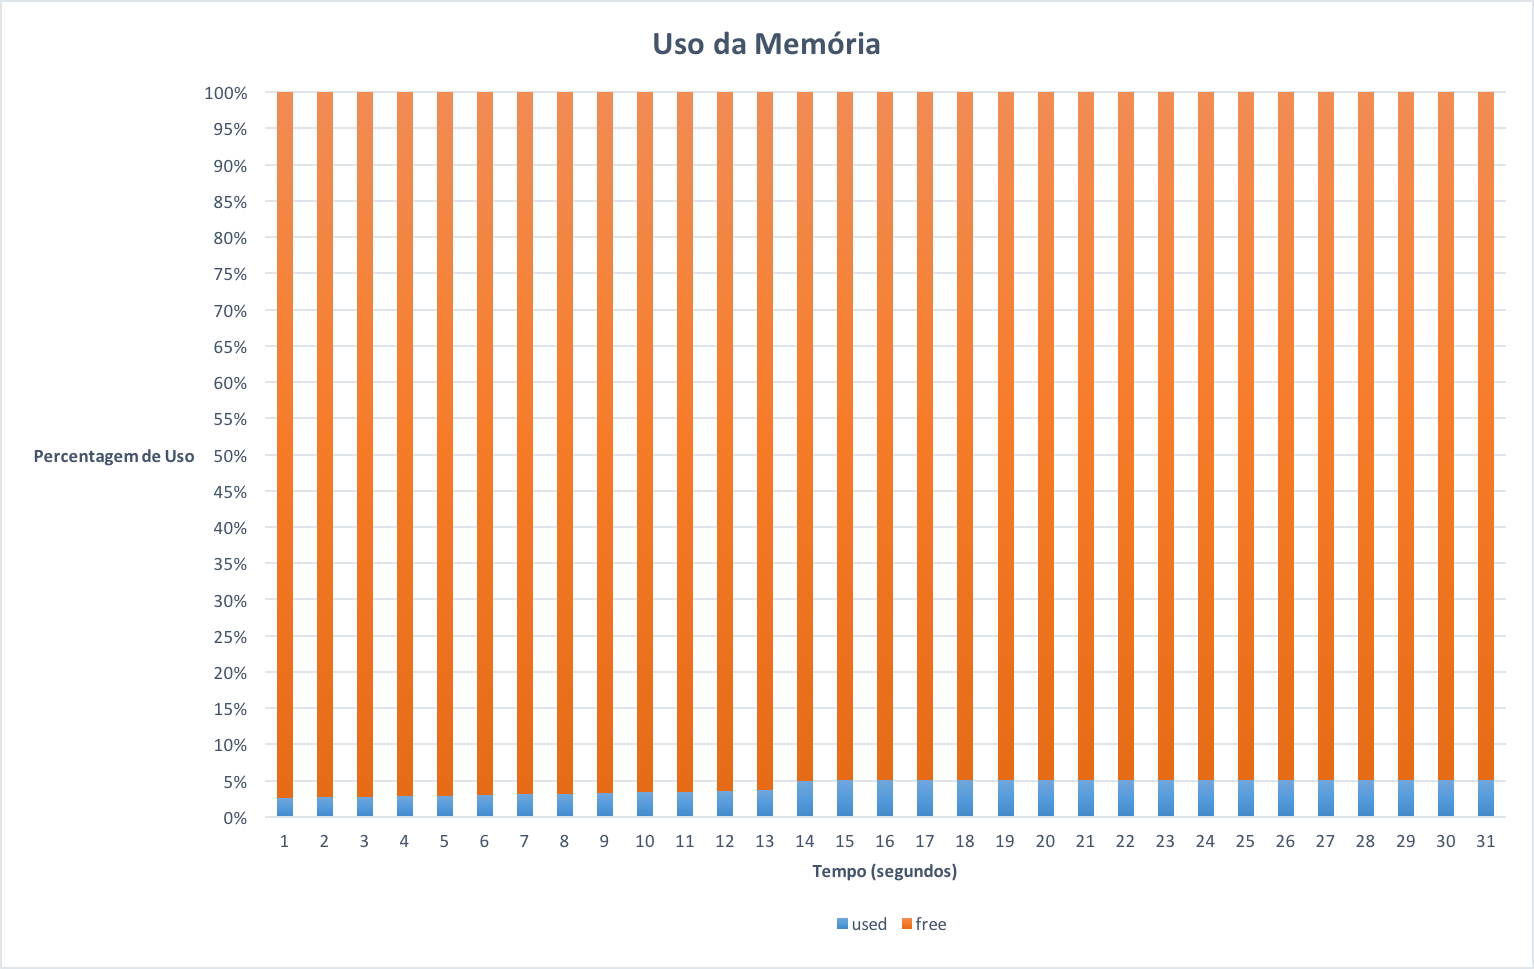
\includegraphics[scale=0.325]{dstat/SER/dstat_seq_memoria.png}
\caption{Percentagem de Uso da Memória}
\label{fig:dstat_seq_memoria}
\end{figure}

\begin{figure}[h!]
\centering
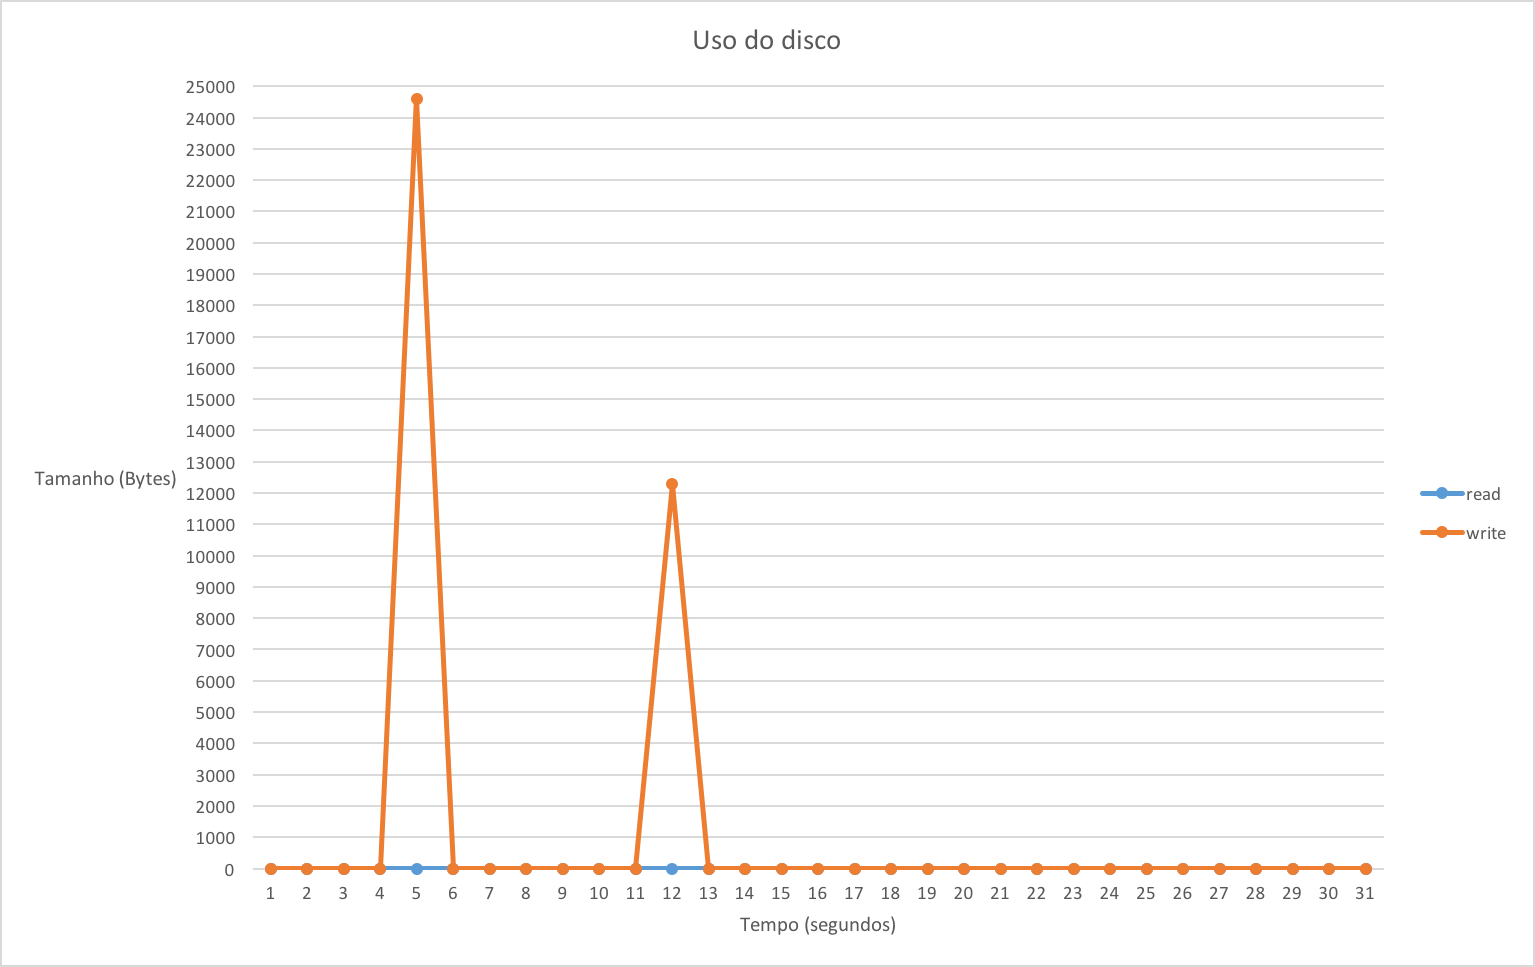
\includegraphics[scale=0.325]{dstat/SER/dstat_seq_disco.png}
\caption{Uso do Disco}
\label{fig:dstat_seq_disco}
\end{figure}

No que toca ao uso do \textit{CPU}, para o \textit{Kernel} IS com a classe de dados C, na máquina 431, na versão sequencial, analisando o gráfico da figura \ref{fig:dstat_seq_cpu} podemos verificar que a percentagem do uso para \textit{user} (\textit{usr}), sobe ligeiramente desde o instante inicial até aos 12 segundos, estabilizando a partir dai nos 5\%, aproximadamente, do uso do \textit{CPU}. A percentagem de uso do \textit{CPU} para \textit{system} (\textit{sys}) em todo o tempo de execução é sempre inferior a 1\%. De referir que o \textit{CPU}, em todo o instante de tempo de execução se encontra desocupado (\textit{idl}) com uma percentagem de cerca de 95\%, daí podemos concluir que o não estamos a tirar o máximo partido do \textit{CPU}, uma vez que a cada instante de tempo, o \textit{Kernel} apenas está a utilizar cerca de 6\% deste.

Na percentagem de uso da memória, analisando o gráfico da figura \ref{fig:dstat_seq_memoria}, verificamos que desde os 14 e até ao fim da execução o \textit{Kernel} está a utilizar cerca de 5\%, aproximadamente, da memória. Sendo que desde o instante inicial, até aos 14 segundos, o \textit{Kernel} vai aumentado o uso da memória ligeiramente. Concluimos assim que o  \textit{Kernel} é \textit{CPU Bound} e não \textit{Memory Bound}. 

Por fim, referente ao uso do disco, ao analisarmos o gráfico da figura \ref{fig:dstat_seq_disco}, verificamos que em todo o instante de execução não leituras (\textit{read}) do disco, sendo que no instante 5 segundos e 12 segundos está a ser escrito (\textit{write}) em disco cerca de 25 KB e 12.5 KB respetivamente.

\subsection{Versão OMP}
Na versão OMP apenas apresento os gráficos do \textit{dstat} respetivos ao melhor tempo de execução para o melhor número de \textit{Threads}, isto é, para o número de \textit{Threads} em que o tempo é menor, neste caso para 24 \textit{Threads}.

\begin{figure}[h!]
\centering
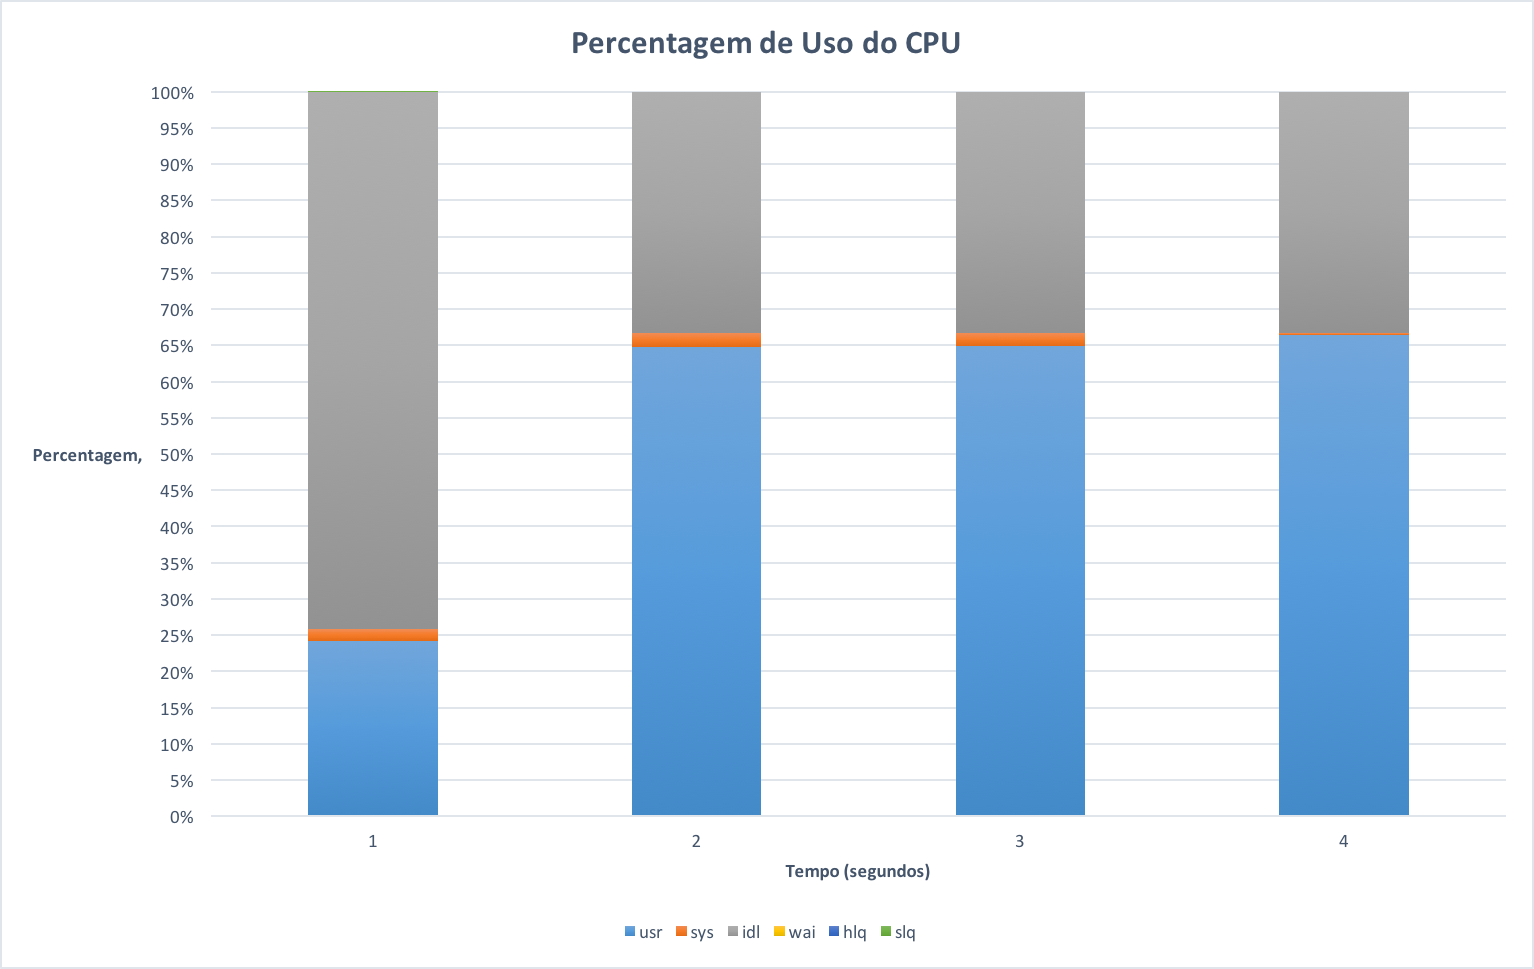
\includegraphics[scale=0.325]{dstat/OMP/dstat_omp_cpu.png}
\caption{Percentagem de Uso do CPU}
\label{fig:dstat_omp_cpu}
\end{figure}

\begin{figure}[h!]
\centering
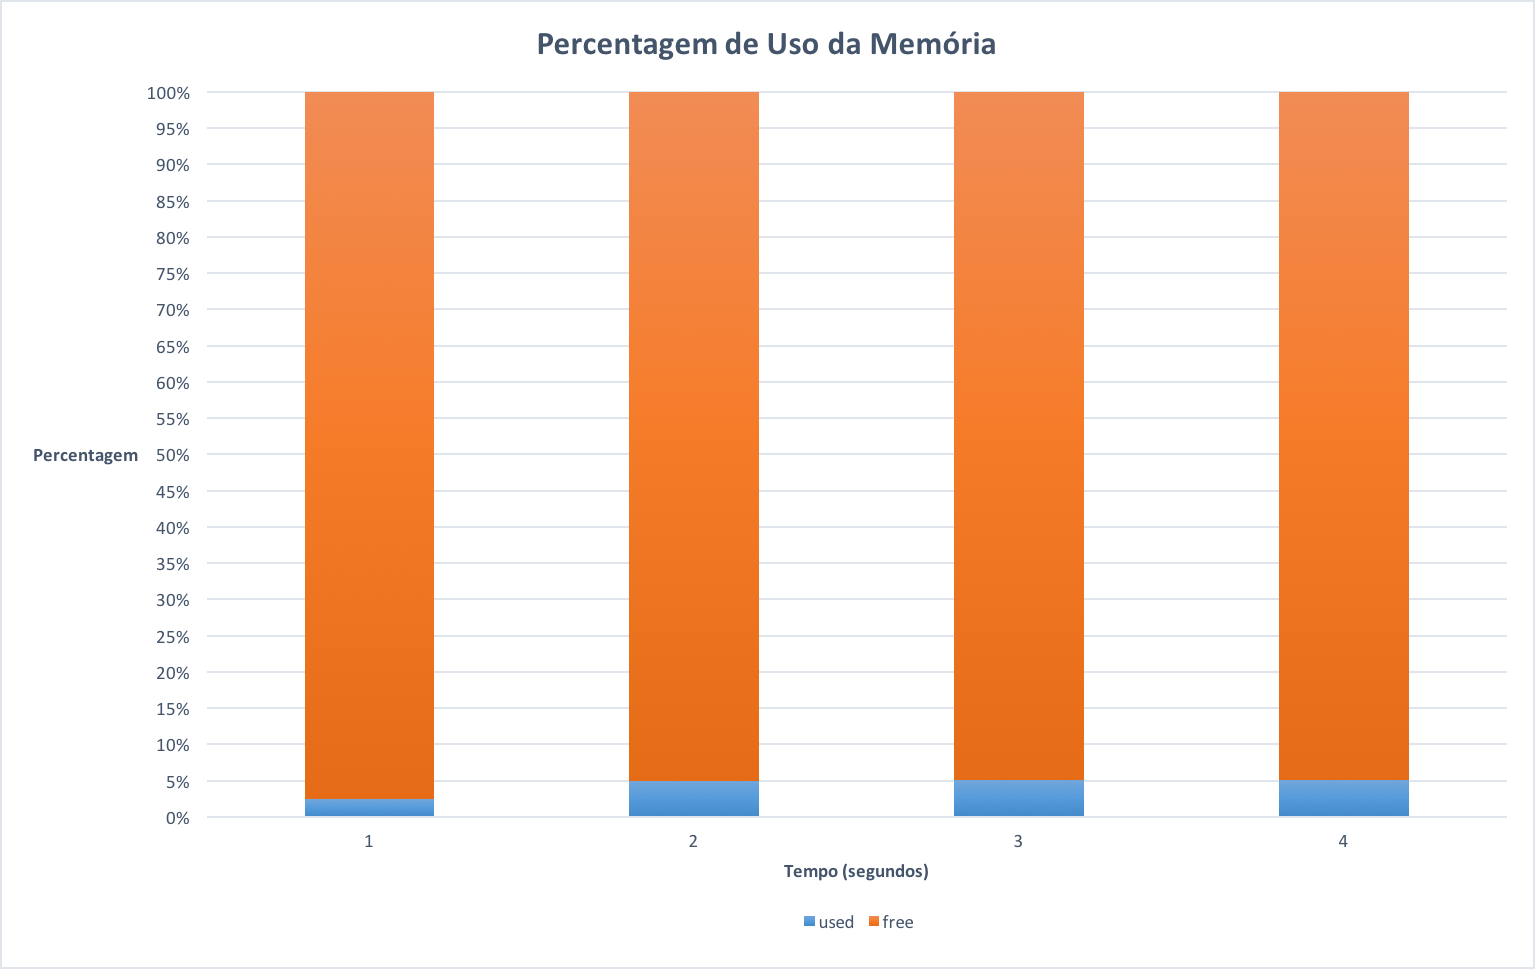
\includegraphics[scale=0.325]{dstat/OMP/dstat_omp_memoria.png}
\caption{Percentagem de Uso da Memória}
\label{fig:dstat_omp_memoria}
\end{figure}

\begin{figure}[h!]
\centering
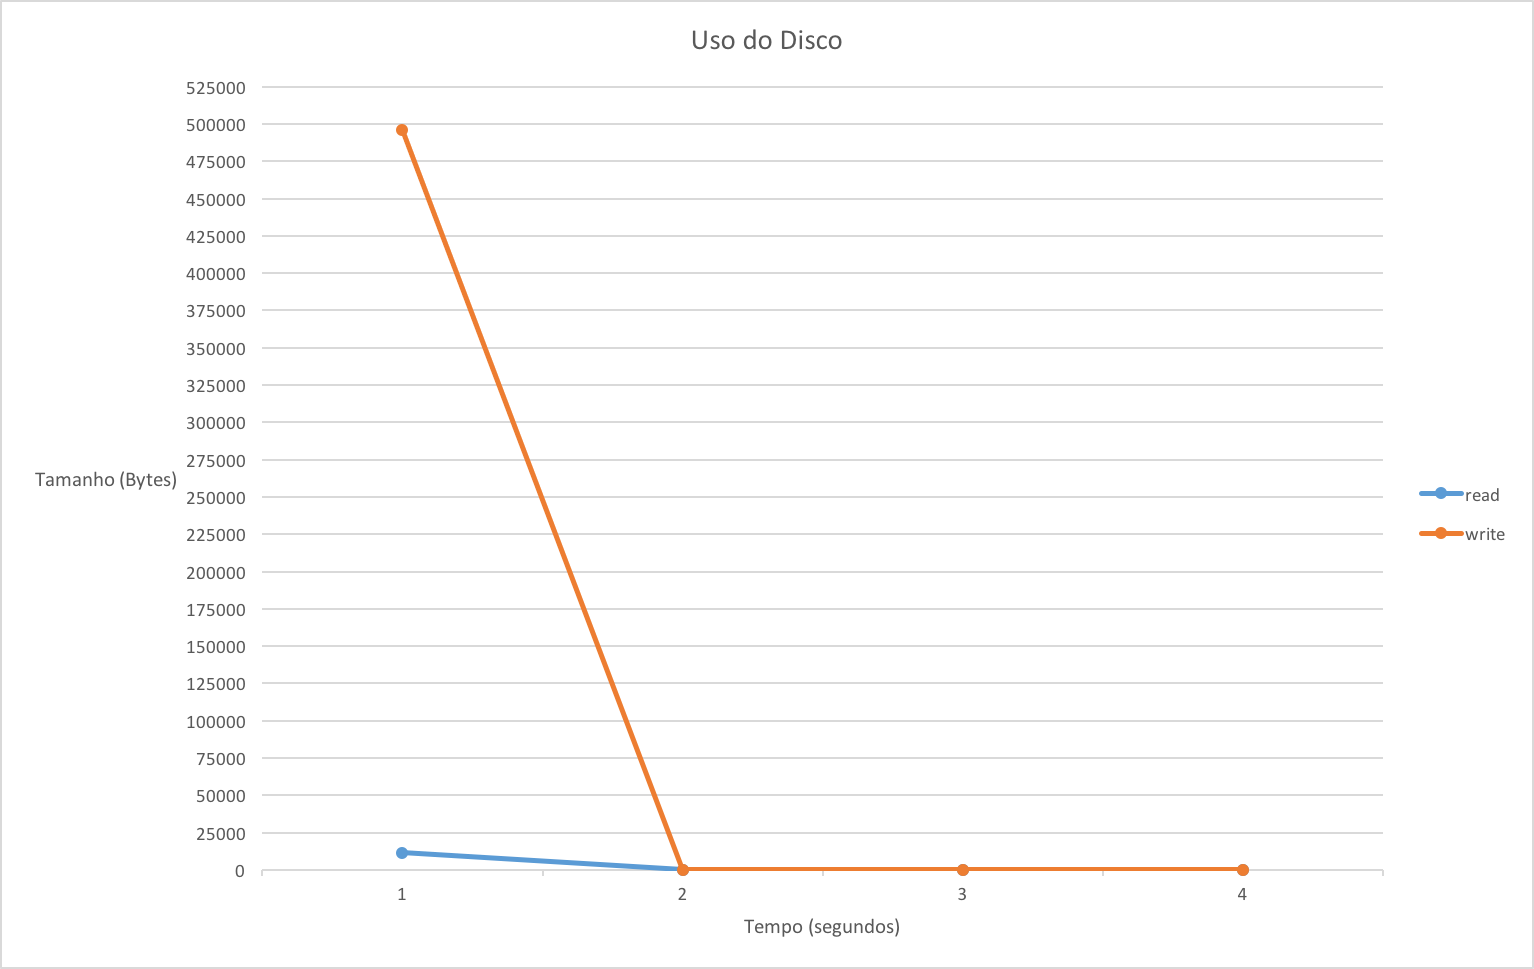
\includegraphics[scale=0.325]{dstat/OMP/dstat_omp_disco.png}
\caption{Uso do Disco}
\label{fig:dstat_omp_disco}
\end{figure}

Analisando o gráfico da figura \ref{fig:dstat_omp_cpu}, referente à percentagem de uso do \textit{CPU}, verificamos que, no primeiro segundo a percentagem de uso do \textit{CPU} para \textit{user} (\textit{usr}) é de cerca de 25\%, a partir do segundo segundo e até final do tempo de execução o uso do \textit{CPU} para \textit{user} (\textit{usr}) mantém-se nos 65\%, aproximadamente. Quanto ao uso do  \textit{CPU} para \textit{system} (\textit{sys}) no primeiro segundo, apresenta um valor inferior a 1\% sendo que a partir dai e até final apresenta um valor de aproximadamente 2\%. Podemos concluir a partir do gráfico que com o paradigma de memória partilhada conseguimos tirar um maior proveito do \textit{CPU} em relação ao sequencial, visto que apresenta uma percentagem de uso mais elevada.

Referente ao uso da memória e analisando o gráfico da figura \ref{fig:dstat_omp_memoria}, verificamos que o \textit{Kernel} no primeiro segundo usa cerca de 2.5\% da memória e a partir do segundo segundo, este utiliza cerca de 5\% da memória, até ao final da execução. Analisando estes resultados podemos concluir que este \textit{Kernel} é \textit{CPU Bound} e não \textit{Memory Bound}, à semelhança do que acontece na versão sequencial.

Para concluir a versão OMP e analisando o gráfico da figura \ref{fig:dstat_omp_disco}, vemos que no primeiro segundo é escrito \textit{write} em disco cerca de 500 KB e lido \textit{read} cerca de 11.5 KB. Nos restantes segundos, até final da execução não há mais leituras nem escritas do disco. 

\subsection{Versão MPI}
Na versão OMP apenas apresento os gráficos do \textit{dstat} respetivos ao melhor tempo de execução para o melhor número de Processos, isto é, para o número de Processos em que o tempo é menor, neste caso com 16 Processos.

\begin{figure}[h!]
\centering
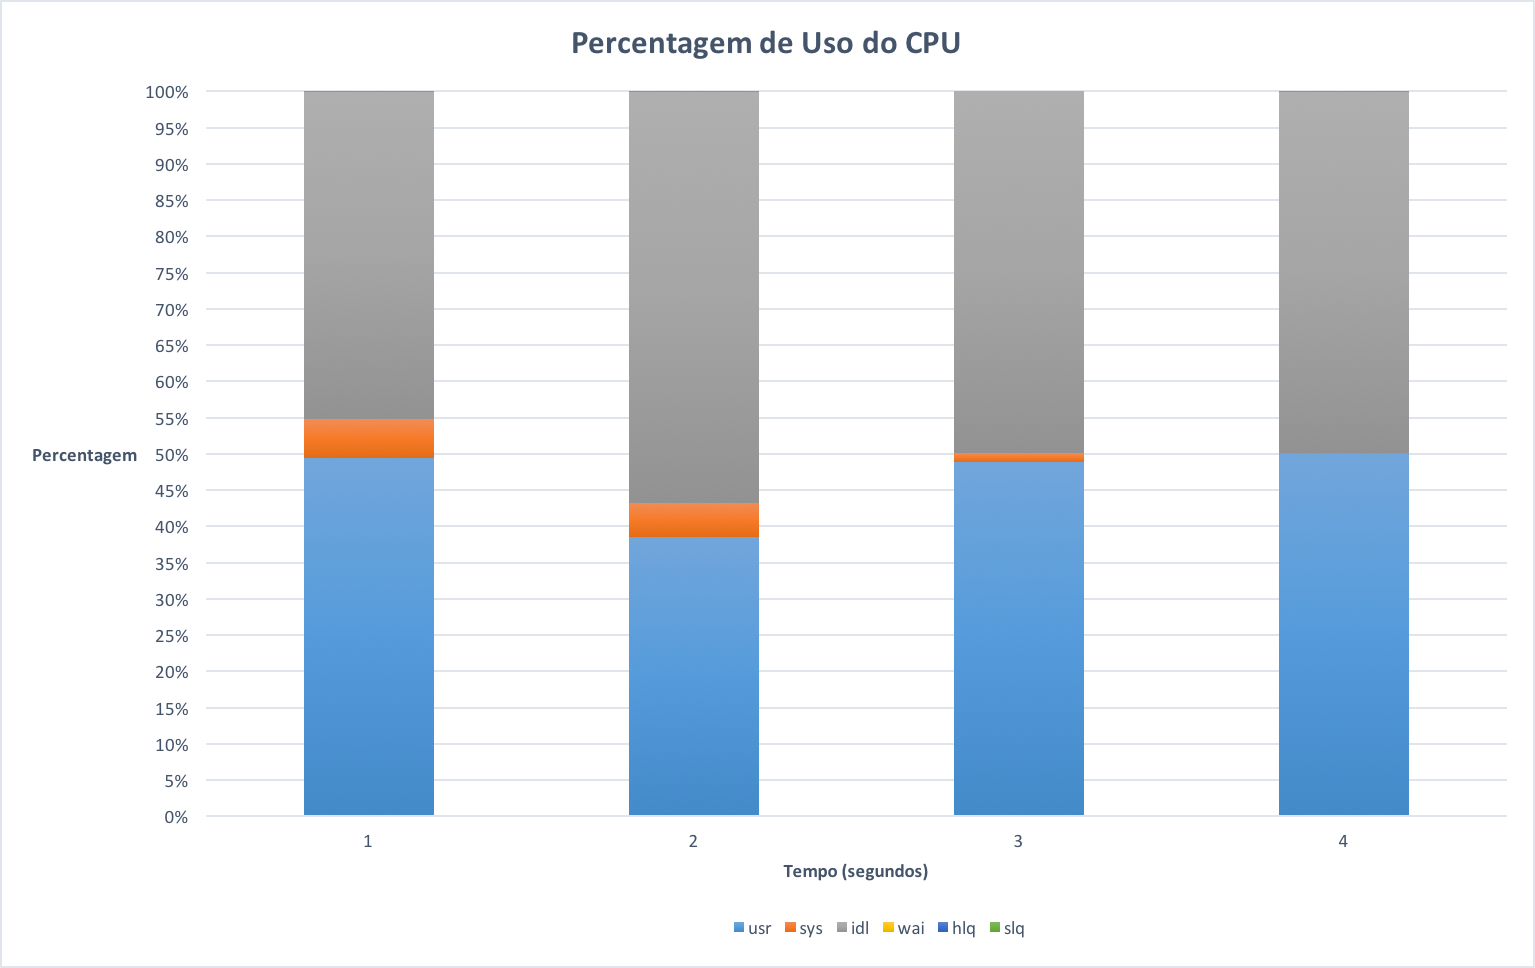
\includegraphics[scale=0.325]{dstat/MPI/dstat_mpi_cpu.png}
\caption{Percentagem de Uso do CPU}
\label{fig:dstat_mpi_cpu}
\end{figure}

\begin{figure}[h!]
\centering
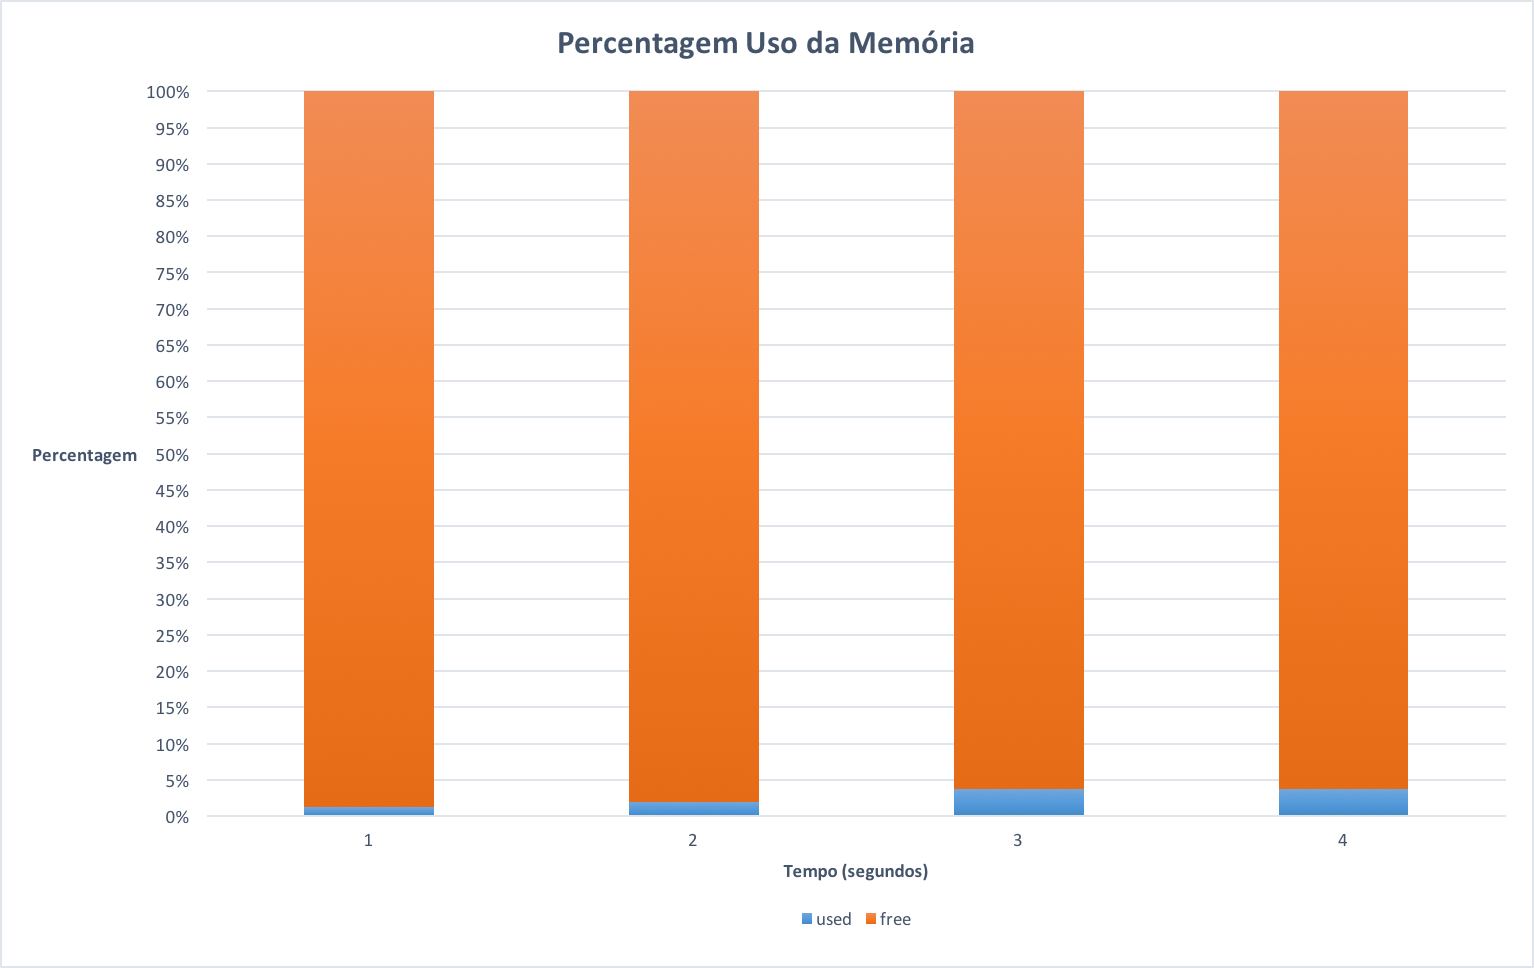
\includegraphics[scale=0.325]{dstat/MPI/dstat_mpi_memoria.png}
\caption{Percentagem de Uso da Memória}
\label{fig:dstat_mpi_memoria}
\end{figure}

\begin{figure}[h!]
\centering
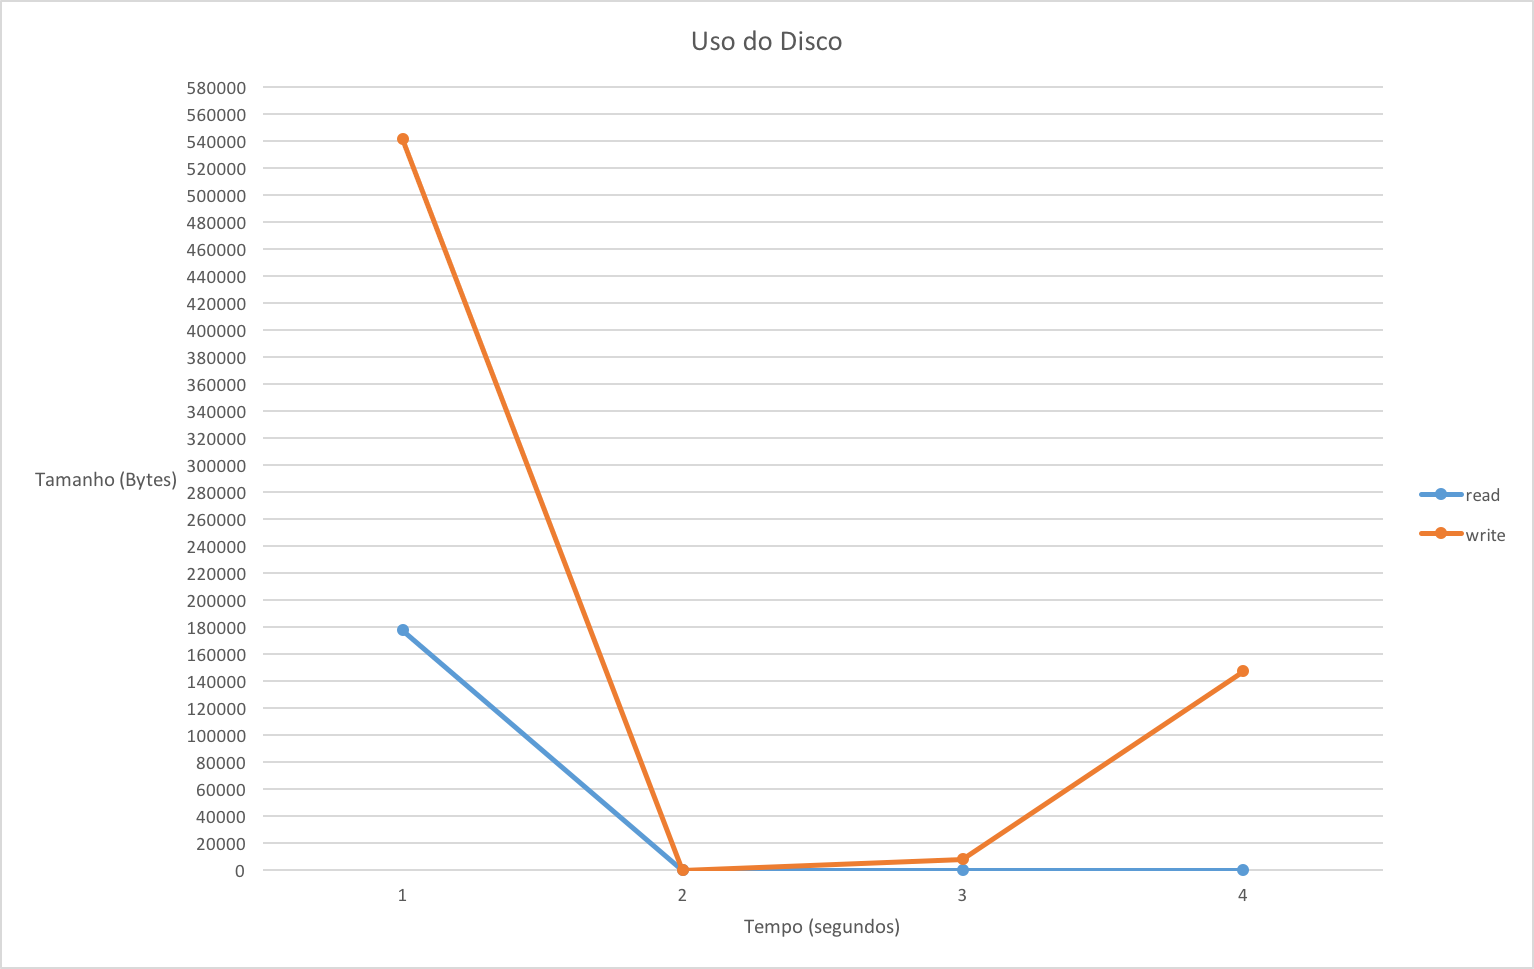
\includegraphics[scale=0.325]{dstat/MPI/dstat_mpi_disco.png}
\caption{Uso do Disco}
\label{fig:dstat_mpi_disco}
\end{figure}

Na versão MPI, quanto ao uso do \textit{CPU} e analisando o gráfico da figura \ref{fig:dstat_mpi_cpu}, verificamos que no primeiro segundo a percentagem de uso para \textit{user} (\textit{usr}) é de cerca de 50\%, sendo que no segundo segundo, baixa para cerca de 38\%, voltando a aumentar nos segundos seguintes, e até final, para cerca de 50\%. Quanto ao uso do \textit{CPU} para \textit{system} (\textit{sys}) no primeiro segundo é de 5\%, baixando nos segundos seguintes, até ao instante final, no qual apresenta um valor inferior a 1\%. De referir que para esta versão MPI em todos os instantes de tempo o \textit{CPU} tem uma percentagem de desocupação (\textit{idl}) de cerca de 50\%.

Nesta versão, a percentagem de uso da memória apresenta padrões semelhantes às versões anteriores (versão sequencial e versão MPI), subindo a cada instante de tempo, mas sempre com valores inferiores a 5\%. Mais uma vez podemos concluir que este \textit{Kernel} é \textit{CPU Bound} e não \textit{Memory Bound}.

Na utilização do disco, verificamos através da analise do gráfico da figura \ref{fig:dstat_mpi_disco}, que no primeiro segundo é escrito (\textit{write}) em disco cerca de 540 KB e lidos (\textit{read}) cerca de 180 KB. No segundo segundo não é escrito nenhum \textit{Byte}, sendo que a partir deste instante não é lido qualquer \textit{Byte}, até final. No terceiro segundo é escrito cerca de 8 KB no disco e no quarto e ultimo segundo é escrito cerca de 150 KB em disco.

\subsection{Análise Geral}
Quanto à analise dos gráficos da ferramenta de monitorização \textit{dstat}, podemos concluir que, na versão OMP é utilizado mais \textit{CPU} em relação às outras versões (versão sequencial e versão MPI), sendo que a versão MPI também apresenta valores razoáveis de utilização do \textit{CPU}. Contudo é com o paradigma de memória distribuída (MPI) que se obtém maiores ganhos, como pode ser comprovado na secção \ref{sec:ganhos}.
Com a análise dos gráficos da percentagem uso de memória, podemos concluir que este \textit{Kernel} é \textit{CPU Bound} e não \textit{Memory Bound}.
Por fim, no que diz respeito ao uso da memória podemos concluir que é na versão MPI que é efetuado maior número de operações de escrita e leitura em disco, como pode ser comprovado pelos gráficos de uso de disco.

\section{Conclusão}
Depois de realizado todos os testes, do tratamento dos resultados e por fim a análise destes, posso concluir de uma maneira geral, que na versão sequencial na máquina 431, os tempos de execução são melhores, quando os \textit{Kernel's} são compilados com o compilador da \textit{Intel}, de notat que á medida que se aumenta os níveis de optimização, o intervalo de tempo de cada gráfico, também vai diminuindo, o que já era de esperar, uma vez que estamos a aumentar as optimizações. Quanto ao número de MOPS, também de uma maneira geral o compilador da \textit{Intel} se mostra o mais eficiente, apresentando valores superiores em relação aos outros compiladores. De notar também que à medida que vamos aumentando os níveis de optimização, o intervalo de valores de cada gráfico vai aumentando, sendo que do nível -O2 para -O3 esse aumento não é muito significativo.

Quanto à versão OMP, podemos concluir que para o \textit{Kernel} IS com um nível de optimização -O2 e -O3 e com a classe de dados C (classe de dados maior), que a versão 4.9.0 e a versão 4.9.3 do compilador da \textit{GNU} são os compiladores mais eficientes, uma vez que é com a execução do \textit{Kernel} compilado com estes compiladores que se encontra o menor tempo, sendo esse valor encontrado na execução do \textit{Kernel} com 24 \textit{Threads}. Quanto ao número de MOPS é com a versão do compilador 4.9.4 do compilador da \textit{GNU} que se encontra o valor mais elevado de MOPS tanto para o nível de optimização -O2 e -O3, sendo esse valor encontrado com 24 \textit{Threads} o que nos permite concluir que é este o melhor compilador, para a obtenção de melhores resultados desta métrica. No que toca aos MOPS/\textit{thread} é com o compilador da \textit{Intel} que se encontra o maior numero de MOPS/\textit{Thread}, sendo este valor encontrado com apenas 1 \textit{Thread}, o que podemos concluir que para a obtenção dos melhores valores desta métrica, é o compilador da \textit{Intel} a melhor escolha. Contudo por uma análise do gráfico dos tempos, podemos concluir que com 1 \textit{Thread} é onde se obtém o pior tempo.

No que toca à versão MPI, podemos concluir que o compilador da \textit{Intel} é o compilador mais eficiente no que toca à obtenção dos melhores tempos, uma vez que de uma maneira geral, é com este compilador, numa execução com 16 processos, mapeados por core, que se obtém os melhores tempos. Quanto ao número de MOPS, também de uma maneira geral é o compilador da \textit{Intel} que é o melhor compilador para a obtenção dos melhores valores desta métrica, uma vez que é com este compilador que, de uma maneira geral, se encontra o maior número de MOPS, sendo estes valores encontrados com 16 processos. Por fim, quanto ao número de MOPS/Processo é o compilador da \textit{Intel} que é o melhor, uma vez que é com este, que encontramos os melhores valores para esta métrica, contudo, ao contrário do que acontece com os tempos e com os MOPS, é com 8 processos que encontramos os melhores valores para esta métrica.

Para finalizar a conclusão da analise dos resultados, relativamente aos ganhos, podemos concluir que o paradigma de memória distribuída (MPI) é o que apresenta melhores tempos de execução relativamente ao sequencial. Na versão MPI os tempos, de uma maneira geral, apresentam valores 1000\% ou mais inferiores à versão sequencial, enquanto na versão OMP o maior ganho é de 945\%.

Referente à realização deste trabalho, efetuei inúmeros testes no \textit{Cluster Search}, para a realização desses testes tive de criar uma forma de automatizar o trabalho, para isso recorri a \textit{Shell Scripts} e ferramentas de escalonamento de tarefas, como o PBS. Depois de efetuados os testes, tive de processar os dados de forma a criar gráficos que exprimissem os meus resultados, para isso usei ferramentas de processamento de linguagens como é o caso do \textit{gawk} e do \textit{grep}, por fim, depois de ter todos os dados organizados, recorri ao excel para a geração dos gráficos. 

Este trabalho permitiu-me ambientar de uma forma mais objetiva num ambiente de \textit{clustering}, sendo que passei por algumas dificuldades principalmente na execução dos testes para a versão MPI, dificuldades essas que não foram totalmente ultrapassadas, pelo menos na execução em \textit{Myrinet}. Para alem dessas dificuldades, apesar de ter automatizado grande parte do trabalho com as \textit{scripts}, penso que perdi demasiado tempo na criação dos gráficos, uma vez que os fiz todos à mão e não era esse o objetivo. Contudo, faço um balanço positivo da maior parte do trabalho, sendo que, como trabalho futuro pretendo aperfeiçoar principalmente o meu processo de automatização, de forma a não perder demasiado tempo em algumas partes, bem como conseguir efetuar todos os testes que defini ao inicio. 

% An example of a floating figure using the graphicx package.
% Note that \label must occur AFTER (or within) \caption.
% For figures, \caption should occur after the \includegraphics.
% Note that IEEEtran v1.7 and later has special internal code that
% is designed to preserve the operation of \label within \caption
% even when the captionsoff option is in effect. However, because
% of issues like this, it may be the safest practice to put all your
% \label just after \caption rather than within \caption{}.
%
% Reminder: the "draftcls" or "draftclsnofoot", not "draft", class
% option should be used if it is desired that the figures are to be
% displayed while in draft mode.
%
%\begin{figure}[!t]
%\centering
%\includegraphics[width=2.5in]{myfigure}
% where an .eps filename suffix will be assumed under latex, 
% and a .pdf suffix will be assumed for pdflatex; or what has been declared
% via \DeclareGraphicsExtensions.
%\caption{Simulation results for the network.}
%\label{fig_sim}
%\end{figure}

% Note that the IEEE typically puts floats only at the top, even when this
% results in a large percentage of a column being occupied by floats.


% An example of a double column floating figure using two subfigures.
% (The subfig.sty package must be loaded for this to work.)
% The subfigure \label commands are set within each subfloat command,
% and the \label for the overall figure must come after \caption.
% \hfil is used as a separator to get equal spacing.
% Watch out that the combined width of all the subfigures on a 
% line do not exceed the text width or a line break will occur.
%
%\begin{figure*}[!t]
%\centering
%\subfloat[Case I]{\includegraphics[width=2.5in]{box}%
%\label{fig_first_case}}
%\hfil
%\subfloat[Case II]{\includegraphics[width=2.5in]{box}%
%\label{fig_second_case}}
%\caption{Simulation results for the network.}
%\label{fig_sim}
%\end{figure*}
%
% Note that often IEEE papers with subfigures do not employ subfigure
% captions (using the optional argument to \subfloat[]), but instead will
% reference/describe all of them (a), (b), etc., within the main caption.
% Be aware that for subfig.sty to generate the (a), (b), etc., subfigure
% labels, the optional argument to \subfloat must be present. If a
% subcaption is not desired, just leave its contents blank,
% e.g., \subfloat[].


% An example of a floating table. Note that, for IEEE style tables, the
% \caption command should come BEFORE the table and, given that table
% captions serve much like titles, are usually capitalized except for words
% such as a, an, and, as, at, but, by, for, in, nor, of, on, or, the, to
% and up, which are usually not capitalized unless they are the first or
% last word of the caption. Table text will default to \footnotesize as
% the IEEE normally uses this smaller font for tables.
% The \label must come after \caption as always.
%
%\begin{table}[!t]
%% increase table row spacing, adjust to taste
%\renewcommand{\arraystretch}{1.3}
% if using array.sty, it might be a good idea to tweak the value of
% \extrarowheight as needed to properly center the text within the cells
%\caption{An Example of a Table}
%\label{table_example}
%\centering
%% Some packages, such as MDW tools, offer better commands for making tables
%% than the plain LaTeX2e tabular which is used here.
%\begin{tabular}{|c||c|}
%\hline
%One & Two\\
%\hline
%Three & Four\\
%\hline
%\end{tabular}
%\end{table}


% Note that the IEEE does not put floats in the very first column
% - or typically anywhere on the first page for that matter. Also,
% in-text middle ("here") positioning is typically not used, but it
% is allowed and encouraged for Computer Society conferences (but
% not Computer Society journals). Most IEEE journals/conferences use
% top floats exclusively. 
% Note that, LaTeX2e, unlike IEEE journals/conferences, places
% footnotes above bottom floats. This can be corrected via the
% \fnbelowfloat command of the stfloats package.




% trigger a \newpage just before the given reference
% number - used to balance the columns on the last page
% adjust value as needed - may need to be readjusted if
% the document is modified later
%\IEEEtriggeratref{8}
% The "triggered" command can be changed if desired:
%\IEEEtriggercmd{\enlargethispage{-5in}}

% references section

% can use a bibliography generated by BibTeX as a .bbl file
% BibTeX documentation can be easily obtained at:
% http://mirror.ctan.org/biblio/bibtex/contrib/doc/
% The IEEEtran BibTeX style support page is at:
% http://www.michaelshell.org/tex/ieeetran/bibtex/
%\bibliographystyle{IEEEtran}
% argument is your BibTeX string definitions and bibliography database(s)
%\bibliography{IEEEabrv,../bib/paper}
%
% <OR> manually copy in the resultant .bbl file
% set second argument of \begin to the number of references
% (used to reserve space for the reference number labels box)

\bibliographystyle{abbrv}
\bibliography{references}

\appendix

\section{Gráficos de Tempos e MOPS para as Máquinas 641 para a versão sequencial}
\label{appendix:641_seq}

\begin{figure}[h!]
\centering
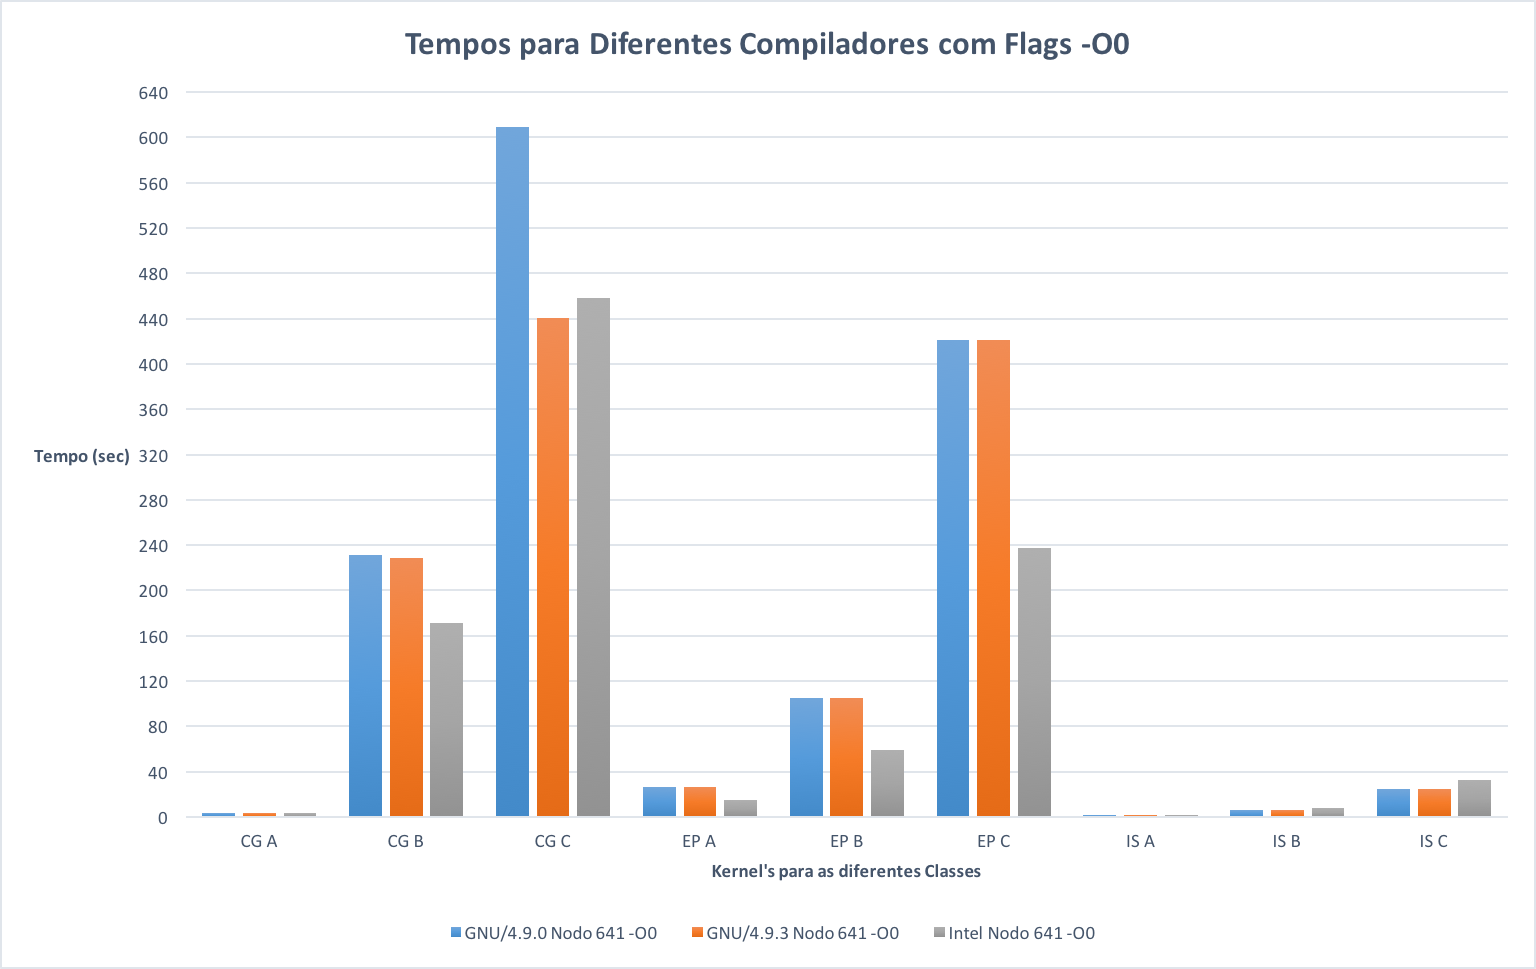
\includegraphics[scale=0.325]{SER/tempos_dif_comp_O0_nodo_641.png}
\caption{Tempos para Diferentes Compiladores com Flags -O0}
\end{figure}

\begin{figure}[h!]
\centering
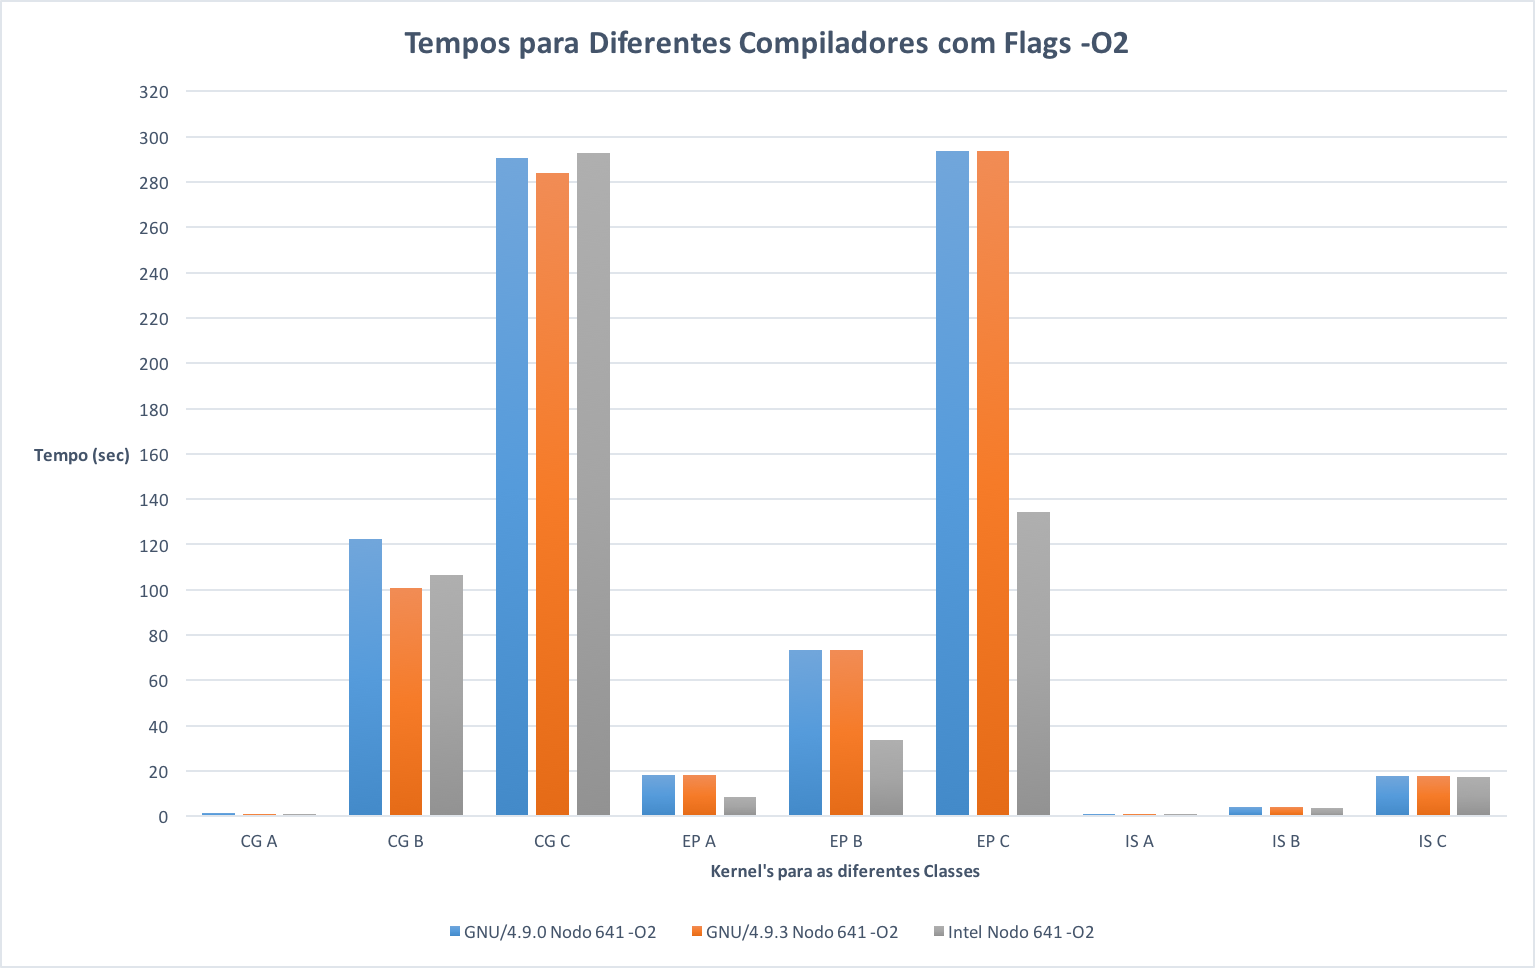
\includegraphics[scale=0.325]{SER/tempos_dif_comp_O2_nodo_641.png}
\caption{Tempos para Diferentes Compiladores com Flags -O2}
\end{figure}

\begin{figure}[h!]
\centering
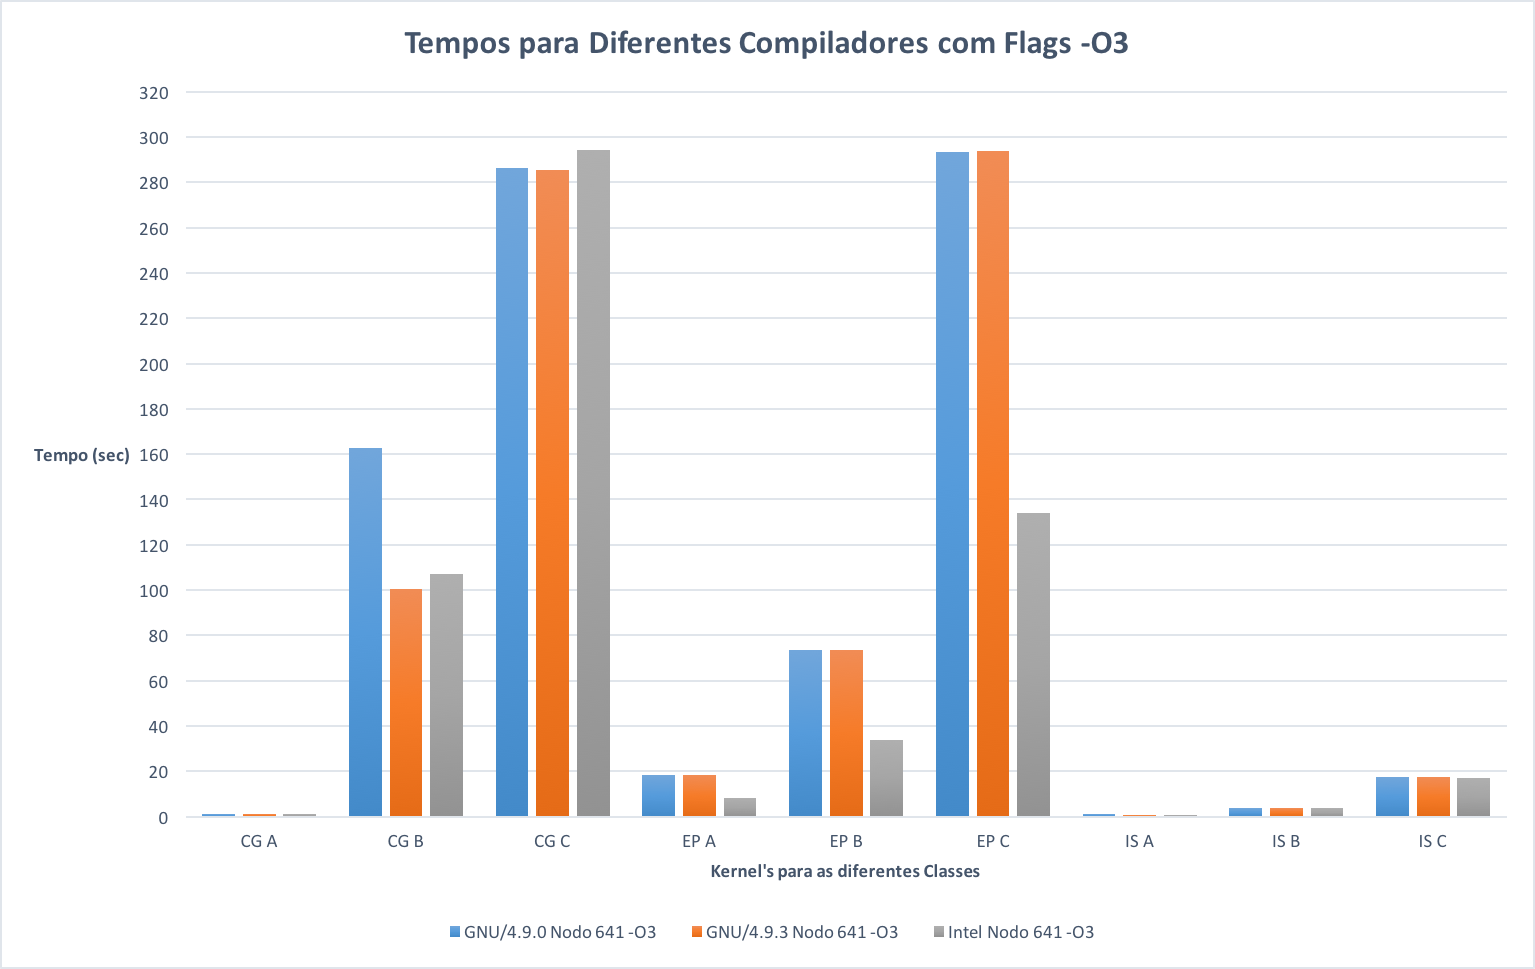
\includegraphics[scale=0.325]{SER/tempos_dif_comp_O3_nodo_641.png}
\caption{Tempos para Diferentes Compiladores com Flags -O3}
\end{figure}

\begin{figure}[h!]
\centering
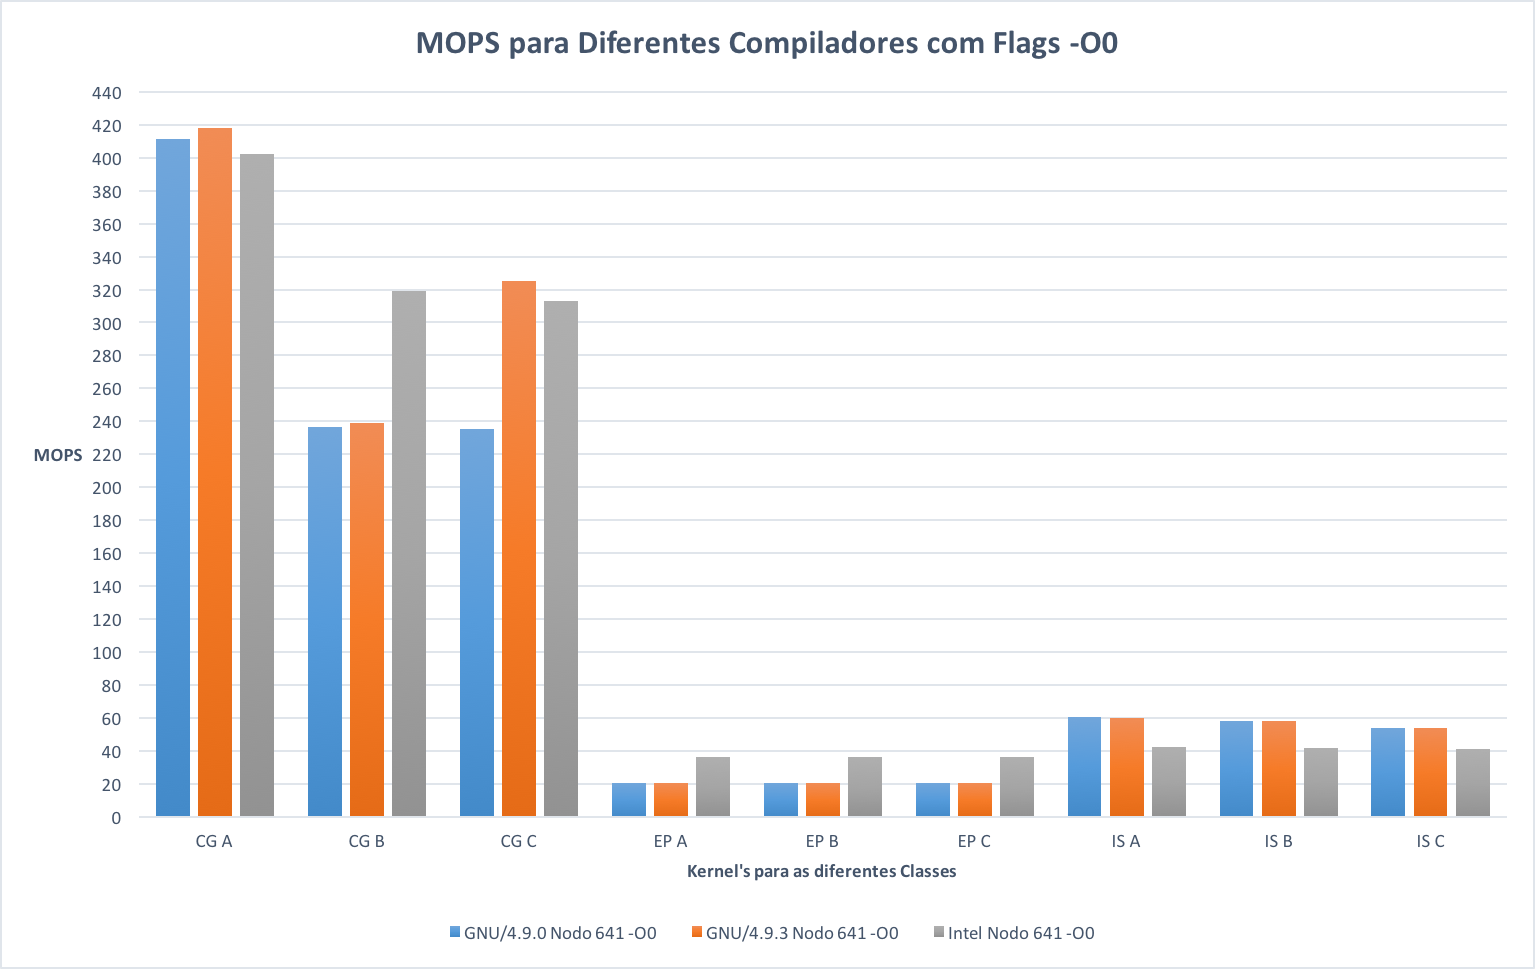
\includegraphics[scale=0.325]{SER/mops_dif_comp_O0_nodo_641.png}
\caption{MOPS para Diferentes Compiladores com Flags -O0}
\end{figure}

\begin{figure}[h!]
\centering
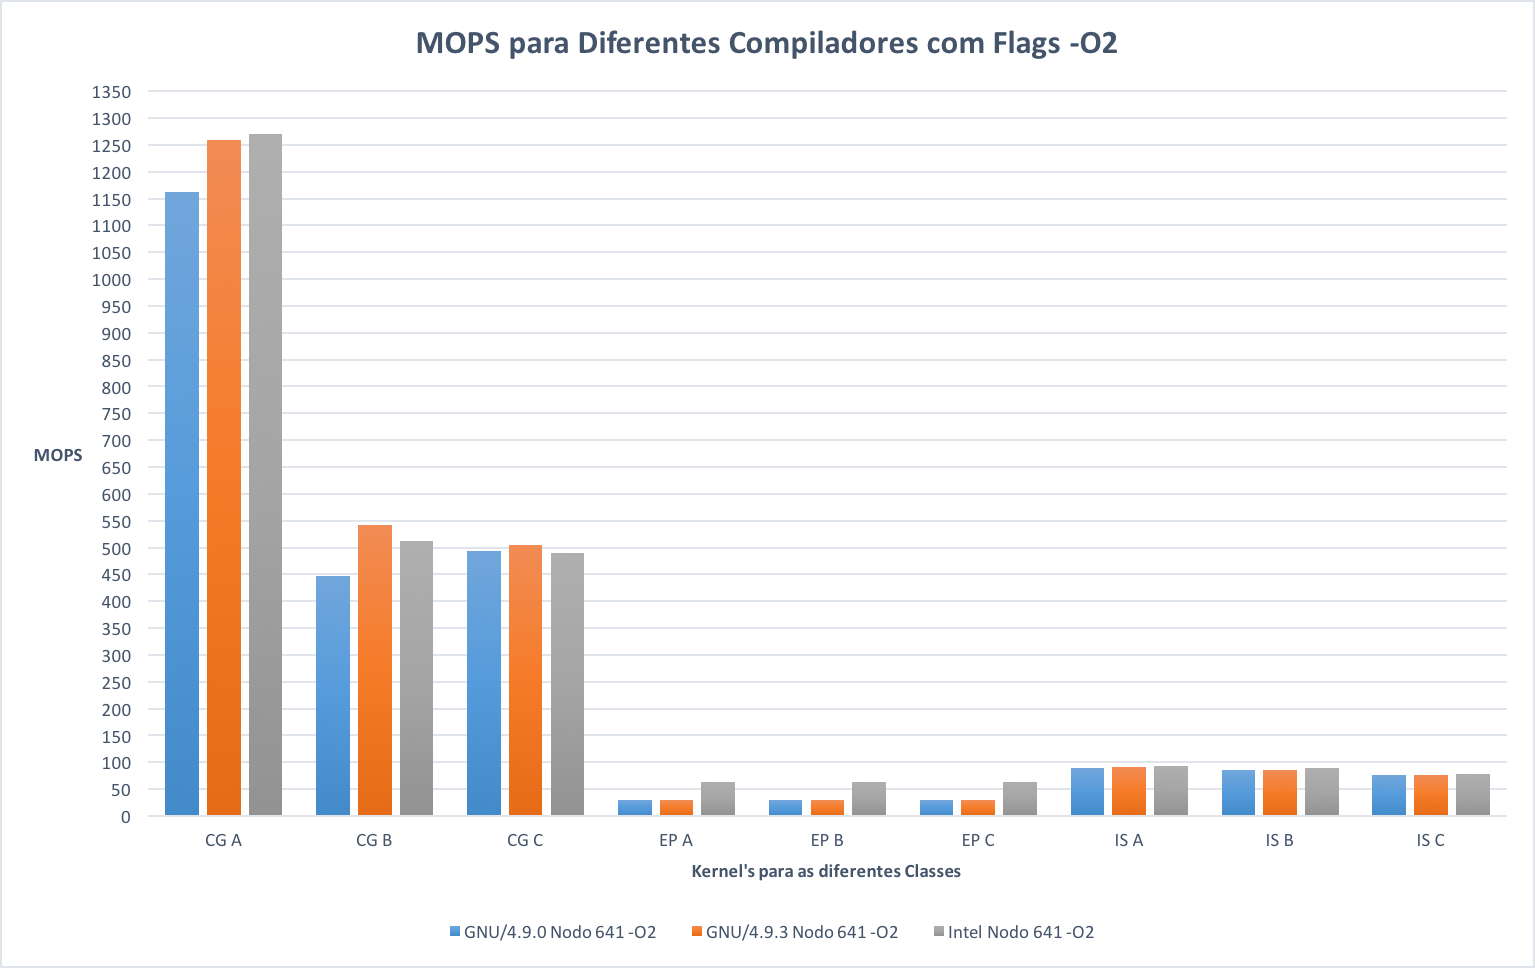
\includegraphics[scale=0.325]{SER/mops_dif_comp_O2_nodo_641.png}
\caption{MOPS para Diferentes Compiladores com Flags -O2}
\end{figure}

\begin{figure}[h!]
\centering
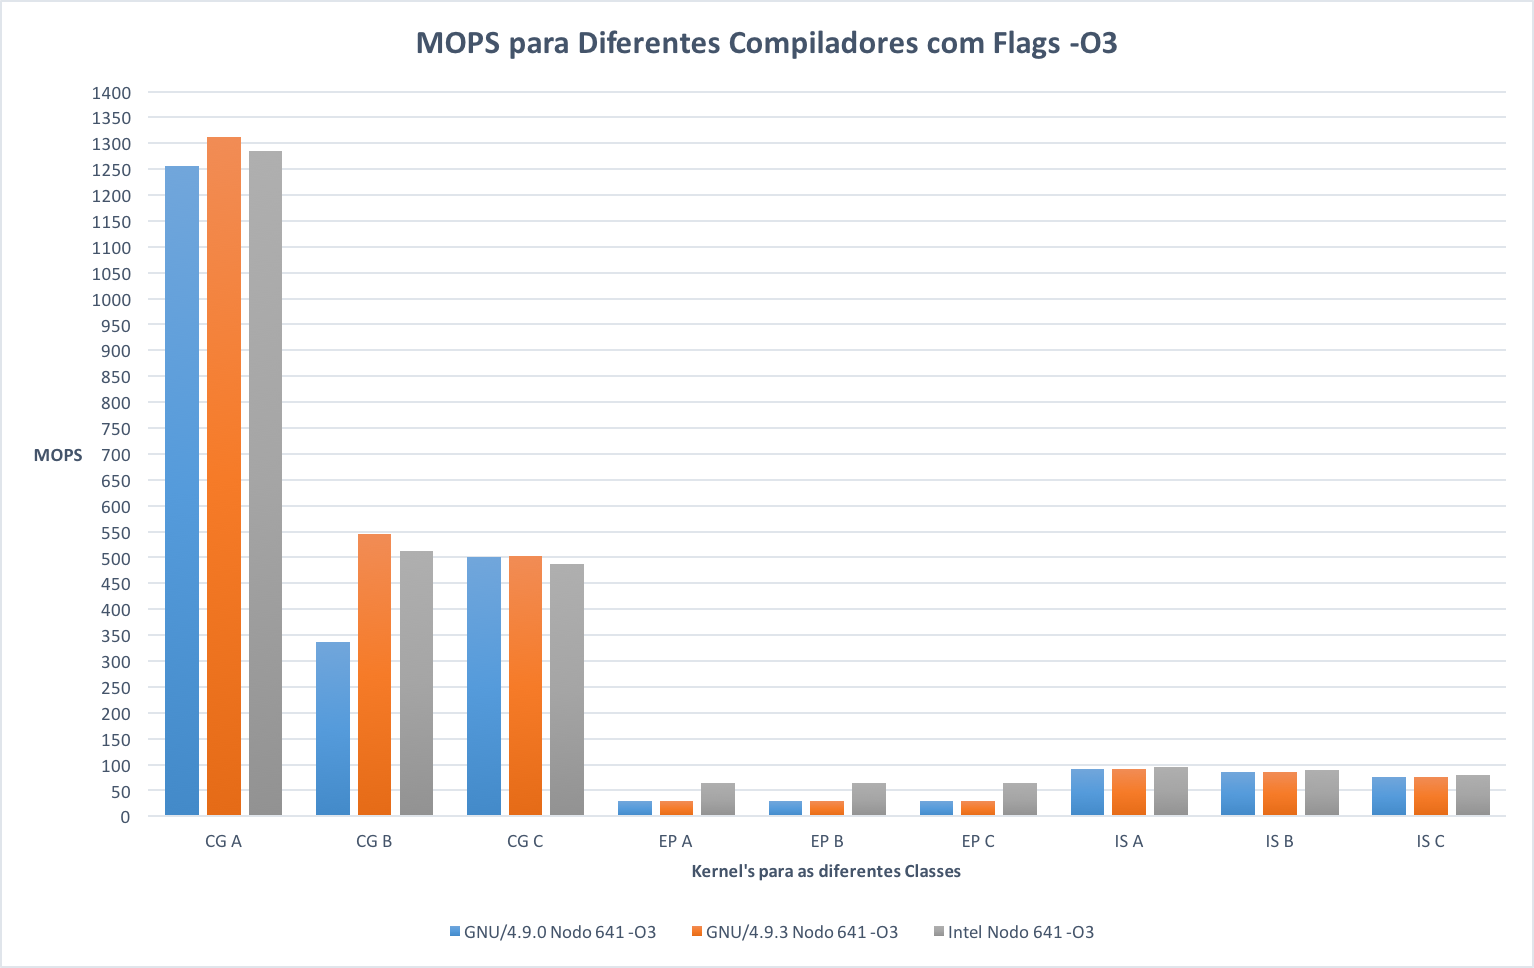
\includegraphics[scale=0.325]{SER/mops_dif_comp_O3_nodo_641.png}
\caption{MOPS para Diferentes Compiladores com Flags -O3}
\end{figure}

\section{Gráficos de Tempos, MOPS e MOPS/\textit{Thread} para as Máquinas 641 para a versão OMP}
\label{appendix:641_omp}

\begin{figure}[h!]
\centering
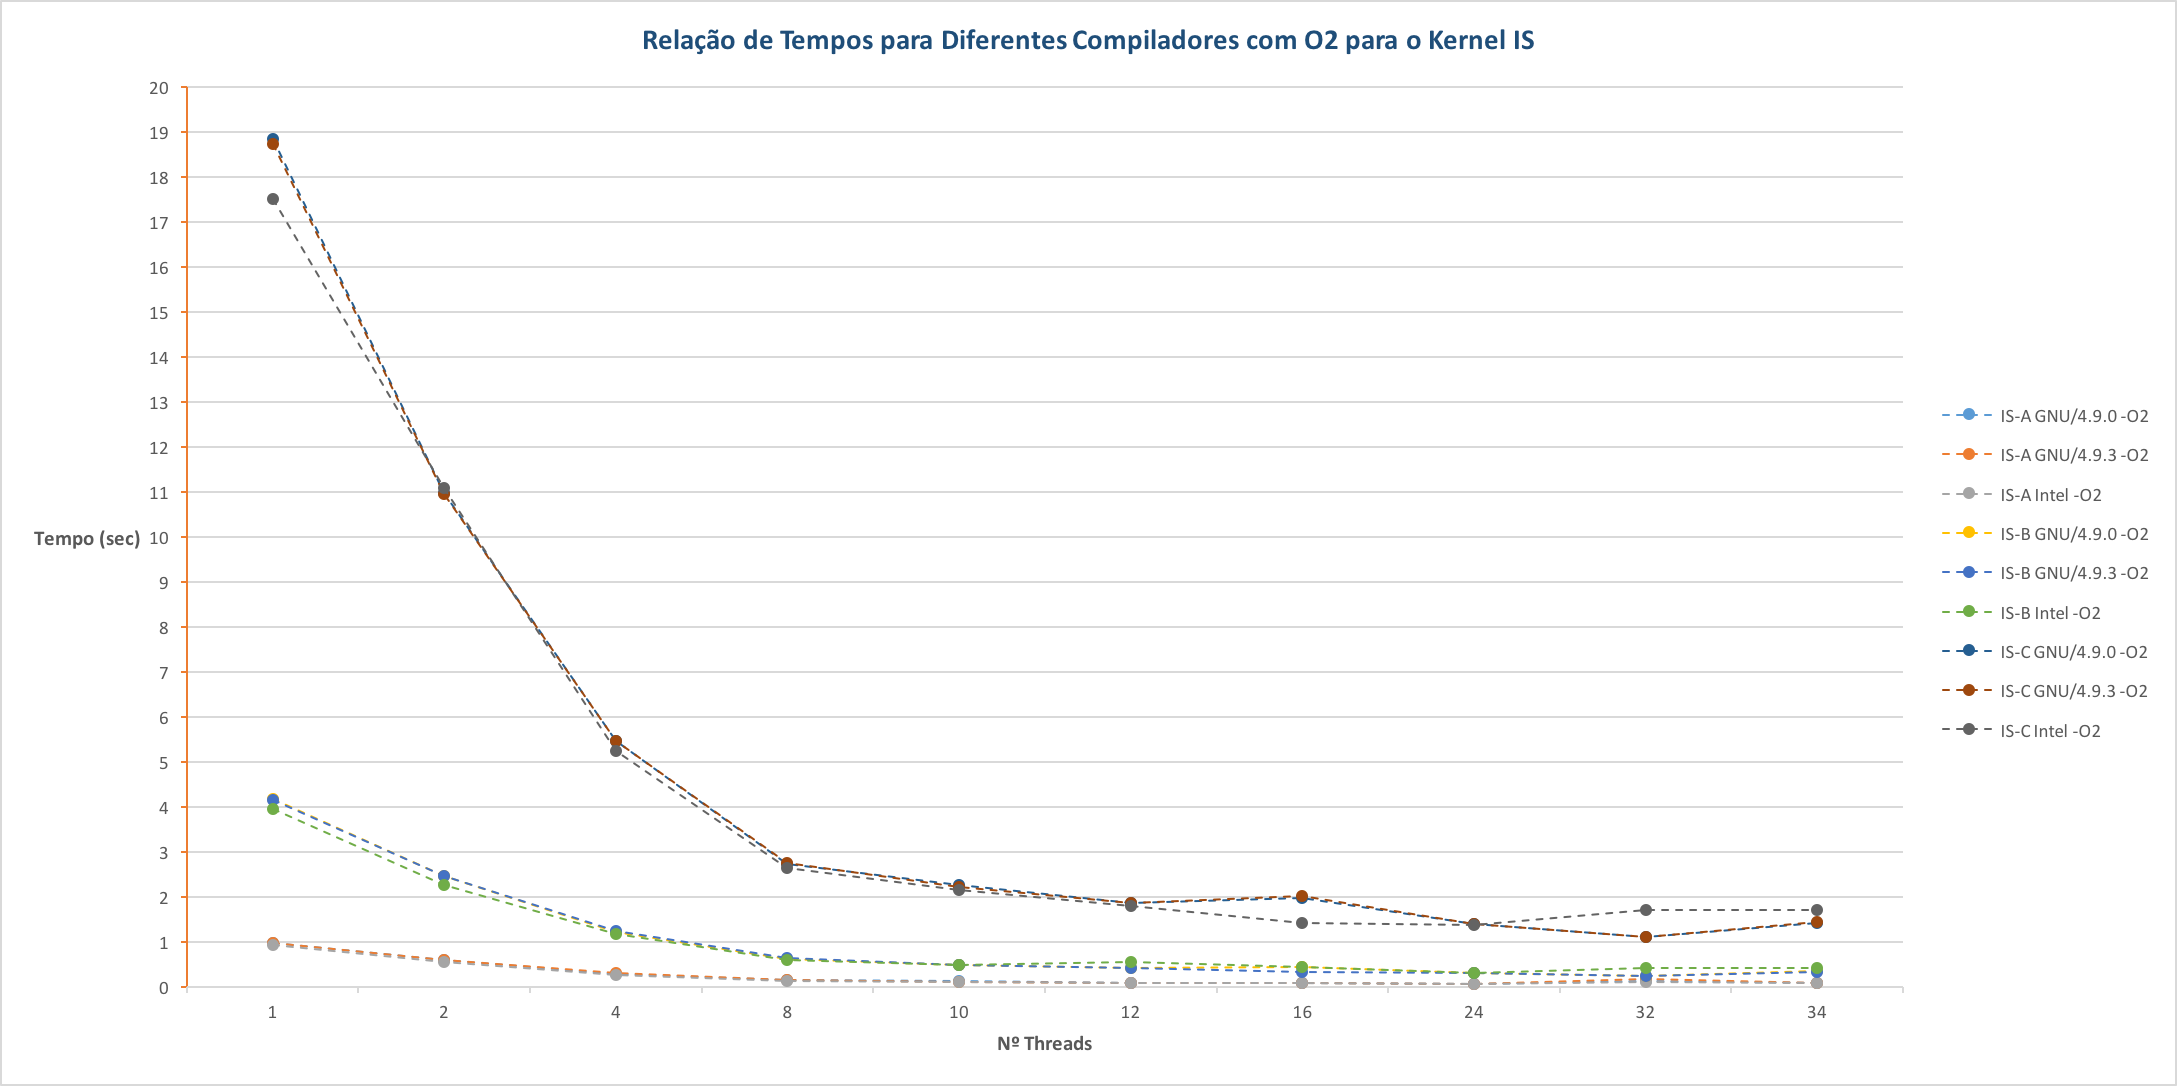
\includegraphics[scale=0.25]{OMP/tempos_dif_comp-O2_IS_nodo-641.png}
\caption{Tempos para Diferentes Compiladores com Flags -O2 para o \textit{Kernel} IS}
\end{figure}

\begin{figure}[h!]
\centering
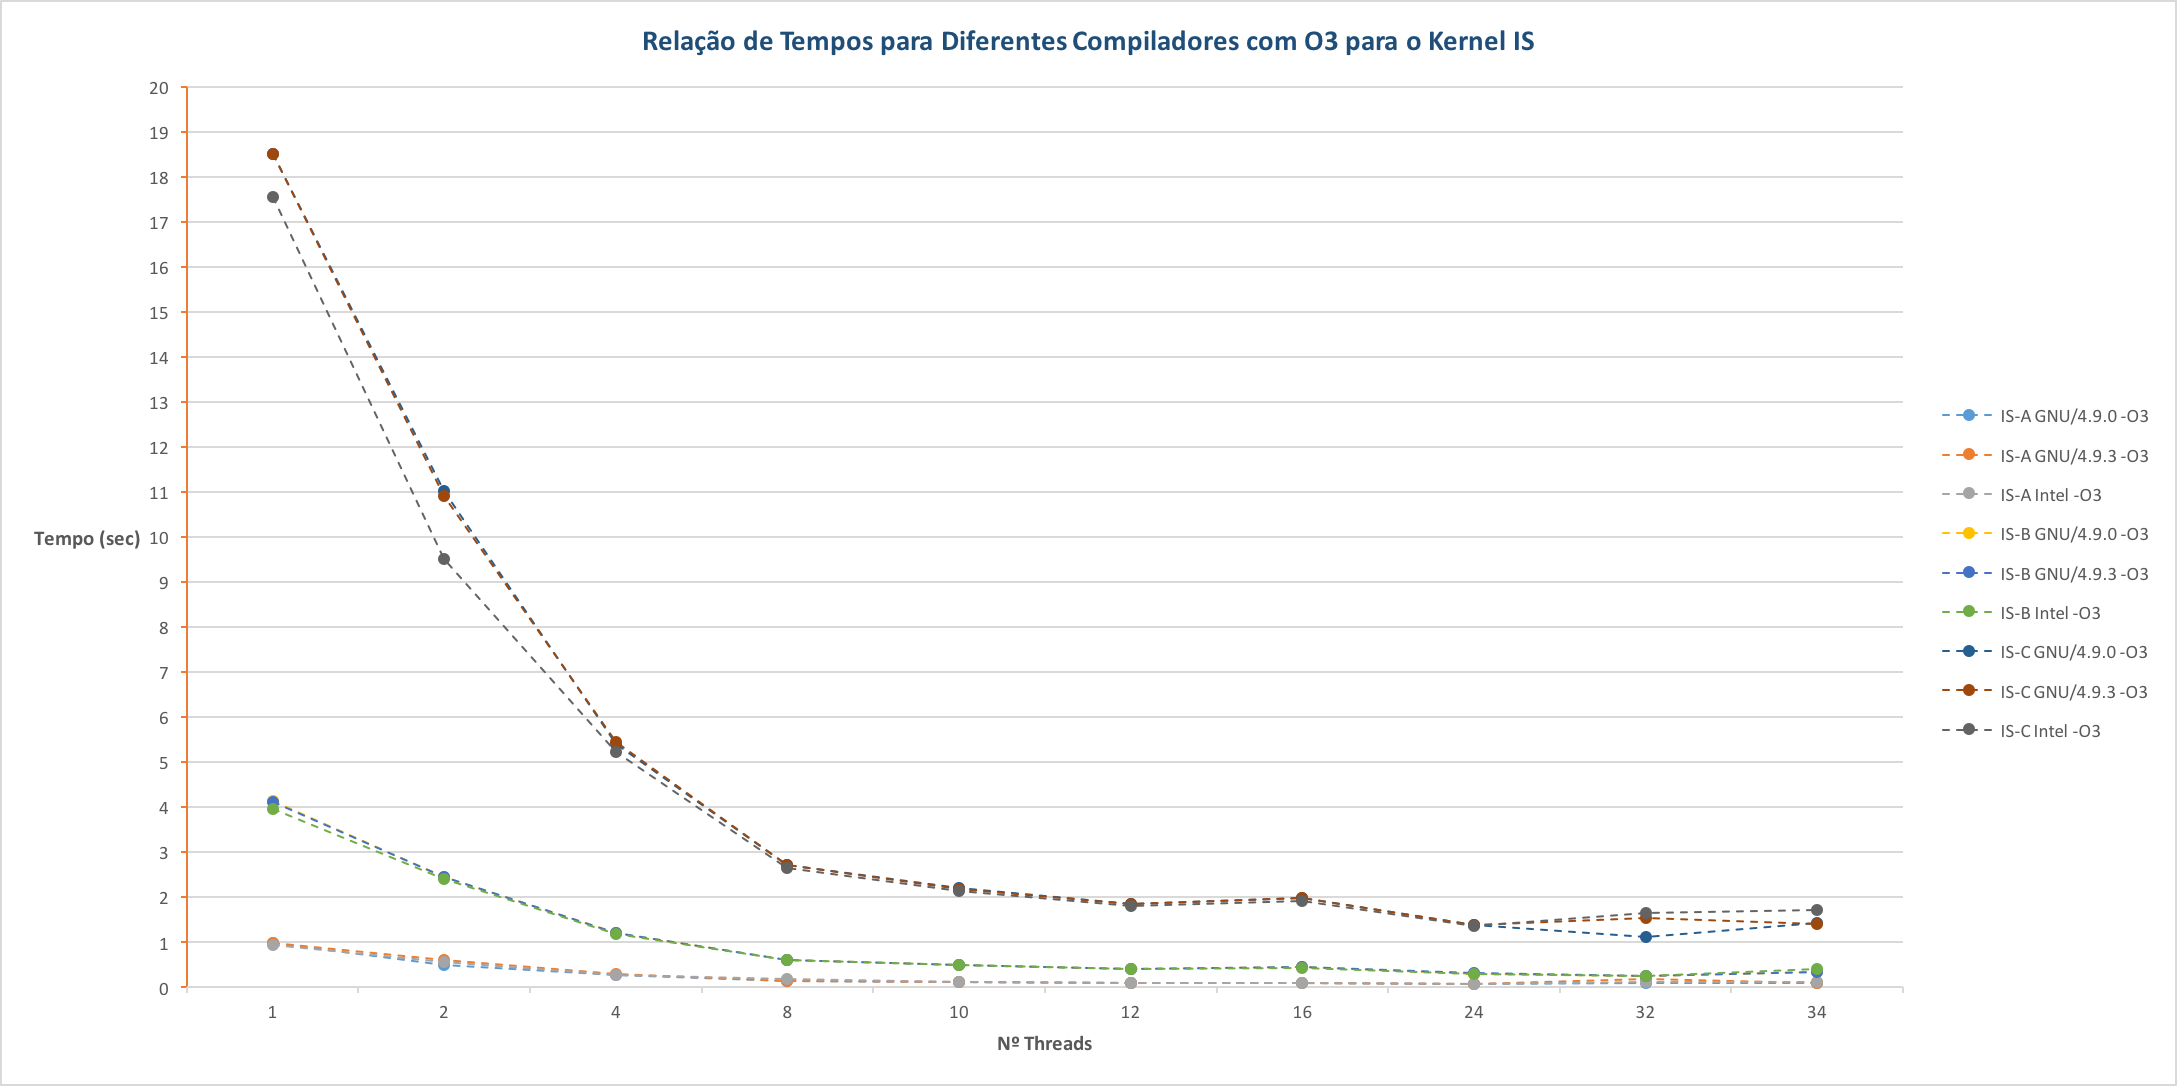
\includegraphics[scale=0.25]{OMP/tempos_dif_comp-O3_IS_nodo-641.png}
\caption{Tempos para Diferentes Compiladores com Flags -O3 para o \textit{Kernel} IS}
\end{figure}

\begin{figure}[h!]
\centering
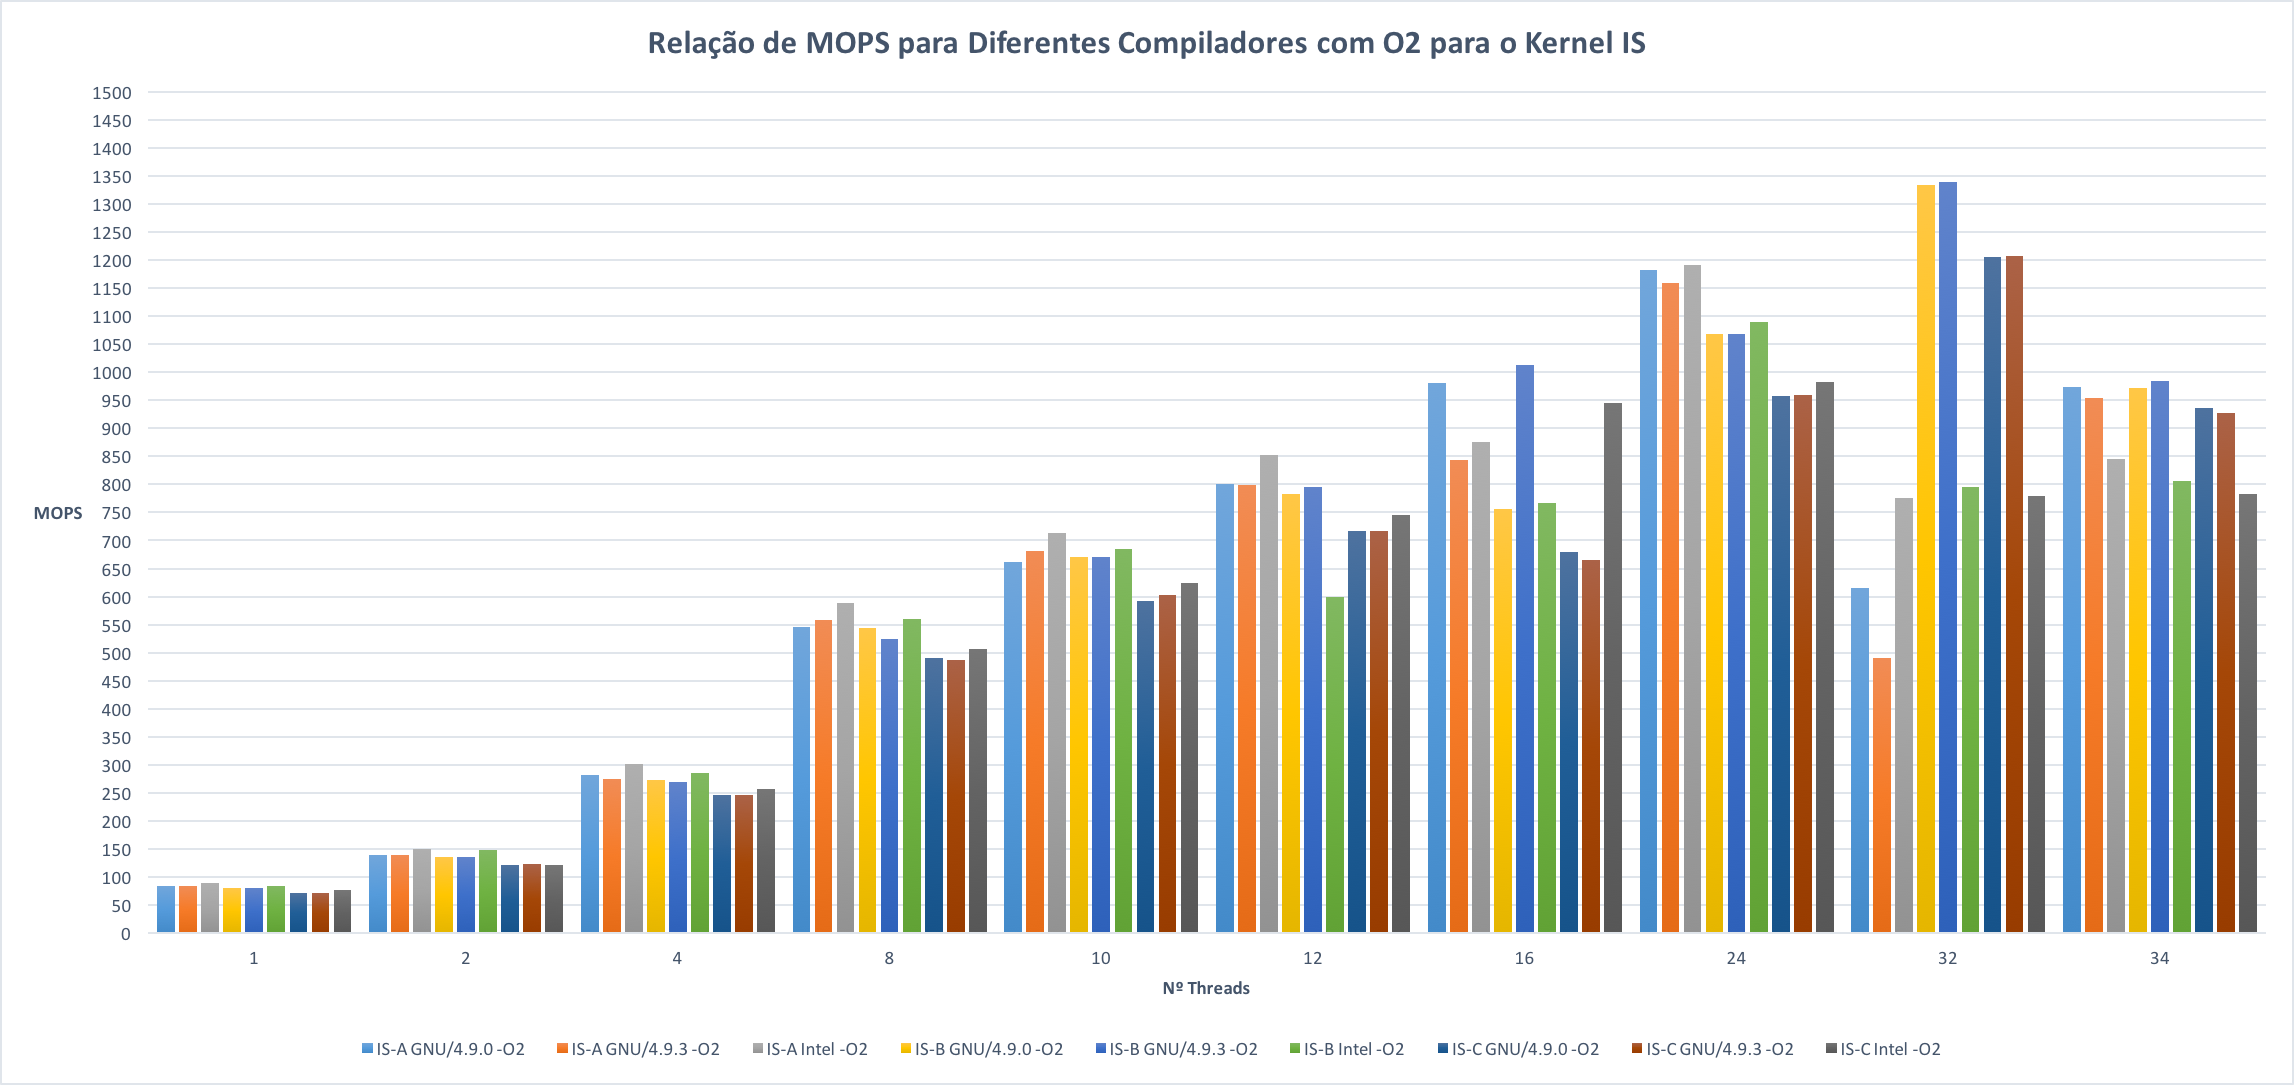
\includegraphics[scale=0.225]{OMP/mops_dif_comp-O2_IS_nodo-641.png}
\caption{MOPS para Diferentes Compiladores com Flags -O2 para o \textit{Kernel} IS}
\end{figure}

\begin{figure}[h!]
\centering
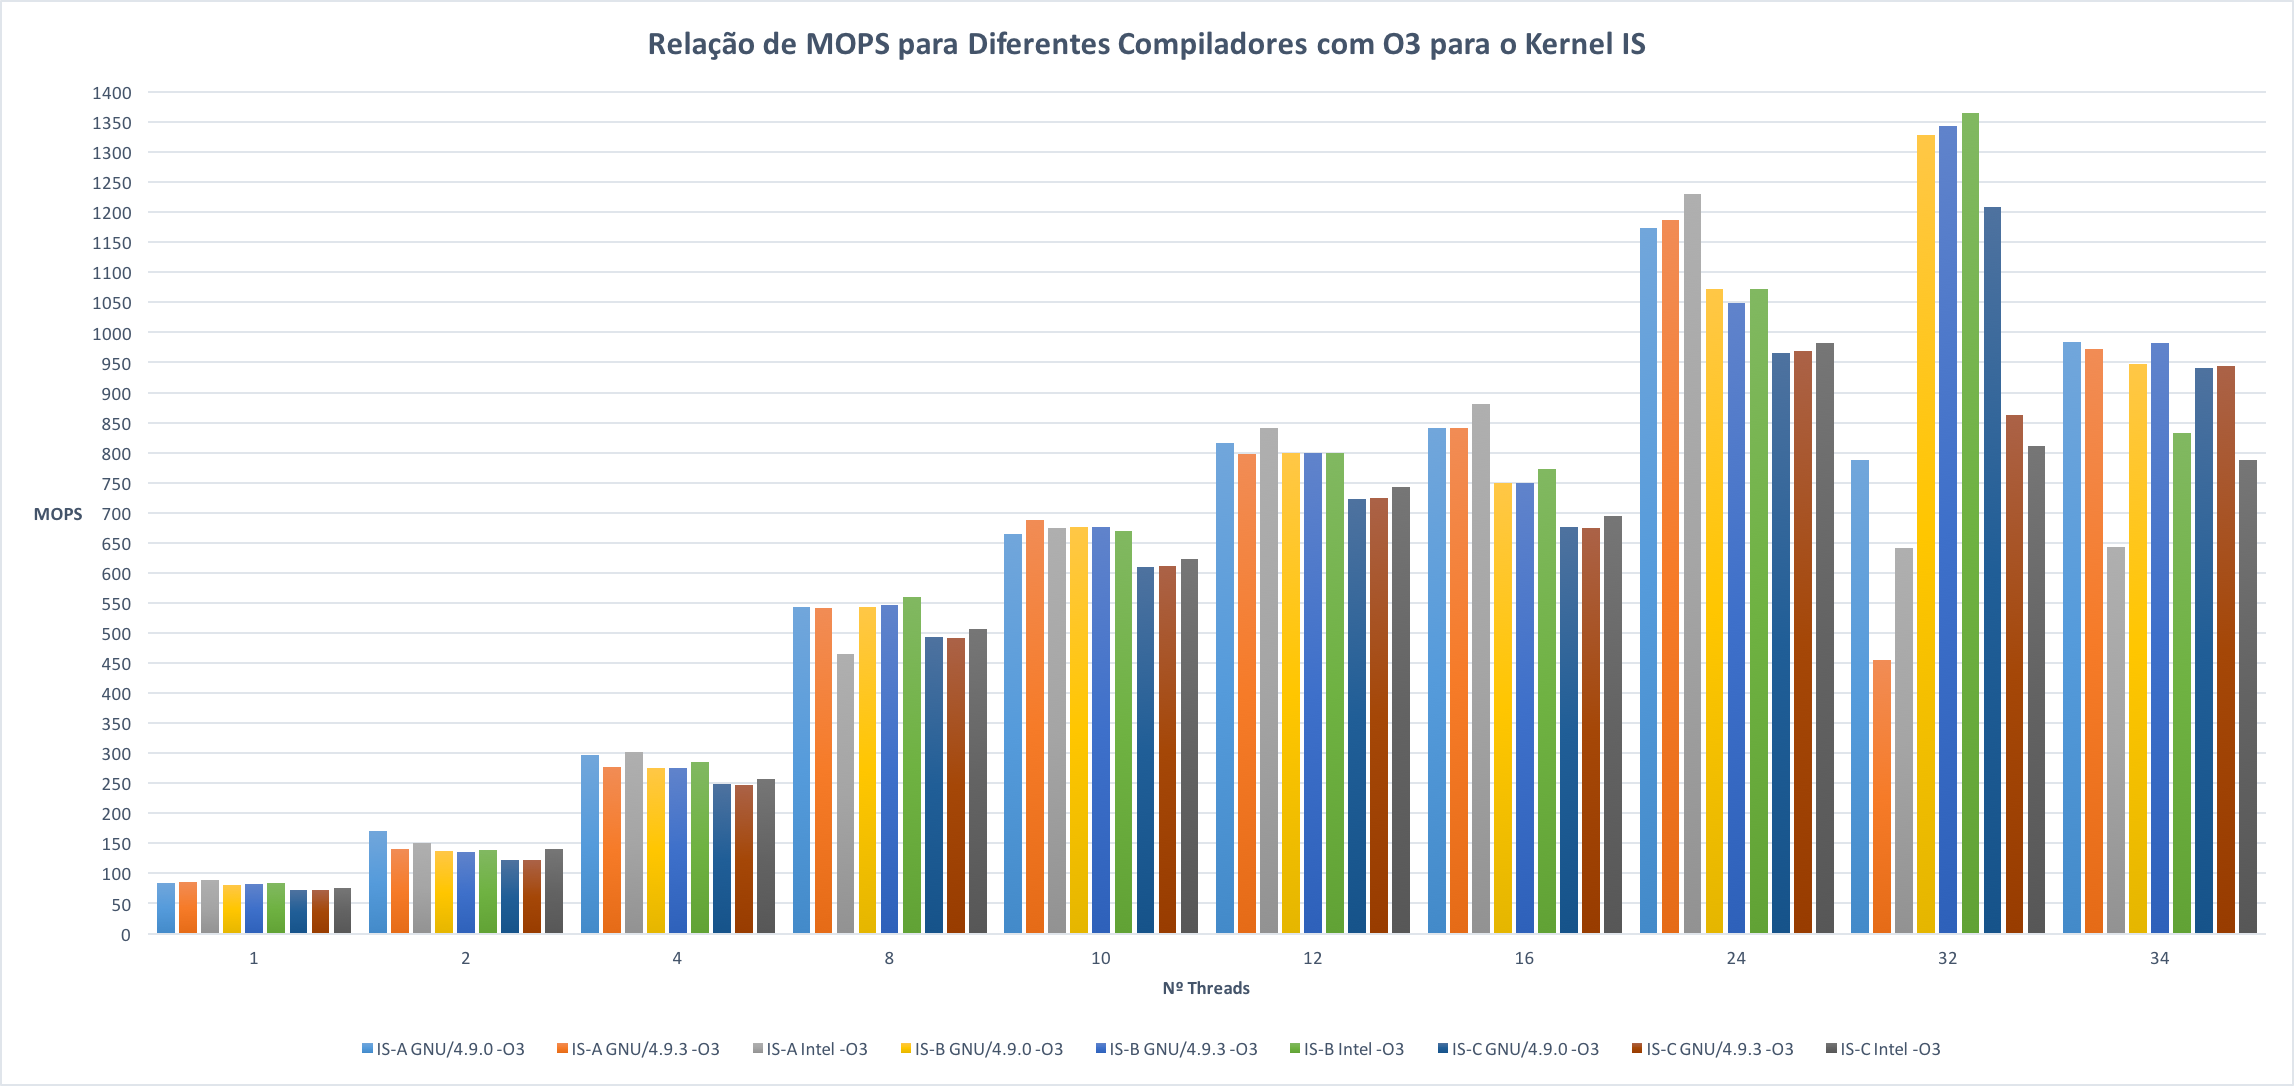
\includegraphics[scale=0.225]{OMP/mops_dif_comp-O3_IS_nodo-641.png}
\caption{MOPS para Diferentes Compiladores com Flags -O3 para o \textit{Kernel} IS}
\end{figure}

\begin{figure}[h!]
\centering
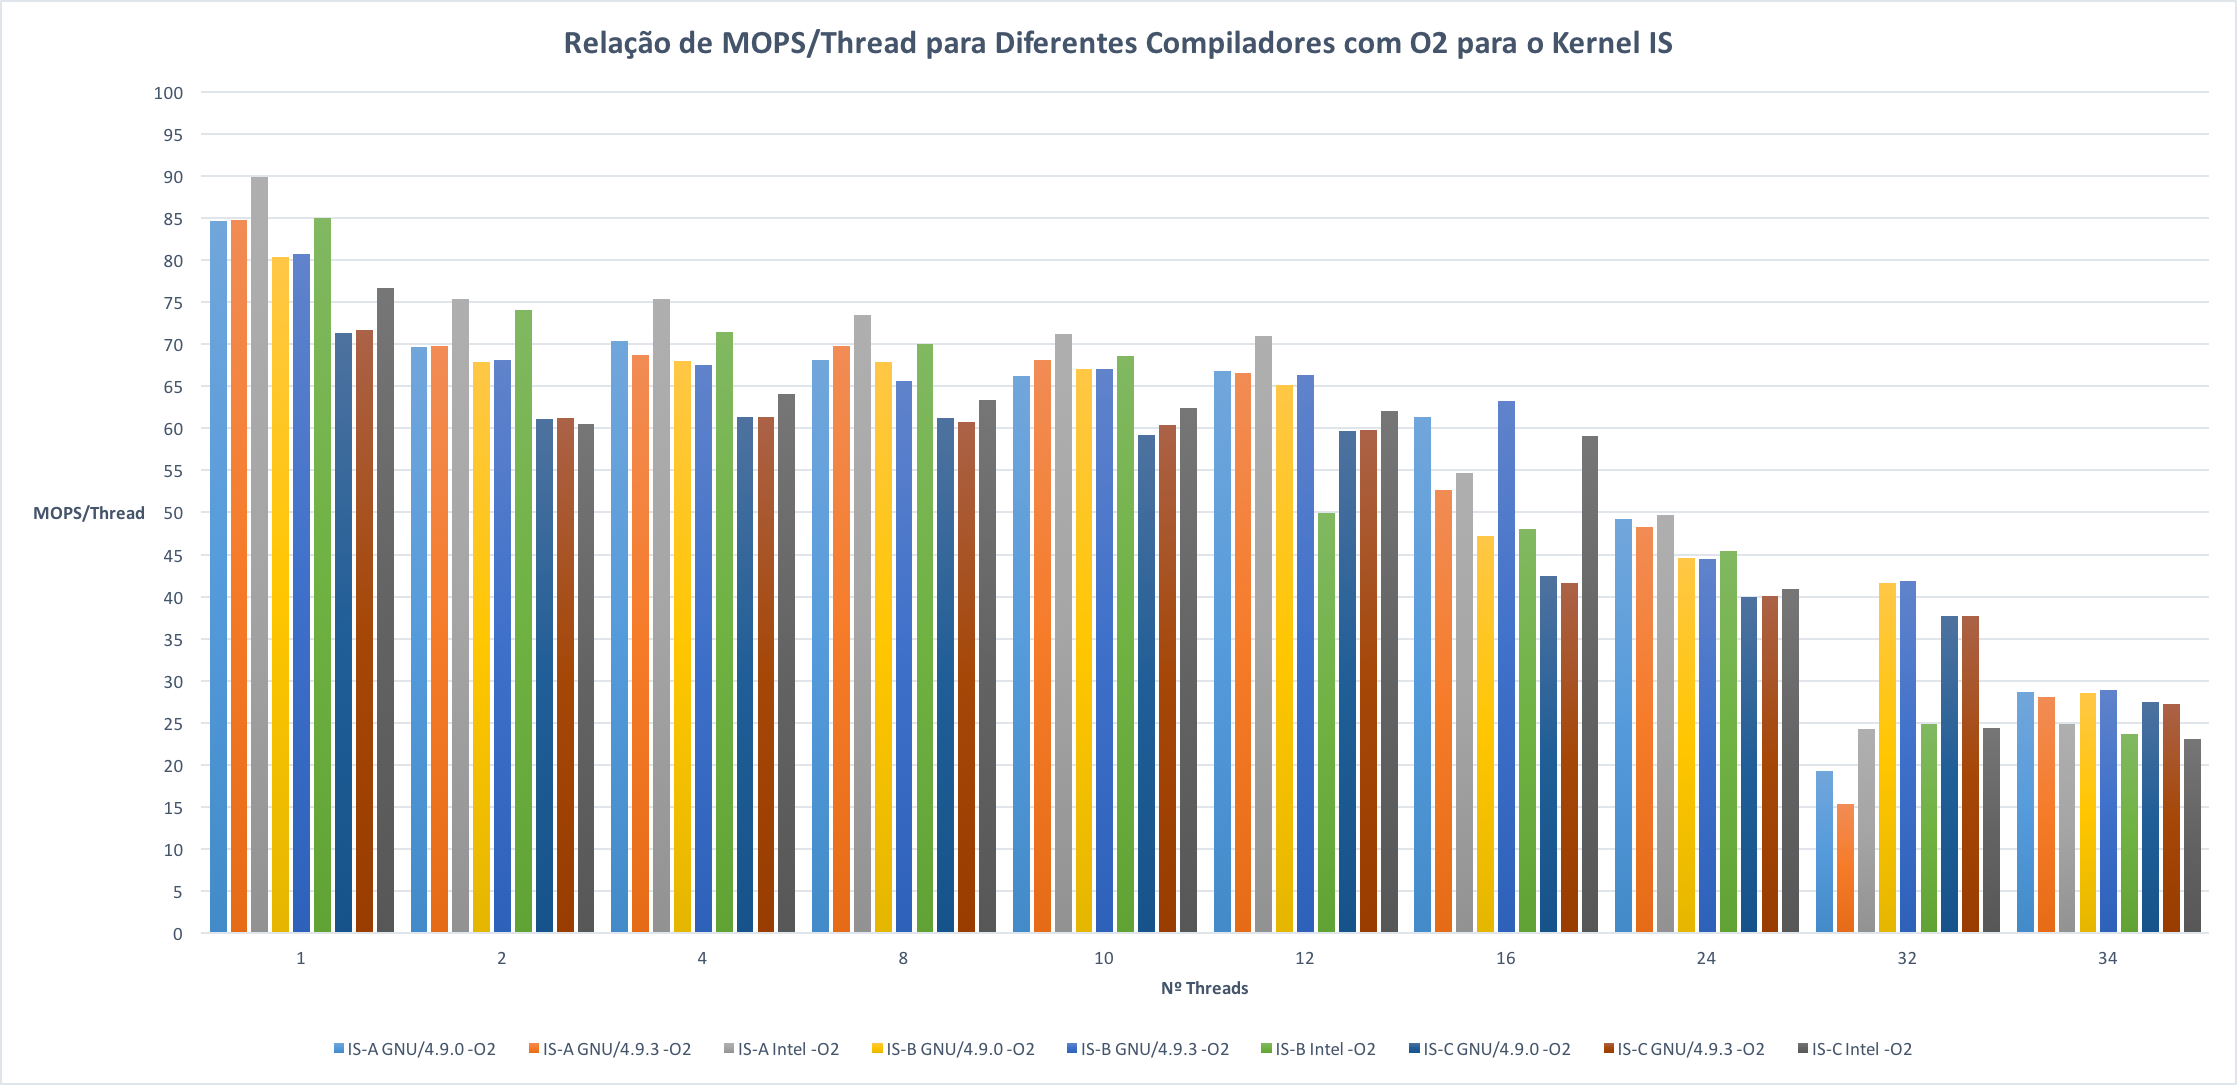
\includegraphics[scale=0.225]{OMP/mops-thread_dif_comp-O2_IS_nodo-641.png}
\caption{MOPS/\textit{Thread} para Diferentes Compiladores com Flags -O2 para o \textit{Kernel} IS}
\end{figure}

\begin{figure}[h!]
\centering
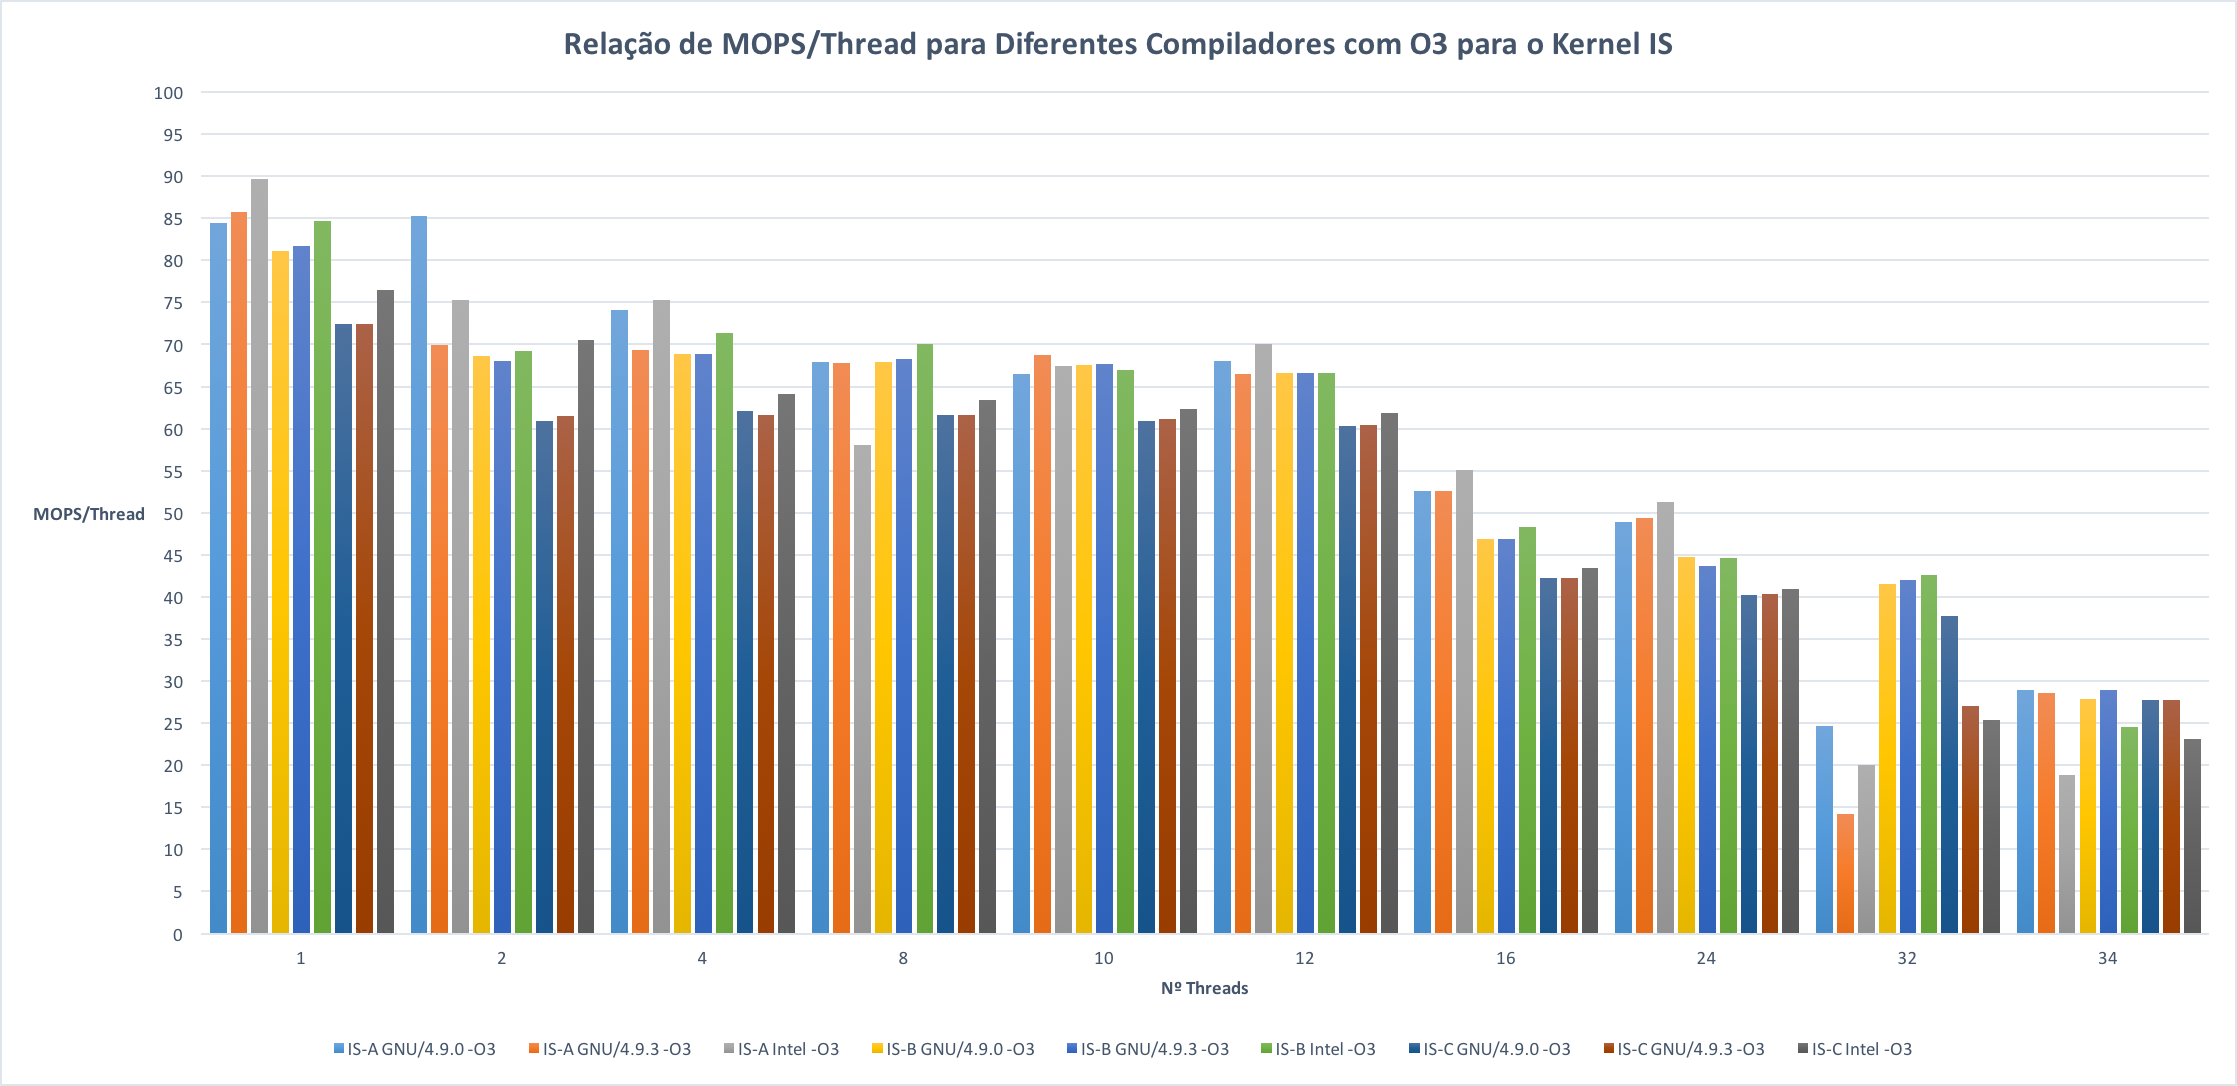
\includegraphics[scale=0.225]{OMP/mops-thread_dif_comp-O3_IS_nodo-641.png}
\caption{MOPS/\textit{Thread} para Diferentes Compiladores com Flags -O3 para o \textit{Kernel} IS}
\end{figure}

% that's all folks
\end{document}


